% Pro kompilaci po částech (viz projekt.tex), nutno odkomentovat a upravit
%\documentclass[../projekt.tex]{subfiles}

\chapter{Úvod}
Tato práce má za úkol vytvořit rychlou implementaci algoritmu nejbližšího souseda definovaného nad množinou bodů a bodem, kde samotný problém tkví v~nalezení nejbližšího bodu k~zadanému bodu z~oné množiny. Tento algoritmus lze zobecnit na hledání k-nejbližších sousedů takového bodu. Tato práce rovněž implementuje vyhledávání podobně orientovaných blízkých bodů podle nastavených kriterií.

Tyto algoritmy se využívají v~oblastech umělé inteligence, robotiky, počítačové grafiky a jiných. Podle aplikace jsou struktury optimalizovány pro různé parametry: doba stavby, rychlost získání nejbližšího souseda, paměťovou náročnost, chování v~mnohodimenzionální prostorech a jiné. Základní struktury využívají pouze dělení prostoru na různě definované pod-části ať už binární, nebo jiné, které poté řadí do stromových struktur a značně zvyšují efektivitu vyhledávání. Jiné struktury využívají různých technik pro seskupení blízkých bodů a tím sníží rozsah prohledávaných oblastí, ale za to mohou snížit přesnost. 

Prezentovaná struktura je náročná na výstavbu, ale principiálně nabízí nalezení nejbližšího souseda v~téměř konstantním čase. Této vlastnosti je docíleno promyšleným použitím hašovací tabulky, binárního vyhledávání, Voronoi diagramu a vyhledávacího oktalového stromu. Jednotlivé vrstvy jsou uspořádány do pyramidové struktury, kde se jedna vrstva vystavuje na základě té předešlé, čímž vznikne struktura optimalizována primárně na rychlost vyhledávání. Tato varianta využívá, jak prostorové struktury, tak dokonce~i techniku seskupování.

Cílem práce bylo najít a naimplementovat strukturu umožnující nejrychlejší možné vyhledávání nejbližších (orientovaných) sousedů. V~kritických místech, kde to bylo možné a efektivní byly navrhnuty formy optimalizací pomocí vektorizace a paralelizace ať už pro stavbu nebo vyhledávání. Implementace byla podrobena testům, jenž odhalily její silné ale i slabé stránky a poskytly kontext v~nichž je vhodné takovouto strukturu použít a jaké se dají očekávat výsledky. 

V~kapitole \uv{Akcelerační, prostorové a optimalizační struktury a algoritmy nad nimi} je rozebrán teoretický úvod většiny komplexnějších konceptů použitých při implementaci. Na tento úvod navazuje kapitola věnující se tomu, jakým způsobem byly jednotlivé teoretické koncepty zkombinovány do jedné struktury a jsou zde uvedeny koncepce toho, jak funguje vyhledávání a výstavba struktury. V~této kapitoly je zmíněno jakým způsobem bude implementace testována, jak po výkonnostním, tak po správnostní stránce. Následující kapitola popisuje, jak byli koncepty z~předešlé kapitoly přetvořeny na program. Popisuje jaké knihovny a jak byly použity a zmiňuje zajímavosti z~implementační části této práce. 

\chapter{Akcelerační, prostorové a optimalizační struktury a algoritmy nad nimi}
\label{teorie}

Efektivní implementace algoritmu nejbližšího souseda mohou pro zrychlení používat různé prostorové, ale i jiné struktury.  Při optimalizacích implementace těchto struktur je možné použít speciální instrukce, které vektorizují nebo jinak zrychlují klíčové části implementace. V~této sekci je možné nalézt příklady několika struktur, které se dají použít pro implementaci nejen algoritmu nejbližšího souseda, ale mohou se používat i jinde. Mimo to je níže možné najít i popis procesu vektorizace a použití vektorových optimalizací. 

\section{Hašovací tabulka}

Hašovací tabulka, někdy je možné setkat se i s~názvem slovník nebo mapa, je datová struktura umožnující přístup k~datům pomocí klíče neboli vstupní hodnoty. Této vlastnosti je dosaženo pomocí dobře zvolené funkce, které se říká hašovací. Vlastnosti funkce jsou rozebrány v~sekci níže. O~vkládání a vyhledávání v~této struktuře je možné se dočíst níže v~sekcích o~vkládání a kolizích.

\begin{figure}[!b]
    \centering
    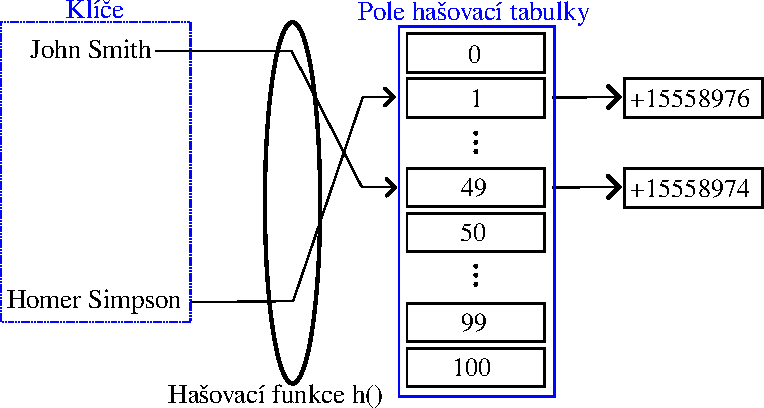
\includegraphics[width=0.5\textwidth]{obrazky-figures/hash/HT_desc.pdf}
    \caption{
Na obrázku lze vidět strukturu hašovací tabulky s~příkladem vložení jmen \uv{John Smith} a \uv{Homer Simpson} do tabulky. Hašovací funkce $h()$ se používá k~určení pozice v~tabulce, přiřazuje jména do různých indexů v~poli. \uv{John Smith} odkazuje na index 49, zatímco \uv{Homer Simpson} na index 1. Jména jsou použita jako klíče pro přístup k~telefonním číslům.
}
    \label{fig:hash_definition}
\end{figure}


\subsection*{Hašovací funkce}
Hašovací funkce je definována jako $h(k): K \rightarrow Y $, kde $K$ je množina vstupních prvků, zpravidla struktur a $Y$ je interval, na který $h$ zobrazuje. Vlastnosti funkce $h$ jsou dále rozebrány v~sekci věnující o~vlastnostem hašovací funkce. Tato funkce má na vstupu libovolný prvek $k$ ze vstupní množiny $K$, obvykle se hovoří o~klíčích. Tuto vstupní množinu mapuje na interval $Y$ od nuly do $M-1$, kde je $M > 0$. V~praxi se kvůli minimalizaci počtu kolizí je možné se spíše setkat s~$M > |K|$. Výstupu hašovací funkce se říká haš, nebo také otisk.\\ $M$ je velikost pole, které používá hašovací tabulka. Na obrázku \ref{fig:hash_definition} je znázorněno, jak hašovací tabulka funguje \cite{knn}.

Někdy se hašovací funkce rozděluje na dvě -- interní a externí \cite{hashtablebench}. Externí funkci je možné mezi jednotlivými konstrukcemi hašovacích tabulek měnit a slouží pro výpočet samotného haše na obecně libovolném intervalu. Tento interval je potřeba transformovat na $\left< 0,M-1 \right>$, kde M je velikost pole\footnote{Předpokládá se, že pole bude indexované od nuly.}, které je k~dispozici k~použití pro hašovací tabulku. Jedná se tedy o~vnitřní záležitost hašovací tabulky a pro hašovací funkci to není podstatné. 
V~textu dále nebude rozlišováno mezi interní a externí hašovací funkcí, bude na ně nahlíženo jako na jeden celek.

Je důležité, aby hašovací funkci bylo možné spustit nad libovolnými vstupními daty. Pokud vstupem hašovací funkce bude řetězec, hašovací funkce musí zohlednit všechny znaky v~tomto řetězci. Obdobně je tomu i u~jiných vstupů.

\subsection*{Vlastnosti hašovací funkce}
\label{char_hash_function}

Pro správnou a efektivní činnost je klíčové, aby hašovací funkce splňovala jisté charakteristiky:
\begin{enumerate}
    \item Deterministická\,--\,pro každý jeden vstup vždy vrátí stejný výstup.
    \item Dodržení rovnoměrného rozdělení po celém intervalu\,--\,hašovací funkce nebude vracet jeden otisk neúměrně častěji než otisky jiné.
    \item Rychlý výpočet\,--\,celý výkon hašovací tabulky stojí na rychlosti hašování.
\end{enumerate}
První charakteristika je nutná z~důvodu toho, aby při vyhledávání byla nalezena vždy stejná hodnota. Funkce musí pracovat jen na základě jediného vstupu\,--\,klíče. Zachování rovnoměrného rozdělení je nutné především, nejen však v~případech, když je interval na který hašovací funkce zobrazuje menší než mohutnost vstupní množiny. Tím pádem musí několik klíčů vyprodukovat stejný otisk, nastane tedy kolize. O~problémech, které mohou nastat, je víc napsáno v~sekci o~kolizích. Třetí charakteristika není nutná pro samotnou funkcionalitu, ale především pro reálnou použitelnost a nasazení hašovací tabulky. Někdy se dokonce používá i strojově akcelerované hašování \cite{HWhash}.

Pokud je hašovací tabulka statická, tedy jednou se vytvoří a poté se už pouze používá k~vyhledávání, může být funkce injektivní. Poté není nutné při vkládání ani při vyhledávání řešit kolize. Vyhledávání tak bude o~to rychlejší. Pokud je kladen nárok na šetření paměti, je vhodné připravit hašovací funkci tak, aby interval, na který zobrazuje, byl stejně velký jako mohutnost vstupní množiny. V~tomto případě je ale nutné vědět, která data konkretně nebo vstupní klíče budou na vstupu hašovací funkce. Dalším omezením může být také stále náročnější nalézání ideální funkce s~rostoucí vstupní množinou \cite{KnuthDonaldErvin1998Taoc}. 

Z~otisku zpravidla není možné sestavit původní klíč. Pro účely hašovací tabulky ovšem není důležité, aby mezi klíčem a otiskem neexistoval vztah. Existuje také řada dalších vlastností, které mohou být kladeny na hašovací funkce, ale pro účely hašovací tabulky není potřeba jejich dodržení.

\subsection*{Vkládání prvků}

Před tím, než začne vkládání, je nutné mít připravené pole o~velikost $M$\,--\,tedy o~maximální velikosti intervalu.
Data v~hašovací tabulce jsou ukládána do tohoto pole. Při vkládání jsou vstupní data vložena jako vstup hašovací funkce. Výstupem je otisk, nebo-li index, na který budou data uložena. Problém může nastat v~případě, že se ve vstupní množině nachází takové dva klíče, které mají stejný otisk. Tato problematika je dále rozebrána v~části věnující se kolizím.

Při vyhledávání se hledaný klíč zahašuje. Podle určeného indexu se přejde na místo v~poli a ověří se, zda byla nalezena pro správný klíč odpovídající data.


\begin{figure}[t!]
    \centering
    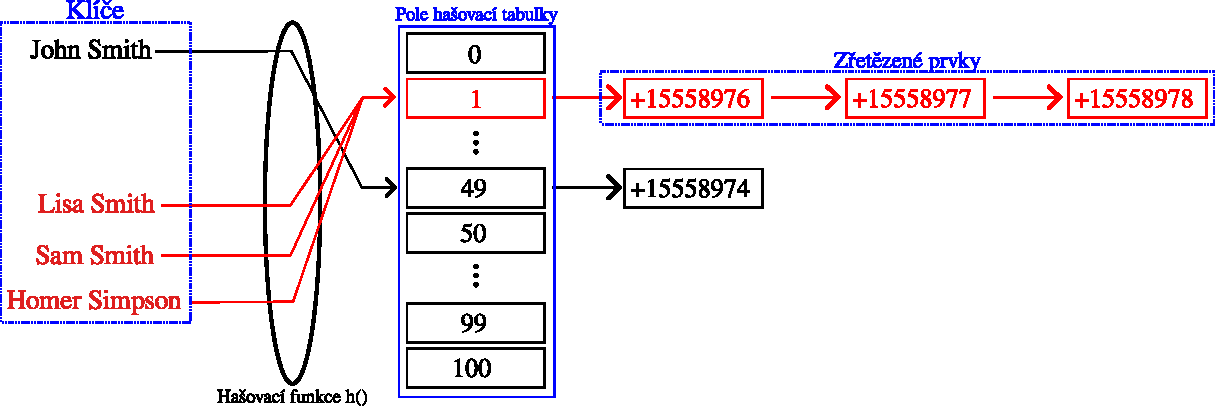
\includegraphics[width=0.9\textwidth]{obrazky-figures/hash/HT_colision.pdf}
    \caption{Hašovací tabulka používající strategii řetězení pro řešení kolizí. Hašovací funkce vygenerovala pro \uv{Homer Simpson}, \uv{Sam Smith}, \uv{Lisa Smith}, stejný otisk, znázorněno červenou. Při pokusu o~vyhledání posledního čísla bude nutné projít celou posloupnost čísel.
    }
    \label{fig:degradation_ht}
\end{figure}


\subsection*{Kolize při vkládání prvků}
\label{kolize}
Kolize v~hašovací tabulce je pojmenování pro situaci, kdy hašovací funkce pro dva různé klíče vrátí stejné otisky, tedy $h(k_1) = h(k_2)$,  $ k_1 \neq k_2$. Tato situace může nastat z~několika příčin. Může se jednat například o~nevhodně zvolenou hašovací funkci nebo příliš malý zobrazovaný interval hašovací funkce. Kolize lze řešit dvěma základními způsoby:
\begin{enumerate}
    \item Řetězením

    V~případě, že dojde ke kolizi, je prvek umístěn na stejné místo, jako již existující zařazený prvek. V~praxi se na indexech hašovací tabulky nachází struktury, které umožňují skladování více prvků. Jeden z~příkladů je použití lineárního seznamu.
    \item Otevřená adresace
    
    V~případě, kdy dojde ke kolizi, je použit alternativní způsob umístění prvku do pole. To umožňuje například použití druhé hašovací funkce, dvojitého hašování anebo připočtení k~otisku konstanty a jiné.
\end{enumerate}
Tyto strategie nejsou jediné možnosti, jakými se lze vypořádat s~kolizemi. Přinejmenším je možné tyto způsoby kombinovat. Existují však i jiné pokročilejší strategie, jak se vypořádat s~kolizemi \cite{hashtablebench}.

Kolize mohou mít velmi negativní vliv na výkonnost hašovací tabulky. Jako nejhorší případ je možné si představit situaci znázorněnou na obrázku \ref{fig:degradation_ht}. Jde o~situaci, kdy hašovací funkce bude pro mnoho prvků vracet stejný otisk. Z~toho důvodu hašovací tabulka zdegraduje ze složitosti $O(1)$ až na složitost $O(n)$, kde $n$ je počet prvků ve struktuře. Za předpokladu, že by všechny vložené prvky byly umístěny na stejný index v~poli. V~nejhorším případě je tedy při vyhledávání potřeba projít celou strukturu uchovávající prvky se stejným otiskem. 

 
\section{Detekce kolizí konvexních mnohostěnů}
Nechť existují dva konvexní mnohostěny \(K_1\) a \(K_2\). Mnohostěny \(K\) jsou zadány vrcholy \(k_0\) až \(k_n\), kde \(n \in \mathbb{N}\). 

\subsection*{Aproximace detekce kolize osově zarovnané krychle a konvexního mnohostěnu}
Nechť \(K_1\) je konvexní mnohostěn a $K_2$ je pravidelná krychle zarovnaná se souřadným systémem. Krychli lze vyjádřit prostřednictvím dvou bodů \(U_l\) a \(U_r\), určujících protilehlé vrcholy.. Potom stačí, aby alespoň jeden z~bodů mnohostěnu \(K_1\) ležel v~krychli \(K_2\), což ověřit je velmi snadné. Potom musí alespoň částečně existovat společná pod-část \(K_1\) a \(K_2\), což se dá velmi snad ověřit.

Při provedení popsaného postupu lze dojít k~nesprávnému výsledku. Taková situace je zobrazena na obrázku \ref{fig:gjk-basic}. V~některých aplikacích však tento rozdíl lze zanedbat. V~případě, že $K_1$ i $K_2$ jsou osově zarovnané krychle, tak není možné, aby tato detekce někdy fungovala špatně \cite{3D_colision_survey}.


\begin{figure}
     \begin{subfigure}[t]{0.45\textwidth}
    
    \centering
    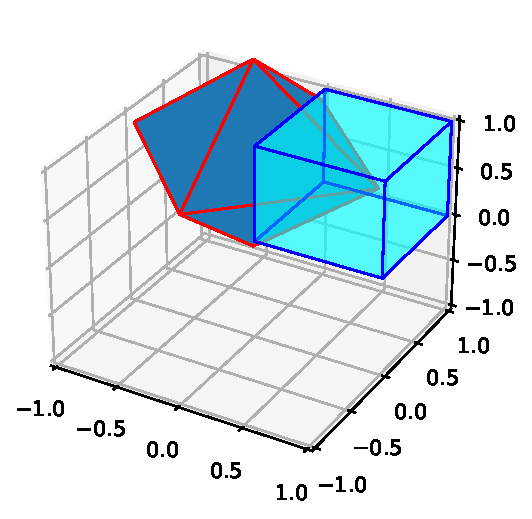
\includegraphics[scale=0.7]{obrazky-figures/gjk/gjk-good.pdf}
    \caption{$K_1$ a $K_2$ zobrazeny v~prostoru. Jeden z~vrcholů $K_2$ je uvnitř krychle $K_1$.
    }
\end{subfigure}
    \hfill
     \begin{subfigure}[t]{0.45\textwidth}
    
    \centering
    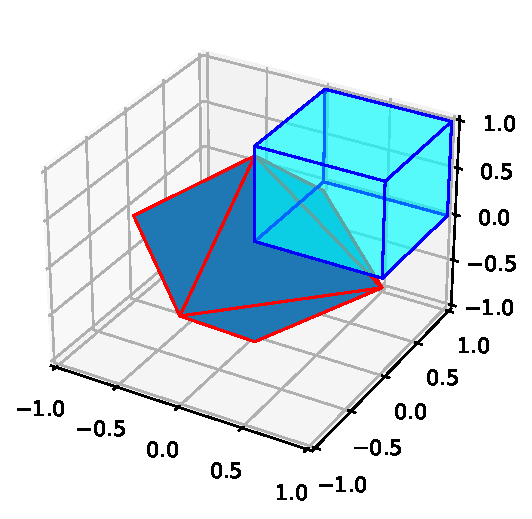
\includegraphics[scale=0.7]{obrazky-figures/gjk/gjk-notgood.pdf}
    \caption{$K_1$ a $K_2$ zobrazeny v~prostoru. Žádný z~vrcholů $K_2$ není uvnitř krychle $K_1$ a přesto mají společnou podčást.}
\end{subfigure}

   \caption{Porovnání dvou situací při průniku krychle a konvexního mnohostěnu.} 
    \label{fig:gjk-basic}

    
\end{figure}

\subsection*{Minkowského rozdíl}
V~angličtině je znám pod pojmem \emph{Minkowski difference} \cite{minikowski}, je množina bodů obecně v~\(p\)-dimenzionálním prostoru, která vyjadřuje vztah mezi dvěma objekty \(A\) a \(B\). Tyto objekty jsou zadány vrcholy. Její výpočet probíhá iterativně, kdy je nutné projít všechny kombinace vrcholů a nad každou dvojicí je vypočten jejich rozdíl, čímž vznikne nová množina \(C\) o~mohutnosti \(M = |A| \cdot |B|\), což zkomplikuje konstrukci pro objekty s~mnoha vrcholy. Množina \(C\) obsahuje vektory, tak, jak jsou znázorněny na obrázku \ref{fig:minikowski-dif}.

Vzniklé body je možné uzavřít do konvexní obálky \cite{minikowski}, čímž vznikne tvar, jak je možné vidět na obrázku \ref{fig:minikowski-c}, jehož poloha reprezentuje vzájemnou pozici, tedy zdali jsou v~kolizi nebo ne. Pokud se v~této obálce nachází i počátek souřadného systému, znamená to, že jsou ony objekty v~kolizi. Diskutovanou situaci a zobrazení výpočtu je možné vidět na obrázku \ref{fig:minikowski-kolizion}. Formálně zapsaný vztah lze vyjádřit\footnote{\url{https://www.youtube.com/watch?v=MDusDn8oTSE&}} \cite{minikowski}:

\[
A-B=\{ \mathbf {a} -\mathbf {b} \,|\,\mathbf {a} \in A,\ \mathbf {b} \in B\}
\]


\begin{figure}
     \begin{subfigure}[t]{0.45\textwidth}
    
    \centering
    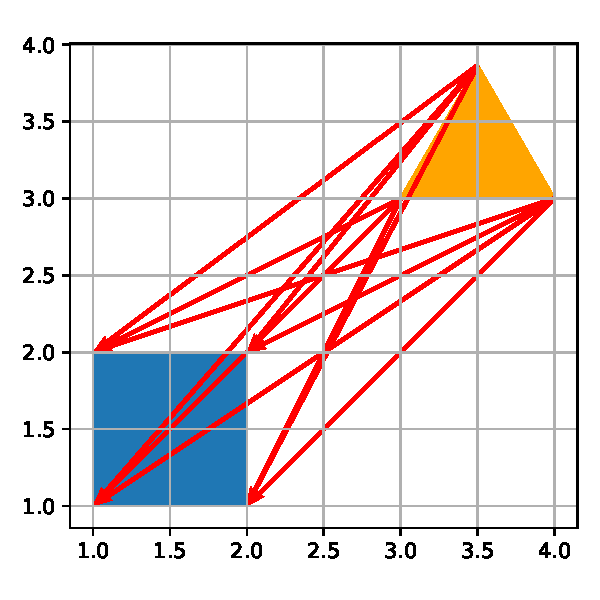
\includegraphics[scale=0.7]{obrazky-figures/gjk/minkowksi_desc.pdf}
    \caption{Grafické znázornění výpočtu množiny Minkowského rozdílů.
    }
    \label{fig:minikowski-dif}
    
\end{subfigure}
    \hfill
\begin{subfigure}[t]{0.45\textwidth}
    
    \centering
    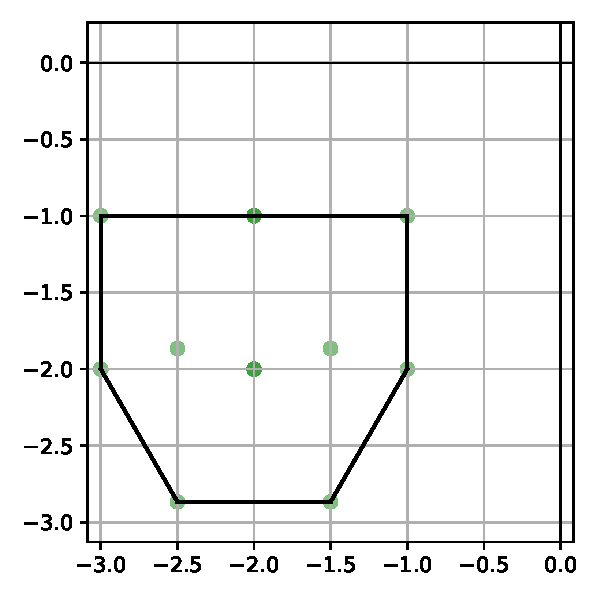
\includegraphics[scale=0.7]{obrazky-figures/gjk/minkowksi_c.pdf}
    \caption{Body z~Minkowského rozdílů jsou vykresleny zelenou barvou. Body jsou obklopeny nejmenší konvexní obálkou pro tyto body.}
    \label{fig:minikowski-c}
    
\end{subfigure}

\caption{Minkowského rozdíl.}
    \label{fig:minikowski}

    
\end{figure}


\begin{figure}


\begin{subfigure}[t]{0.29\textwidth}
    
    \centering
    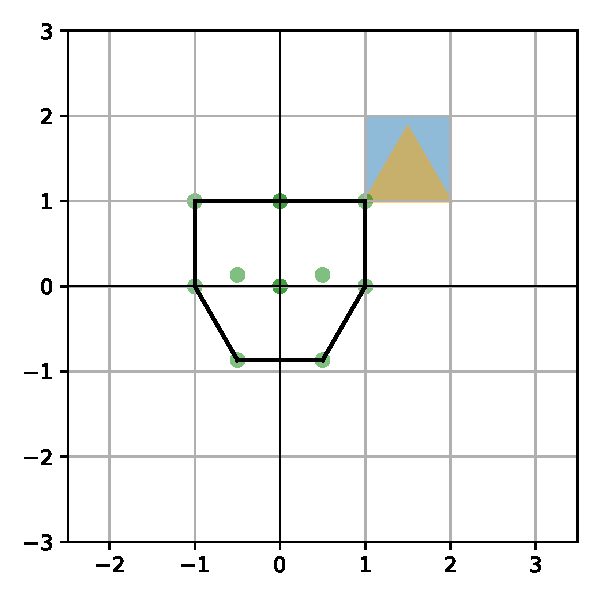
\includegraphics[scale=0.5]{obrazky-figures/gjk/minkowksi_overlap.pdf}

\end{subfigure}
\hfill
\begin{subfigure}[t]{0.29\textwidth}
    
    \centering
    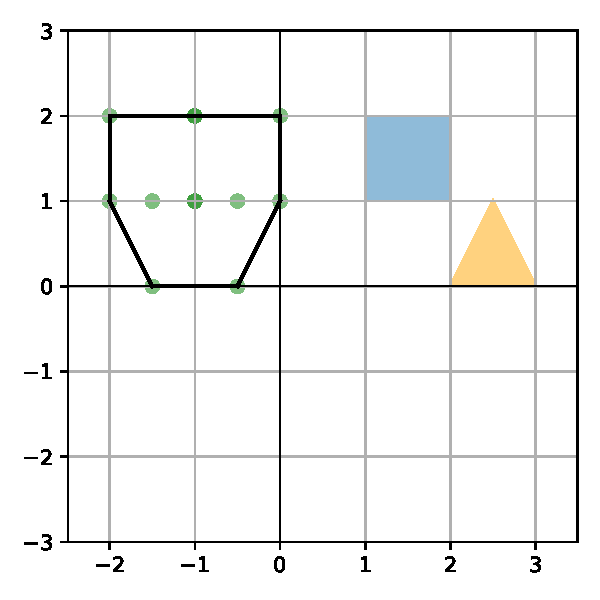
\includegraphics[scale=0.5]{obrazky-figures/gjk/minkowksi_notoverlap.pdf}

    
\end{subfigure}
\hfill
\begin{subfigure}[t]{0.29\textwidth}
    
    \centering
    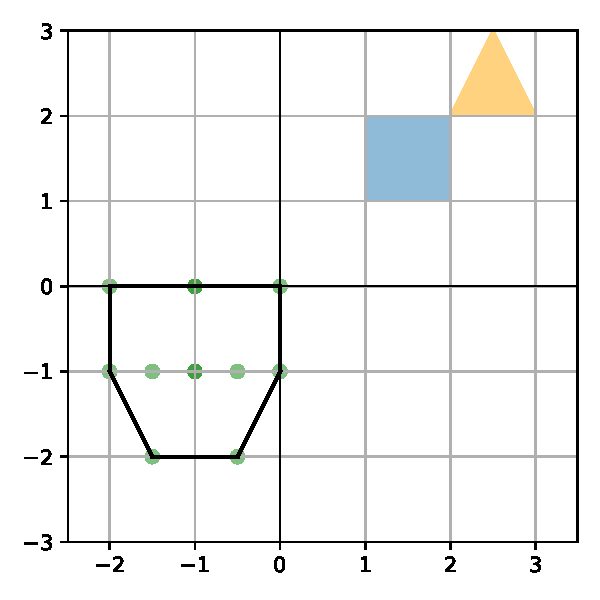
\includegraphics[scale=0.5]{obrazky-figures/gjk/minkowksi_notoverlap2.pdf}
    
\end{subfigure}

   \caption{Z~obrázku lze vyčíst, jakým způsobem se chová množina daná Minkowského rozdílem v~různých pozicích, především pak při kolizi (vlevo).
   } 
    \label{fig:minikowski-kolizion}

\end{figure}

\subsection*{Algoritmus GJK}
Algoritmus Gilbert--Johnson--Keerthi (GJK) \cite{initialGJK} využívá vlastnosti získatelných z~Minkowského rozdílu, ale vzhledem k~tomu, jak roste výpočetní náročnost s~množstvím dimenzí a vrcholů, je obvykle velmi náročné vypočítat tuto množinu. Je třeba tedy minimalizovat počet výpočtů, který je potřebný k~detekci kolize.

Obecný GJK algoritmus má na výstupu vzdálenost dvou objektu. Existují i varianty, které jsou optimalizované jen pro odpověď ano/ne.

\subsubsection{Support funkce}

Při pohledu na obrázek \ref{fig:minikowski-kolizion} lze vidět, že pro určení, zda jsou dva objekty v~kolizi, stačí použít pouze okrajové body -- tedy ty, které tvoří onu konvexní obálku a dokonce i snad nejsou potřeba všechny body, ale jen některé v~blízkosti počátku souřadného systému. Tyto body lze poznat pomocí toho, že jsou nejvzdálenější od středu ve směru \(D \in \mathbb{R}^p\):

\[
\max(D \cdot (A~- B)),
\]
což nikterak nepomůže při optimalizaci složitosti, ta je stále \(O(|A| \cdot |B|) = O(n^2)\). Nicméně při roznásobení a použití funkce \(\max\) pro oba členy samostatně vznikne vztah\footnote{\url{https://winter.dev/articles/gjk-algorithm}}:

\[
\max(D \cdot A) - \max(-D \cdot B)\footnote{Pro zachování funkčnosti je potřeba pro B obrátit směr D.} ,
\]
který lze řešit v~lineárním čase \(O(|A| + |B|) = O(n)\). Popsaný postup se nazývá v~angličtině \emph{Support function} a vypočítává z~Minkowského rozdílů pouze to nejnutnější. Výsledkem je jediný vrchol Minkowského rozdílů, jak lze vidět na obrázku \ref{fig:supportfunction}. Pak už je otázkou několika iterací pro získání dostatečně velké části obálky, aby bylo možné rozhodnout, zda se počátek souřadného systému nachází uvnitř \cite{initialGJK}.

\begin{figure}[t]
    \centering
    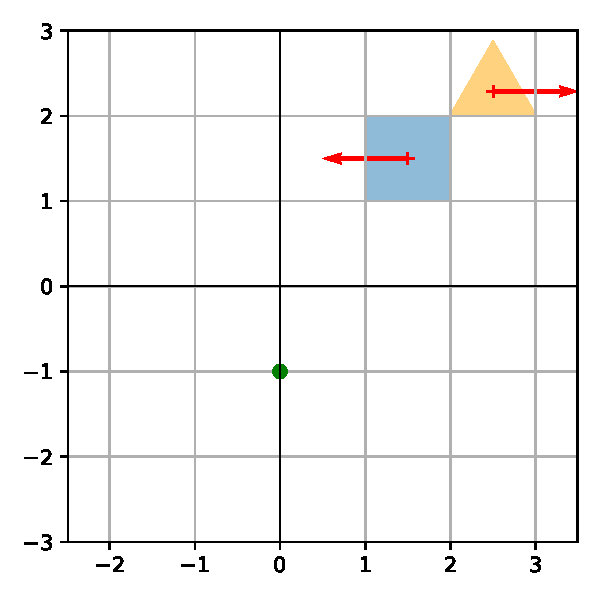
\includegraphics[scale=0.7]{obrazky-figures/gjk/support.pdf}
    \caption{Vypočítaný bod (označený zelenou barvou) pomocí funkce support pro směr (1,0) respektive (-1,0), označený červenou barvou. }
    \label{fig:supportfunction}
\end{figure}

\subsubsection{Simplex}
Nejednoduší tvar pro výběr oblasti v~obecně \(p\) dimenzionálním prostoru se nazývá simplex. Tedy pro \(p=1\) se jedná o~bod, pro \(p=2\) úsečku pro \(p=3\) trojúhelník a $p=4$ čtyř stěn. Je potřeba tedy $p+1$ bodů. Tento tvar pro účely GJK algoritmu reprezentuje nějakou pod-část vzniklé obálky z~Minkowského rozdílů. Postupnou iterací lze nalézt simplex, který je nejblíže počátku a má tedy největší šanci, že do něj bude patřit počátek souřadného systému, čímž se dosáhne tíženého výsledku a odpoví na otázku, zda jsou dva konvexní tvary v~kolizi \cite{initialGJK}.

Otázkou může být jakým způsobem bude algoritmus aktualizovat směr $D$, protože pro stejný směr by funkce support vracela stále stejný bod. Simplex bude pro $p=3$ tvořen jedním až čtyřmi body. Směr $D$ aktualizuje funkce $\mathrm {NearestSimplex} (s)$, která má na vstupu simplex $s$ a na základě něj se rozhodne, jak se vypočítá další směr. Tedy při každé iteraci algoritmu je výstupem funkce $\mathrm {NearestSimplex} (s)$ nový směr a případně odpověď, zda jsou v~kolizi. Simplex může obsahovat jeden z~těchto tvarů:

Pro přehlednost je simplex struktura s~kapacitou $p+1$ bodů, která umožňuje vkládat prvek na nulté místo a zbytek prvků posune o~jedno a případně přebytečné body zahodí. Dále pak nultý prvek bude označován jako bod $a$, první $b$ a tak dále. 

\subsubsection{Bod}
Pokud je simplex jen jeden bod $a$, tak se směr $D$ změní na směr k~počátku souřadného systému. Nový směr je znázorněn na obrázku \ref{fig:gjk_point}.

\subsubsection{Úsečka}
V~případě, že simplexem je úsečka, je dána dvěma body $a$ a $b$. Nový směr bude vypočítán jako normálový vektor ve směru k~počátku
\ref{fig:gjk_line}.

\subsubsection{Trojúhelník}
V~případě, že simplexem je trojúhelníkem, tak už dokáže vybrat oblast, ve které by potenciálně mohl být počátek souřadného systému. Celá situace je znázorněna na \ref{fig:gjk_triangle}.


\begin{figure}
\begin{subfigure}[t]{0.3\textwidth}
         \centering
    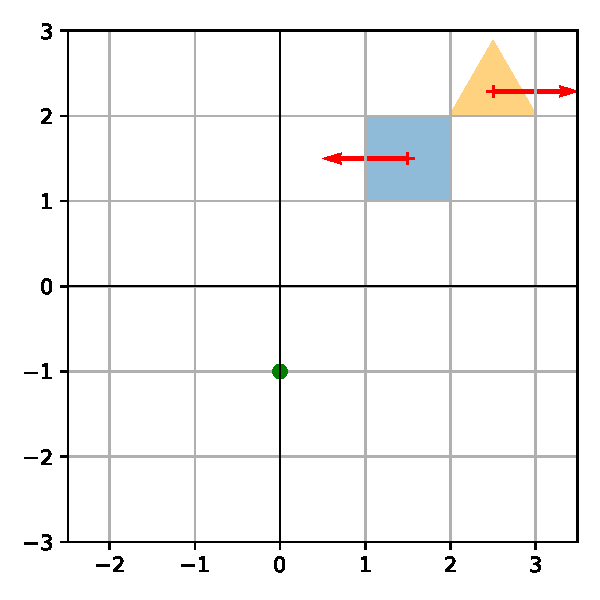
\includegraphics[scale=0.5]{obrazky-figures/gjk/gjk_point.pdf}
    \caption{Simplex sestavený z~jednoho bodu. Nový směr pro, který bude vypočítán nový bod z~Minkowského rozdílu (označený zelenou barvou).}
    \label{fig:gjk_point}
     \end{subfigure}
\hfill
\begin{subfigure}[t]{0.3\textwidth}
         \centering
    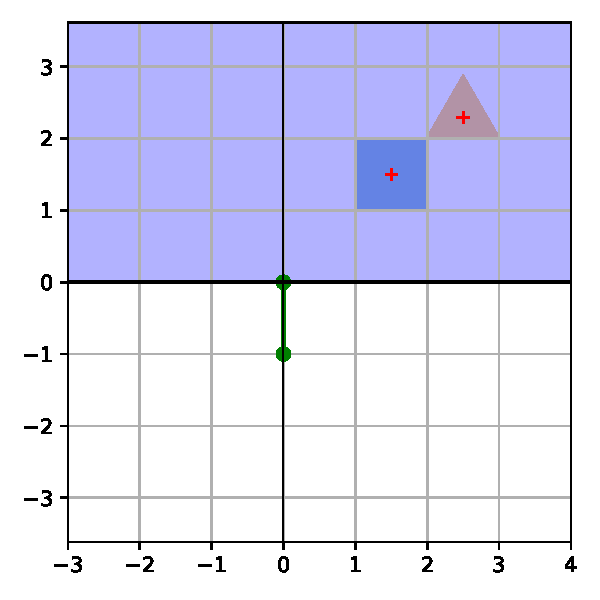
\includegraphics[scale=0.5]{obrazky-figures/gjk/gjk_line.pdf}
    \caption{Simplex sestavený ze dvou bodů (označený zelenou barvou). Je třeba provést kontrolu, zda nově vzniklý bod je v~sekci (znázorněné modrou barvou), která by umožnila vznik trojúhelníku obsahující počátek souřadného systému. Na obrázku nově vzniklý bod je v~této oblasti (nachází se na hranicích). Na obrázku není vidět směr $D$, neboť bude určen jako (0,0).}
    \label{fig:gjk_line}
\end{subfigure}
\hfill
\begin{subfigure}[t]{0.3\textwidth}
    \centering
    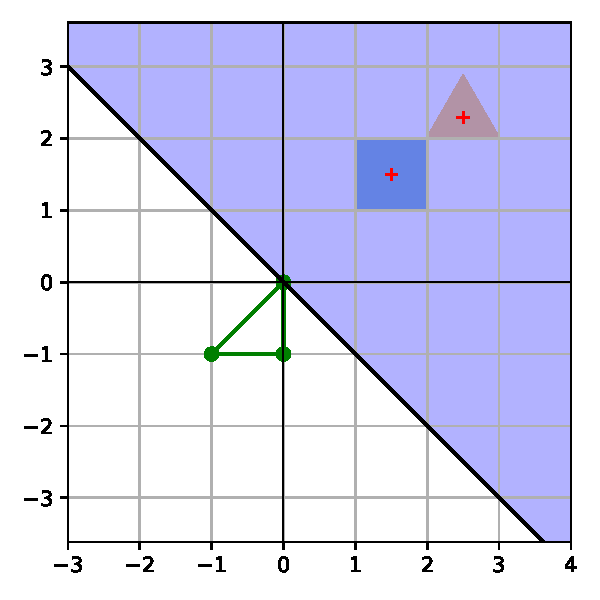
\includegraphics[scale=0.5]{obrazky-figures/gjk/gjk_triangle_bad.pdf}
    \caption{Simplex sestavený ze tří bodů\,--\,označený zelenou barvou ve tvaru trojúhelníku. Je třeba zkontrolovat, zda se nově vzniklý bod nachází v~sekci (znázorněné modrou barvou), která by umožnila vznik trojúhelníku obsahující počátek souřadného systém. Na obrázku nově vzniklý bod není v~této oblasti. Algoritmus skončí a vrátí \emph{false}.}
    \label{fig:gjk_triangle}
     \end{subfigure}

    \caption{Algoritmus GJK při ne-kolizi.}
\end{figure}


\begin{figure}
\begin{subfigure}[t]{0.45\textwidth}
         \centering
    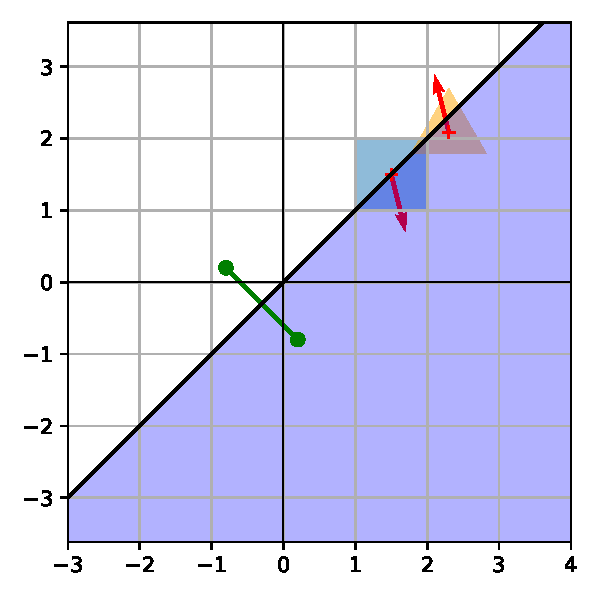
\includegraphics[scale=0.5]{obrazky-figures/gjk/gjk_line_2.pdf}
    \caption{Simplex sestavený ze dvou bodů\,--\,označený zelenou barvou. Je třeba zkontrolovat, zda se nově vzniklý bod nachází v~sekci (znázorněné modrou barvou), která by umožnila vznik trojúhelníku obsahující počátek souřadného systém. Na obrázku nově vzniklý bod je v~této oblasti.}
    \label{fig:gjk_line_cols}
    
\end{subfigure}
\hfill
\begin{subfigure}[t]{0.45\textwidth}
    \centering
    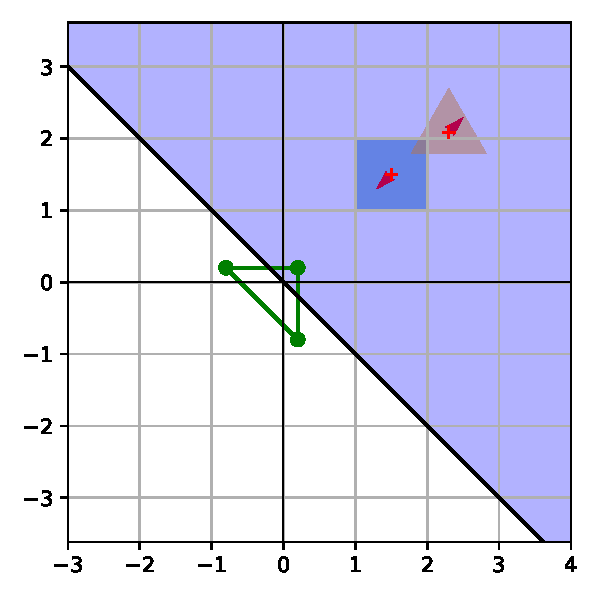
\includegraphics[scale=0.5]{obrazky-figures/gjk/gjk_triangle_2.pdf}
    \caption{Simplex sestavený ze tří bodů (označený zelenou barvou ve tvaru trojúhelníku). Je třeba zkontrolovat zda se nově vzniklý bod nachází v~sekci (znázorněné modrou barvou), která by umožnila vznik trojúhelníku obsahující počátek souřadného systém. Na obrázku nově vzniklý bod je v~této oblasti. Mimo to vzniklý trojúhelník vytvořil obal kolem počátku, algoritmus končí a vrací \emph{true}.}
    \label{fig:gjk_triangle_cols}
     \end{subfigure}
\caption{Algoritmus GJK při kolizi.}
    
\end{figure}


\subsubsection{Čtyřstěn}
Pokud je potřeba detekovat kolize pro $p=3$ prostor, tak je potřeba uvažovat o~případě, kde je simplex zadán čtyřmi body. V~takovém případě se jedná o~čtyřstěn.  


\subsection*{Hlavní cyklus algoritmu}
Nechť existuje simplex $s = \emptyset$ a je stanovena maximálně mohutnost, jako $p+1$, dále pak existuje směr $D$, zvolený například jako konstanta $(1,0)$. Poté existují dva konvexní tvary $A$ a $B$, které jsou dány vrcholy. Příklad hlavního cyklu může vypadat a:
\begin{enumerate}
    \item Vypočtení nové hodnoty $support$ z~funkce $Support$ pro tvary $A$, $B$ a směr $D$.
    \item simplex = $\{support\}$ a $direction = -support$.
    \item Opakuj:
    \begin{enumerate}
    \item $support = Support(A,B,D)$.
    \item Pokud $(dot(support, D) <= 0)$, tak nemůže dojít ke kolizi.
    \item Do simplex množiny je vložen nový prvek a v~případě, že množina dosáhla maximální velikosti, je poslední získaný bod vyloučen z~množiny.
    \item Pokud funkce $NextSimplex(s, D)$ vrátí \emph{true}, tak je $A$ a $B$ v~kolizi. Jinak opakuj.    
    \end{enumerate}
\end{enumerate}










%NNNNNNNNNNNNNNNNNNNNNNNNNNNNNNNNNNNNNNNN
\section{Problém nejbližšího souseda a Voronoi diagramy}
\label{nn}

Funkce k-nejbližšího souseda je obvykle založena na Euklidovské vzdálenosti mezi vstupním bodem a vstupní množinou bodů. Euklidovskou vzdálenost lze obecně definovat pro body mající $p$ dimenzí. Pro výpočet vzdálenosti mezi dvěma body $x_i$ a $x_j$ je možné použít následující vzorec \cite{knn}:
\label{euklid}
\[
d(x_i, x_j) = \sqrt{(x_{i1} - x_{j1})^2 + (x_{i2} - x_{j2})^2 + \cdots + (x_{ip} - x_{jp})^2}.
\]


\begin{figure}

     \begin{subfigure}[b]{0.45\textwidth}
     % \vspace{-1mm}
     
\centering
\begin{tikzpicture}
\begin{axis}[
    % MV: opravdu to ma byt takto?
    axis equal image,
    %axis lines=middle,
    xmin=-0, xmax=1, % rozsah na ose x
    ymin=0, ymax=1, % rozsah na ose y
]
\addplot [only marks, red,  mark=+] table {data/points.txt};
% MV: opraven compile error 
% <3
\addplot [mark=none, update limits=false] table {data/Voronoi.txt};
\end{axis}
\end{tikzpicture}


\end{subfigure}
     \begin{subfigure}[b]{\textwidth}
     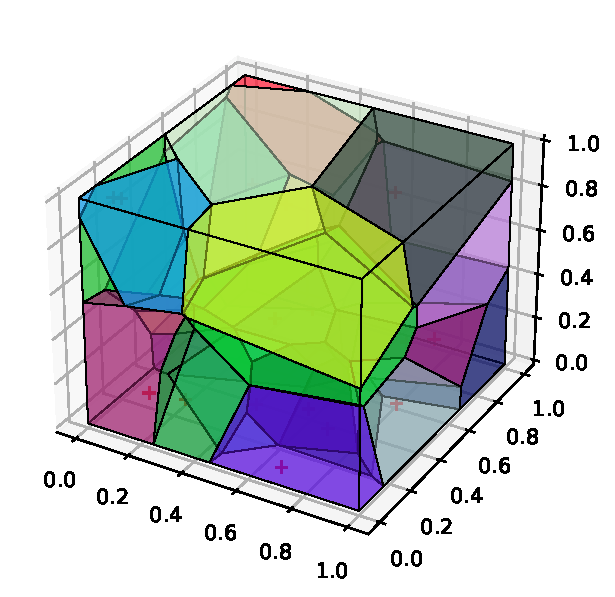
\includegraphics[scale=0.7]{obrazky-figures/nn/voronoi_3D.pdf}
     
     \end{subfigure}



\caption{Každý z~obrázků obsahuje 20 označených bodů (označených \uv{+}) a jejich Voronoi diagram, pro $p = 2$ a $p = 3$.}
\label{voro_def}

     
\end{figure}

Přirozený způsob grafického znázornění myšlenky problému nejbližšího souseda je pomocí Voronoi diagramu \cite{octreehash}. Toto lze vidět na obrázku \ref{voro_def}. V~diagramu se nachází 20 označených bodů pomocí \uv{+} a příslušné Voronoi buňky $R_i$, které obklopují každý bod. Každá Voronoi buňka $R_i$ je množinou všech bodů, pro které platí, že má: nejmenší vzdálenost k~bodu $x_i$. Tento vztah lze definovat \cite{knn}

\[
R_i = \{x \in \mathbb{R}^p : d(x, x_i) \leq d(x, x_m), \forall i \neq m\},
\]
kde $R_i$ je Voronoi buňka pro bod $x_i$. Při pohledu na obrázek \ref{voro_def} lze vidět, že ať už je vybrán jakýkoliv bod z~oblasti Voronoi buňky $R_i$, tak jeho nejbližší sousedem bude vždy bod $x_i$. Další zkoumání prozradí, že pokud je potřeba najít pro vstupní bod jeho nejbližší bod náležící do množiny vstupních bodů, bude tento bod určen nejbližší hranou Voronoi buňky. Druhou z~vlastností je patrný problém k-nejbližších sousedů. Tento problém je možné dále definovat, jako přiřazení testovanému bodu $k$ nejbližších bodů ze vstupní množiny bodů. V~praxi je obvykle hodnota $k$ zvolena jako liché číslo, aby se předešlo remízám. Obvykle pro $k = 1$ se nehovoří o~problému prvního-nejbližšího souseda ale přímo o~problému nejbližšího souseda \cite{knn}.

\section{Prostorové struktury}
Prostorové struktury jsou velmi často využívány v~mnoha oborech informatiky, jakožto například ve strojovém učení, robotice, geografických informačních systémech a také v~počítačové grafice. Častou aplikací prostorových struktur v~počítačové grafice je problém nejbližšího souseda \cite{balltree}.






\subsection*{Octree a quadtree}
\label{octree}
Oktalové stromy, octree nebo quadtree jsou relativně jednoduché prostorové datové struktury, které pracují na principu rozdělování podprostoru na poloviny v~každé dimenzi. Pokud jsou zadány body v~3D prostoru, tak se hovoří o~octree, protože když je prostor v~každé dimenzi rozdělen na polovinu, tak vznikne 8 krychlí. Pokud jsou použity pouze 2 dimenze, vzniknou 4 čtverce\,--\,tedy quadtree. Vzhledem k~nevýhodám, o~kterých se hovoří níže, se tato struktura obvykle používá především pro nižší počet dimenzí \cite{octreehash}.

\begin{figure}[b!]
     \centering
     \begin{subfigure}[b]{0.45\textwidth}
         \centering
         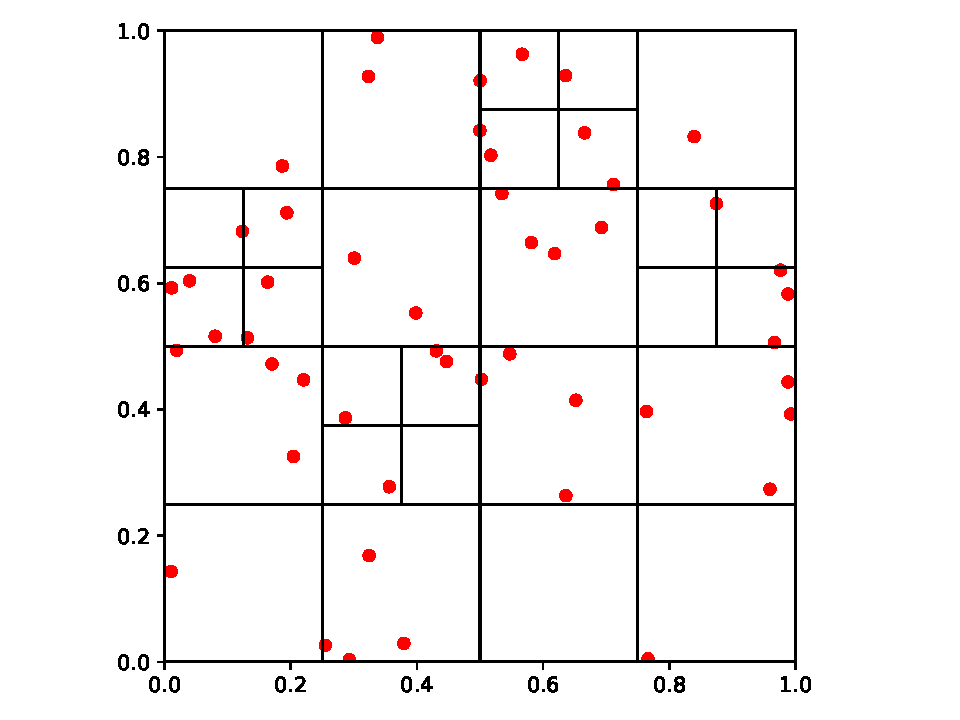
\includegraphics[width=\textwidth]{obrazky-figures/octree/octree-good.pdf}
         \caption{Rovnoměrně náhodně rozložených 50 bodů. Maximální hloubka stromu je 3, pro $m = 3$.}
         \label{subfigure:50randompoints}
     \end{subfigure}
     \hfill
     \begin{subfigure}[b]{0.45\textwidth}
         \centering
         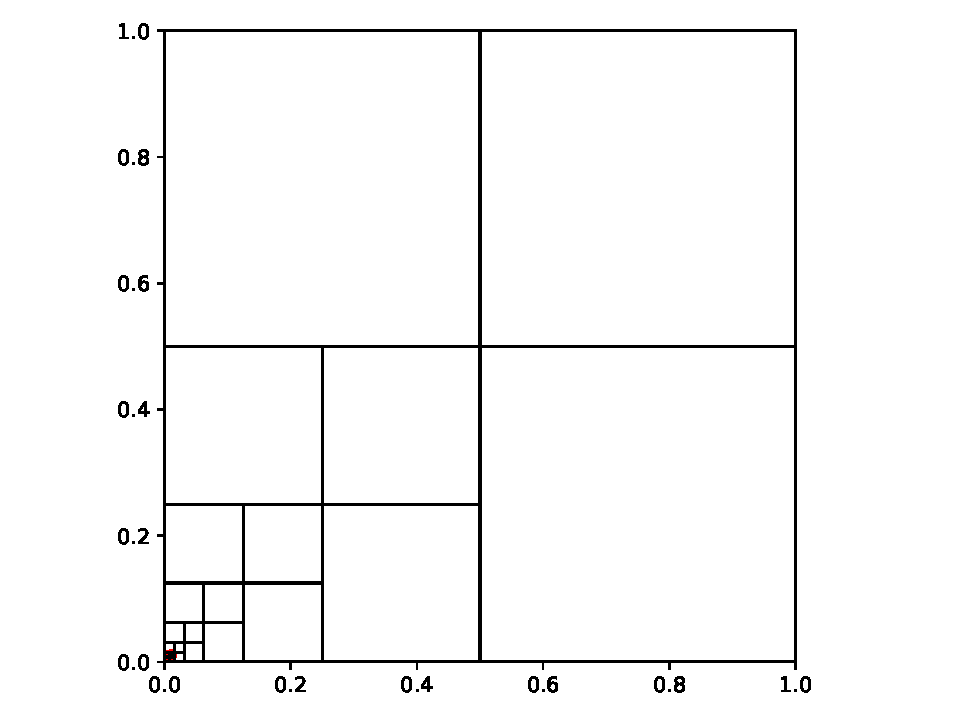
\includegraphics[width=\textwidth]{obrazky-figures/octree/octree-bad.pdf}
         \caption{Nerovnoměrně rozležení bodů, v~okolí počátku souřadného systému. Maximální hloubka stromu je 10, pro $m = 3$}
     \end{subfigure}

        \begin{subfigure}[b]{0.8\textwidth}
                     \centering
         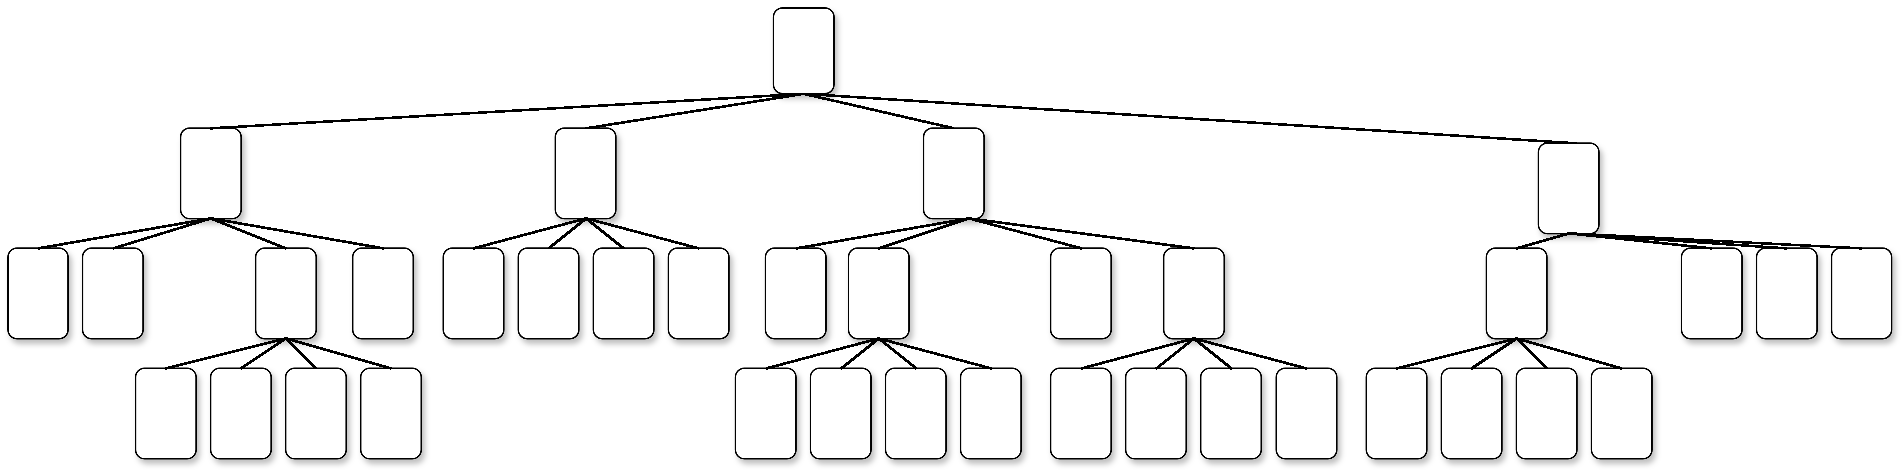
\includegraphics[width=\textwidth]{obrazky-figures/octree/octree-good_diagram.drawio.pdf}
         \caption{Stromové zobrazení quadtree pro stejné body, jako na obrázku \ref{subfigure:50randompoints}. }
        \end{subfigure}

        \caption{Porovnání hloubky quadtree pro stejné množství bodů s~jiným rozmístěním v~prostoru. }


        \label{fig:octree_bad_points}
        
        
\end{figure}


\subsubsection{Konstrukce Octree}
Prostor je tak dlouho rekurzivně dělen v~každé rovině na polovinu, dokud není splněna podmínka zastavení, zpravidla mohutnost množiny bodů v~uzlu. Rekurzivní sestupem vznikne stromová struktura, kdy každý prvek může mít $0$ až \(2^p\) synů \cite{octreehash}. 

\subsubsection{Vyhledávání nejbližšího souseda}
Algoritmus postupně, rekurzivně vylučuje uzly stromu. Začne v~uzlu listovém, do kterého by náležel bod ke kterému je hledán nejbližší soused a pak postupuje ostatními uzly dokud není vyloučeno, aby se nacházel nejbližší soused jinde \cite{kdimensiontree}:
\begin{enumerate}
    \item Algoritmus na každé úrovni rozhodne, do kterého oktetu (čtvrtiny) by připadl vyhledávaný bod, dokud nedojde až do listového uzlu $S_{leaf}$.
    \item V~listovém uzlu nalezne nejbližší bod $b$ se vzdáleností $d$.
    \item Vznikne hyperkoule\footnote{Pro $p=2$ se jedná o~kružnici, pro $p=3$ se jedná o~kouli. } $k$ s~průměrem $d$ a středem $b$. 
    \item Pokud tato kružnice $k$:
    \begin{enumerate}
        \item zasahuje i mimo listový uzel, tak je vyhledávání znovu spuštěno nad otcem $S_{leaf}$ a pokračuje se bodem 2.
        \item zasahuje pouze do oblasti dané $S_ {leaf}$, takže bod $b$ je nejbližším sousedem hledaného bodu.
    \end{enumerate}
\end{enumerate}
 

\subsubsection{Výhody a nevýhody}
Velkou výhodou octree je, že jeho implementace je velmi jednoduchá. Například knižní implementace na webu geeksforgeek\footnote{\url{https://www.geeksforgeeks.org/octree-insertion-and-searching/}} má méně než 300 řádků.

Nevýhodou ale může být i například to, že tyto datové struktury mohu vytvářet velmi hluboké stromy i pro velmi malé datové sady a jestliže se v~sadě nachází velké množství bodů u~sebe. Při dělení prostoru může hloubka stromu značně narůst a strom bude velmi řídký. Na obrázku \ref{fig:octree_bad_points} lze vidět takovou situaci. Pak strom defakto zdegraduje na lineární seznam, ve kterém je značně náročnější vyhledávání než u~stromových algoritmů. 

Další nevýhodou je to, že množství synů roste exponenciálně s~počtem dimenzí $p$. Počet synů je roven $2^p$, což u~mnoho dimenzionálních prostor může značně ovlivnit nejen dobu stavby stromu, ale i vyhledávání.
Mimo zmíněné je octree zatížen prokletím dimensionality.


%\subsubsection{Prokletí dimnezionalizy}
% Prokletí dimenzionality (angl. The course of dimensionality) je pojem, který souhrnně označuje několik různých problému, nevýhod, objevující se nejen u prostorových struktur.  







\subsection*{KD-tree}
KD-tree je binární stromová struktura, která pracuje na principu postupného dělení jedné dimenze tak, aby množinu bodů vždy rozdělila na půl \cite{moore1991kdtrees}. Tímto způsobem vznikne struktura, která se daleko lépe přizpůsobuje nepravidelnosti vstupní množiny bodů \cite{kdimensiontree}.

\subsubsection{Konstrukce KD-tree}
Vstupem pro algoritmus konstrukce KD-tree je množina bodů $S \subseteq \mathbb{R}^p$ a konstantu $M_{max}$, která určuje kolik bodů maximálně se má nacházet v~listovém uzlu \cite{moore1991kdtrees}. Na obrázku \ref{fig:kd-tree} lze vidět vystavěný KD-tree. 

KD-tree je velmi často využíván a existuje mnoho způsobů, jak může být sestaven. Zde je například uveden jednoduchý způsob, jak může být tato struktura vytvořena \cite{moore1991kdtrees}:

\begin{figure}[b!]
\begin{subfigure}[b]{1\textwidth}
    
    \centering
    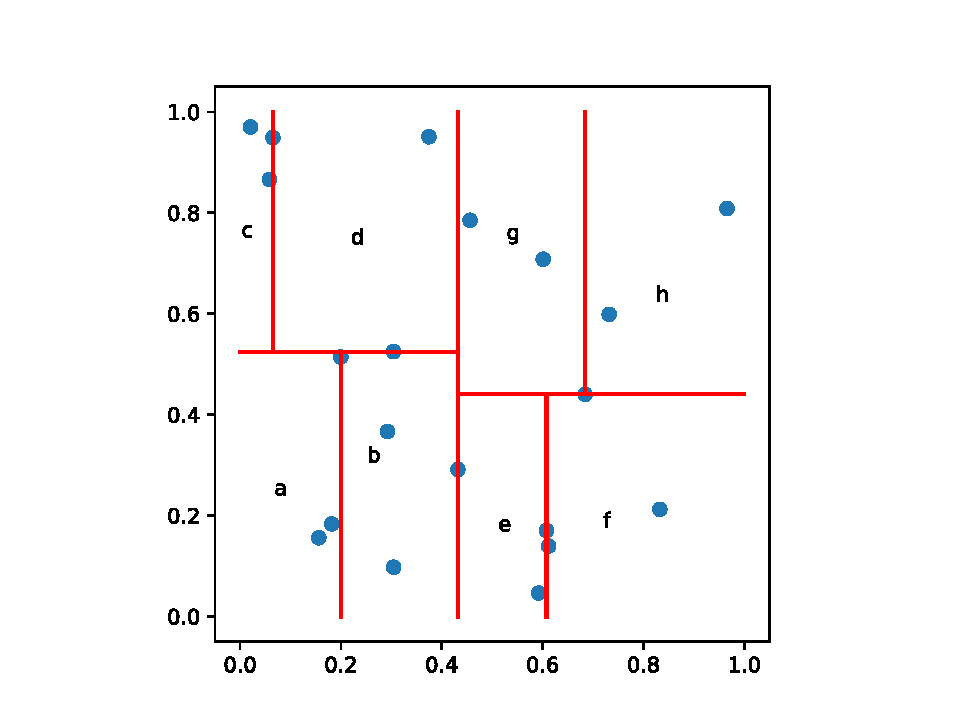
\includegraphics[scale=.6]{obrazky-figures/kdtree/kdtree.pdf}
    \caption{Vybudovaný KD-tree pro 20 bodů v~rovině.}

\end{subfigure}

\begin{subfigure}[b]{0.9\textwidth}
    
    \centering
    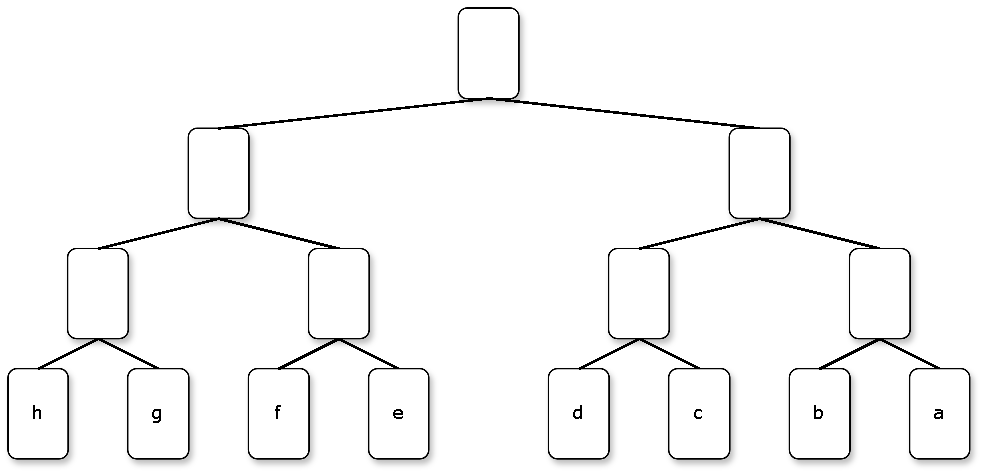
\includegraphics[scale=0.6]{obrazky-figures/kdtree/kd-tree.drawio.pdf}
\end{subfigure}
    \caption{Vybudovaný KD-tree pohled na stromovou strukturu.}

    \label{fig:kd-tree}

Existuje mnoho variant, jak vystavět KD-tree. Jedna ze základních možností je popsána v~následujících bodech:
\end{figure}
\begin{enumerate}
    \item Je vybrána jedna z~dimenzí $d \in \{1, ... ,p\}$.
    \item Je nalezen medián $m$ d-té dimenze ze všech bodů $S$.
    \item Vznik dvou množin $S_l \in \{ S[d] < m \}$ a $S_r \in \{ S[d] \geq m \}$, kde $S_l$ a $S_r$ jsou synové $S$.
    \item Algoritmus je znovu spuštěn nad takovým $S_l$ nebo $S_r$, kde mohutnost je větší než konstanta $M_{max}$. V~opačném případě je ona množina označena za listový uzel.
\end{enumerate}

Pro výběr dimenze $d$ je možné použít heuristiku jakožto například vybrání té dimenze, jejíž rozptyl je největší\footnote{\label{note:baltree}\url{https://www.cs.cornell.edu/courses/cs4780/2018fa/lectures/lecturenote16.html}}. Další možností je postupovat od 1 až do $p$, a poté znovu začít od jedničky. 



\subsubsection{Vyhledávání nejbližšího souseda}
Algoritmus pracuje úplně stejným způsobem, jako u~octree \cite{kdimensiontree}:
\begin{enumerate}
    \item Algoritmus na každé úrovni rozhodne zda by bod připadl do $S_l$ nebo $S_r$ dokud nedojde až do listového uzlu $S_{leaf}$.
    \item V~listovém uzlu nalezne nejbližší bod $b$ se vzdálenosti $d$.
    \item Vznikne kružnice\footnote{Pro $p=2$ se jedná o~kružnici, pro $p=3$ se jedná o~kouli. } $k$ s~průměrem $d$ a středem $b$. 
    \item Pokud tato kružnice $k$:
    \begin{enumerate}
        \item zasahuje i mimo listový uzel, tak je vyhledávání znovu spuštěno nad otcem $S_{leaf}$ a pokračuje se bodem 2.
        \item zasahuje pouze do oblasti dané $S_ {leaf}$, tak bod $b$ je nejbližším sousedem hledaného bodu.
    \end{enumerate}
\end{enumerate}
 




\subsubsection{Nevýhody a výhody}

Struktura je jednoduše implementovatelná. KD-tree je taktéž zatížen prokletím dimenzionality z~toho pramenící neefektivita s~větším počtem dimenzí a další problémy spjaté s~prokletím \cite{kdimensiontree}. 






\subsection*{Ball Tree}
Ball tree, balltree, nebo česky koulový strom je stromová struktura, která rozděluje prostor na podprostory. Tyto podprostory jsou charakterizovány maximální euklidovskou vzdáleností rozebrané v~sekci \ref{euklid} pro obecně p-dimenzioální prostor $\mathbb{R}^p$, kterému se říká hyperkoule (v~angl. ball). Každá taková koule bude obsahovat alespoň dva body. Hyperkoule $k$ je tedy vlastně množina, která sdružuje blízké body. Každá takováto hyperkoule může mít právě dva syny nebo žádného syna, jejímž sjednocení je získána množina otcovské koule. Rekurzivním způsobem lze vytvořit binární strom, kde zanoření bude pokračovat dokud není splněna předem zadaná podmínka, zpravidla maximální mohutnost každého listového uzlu \cite{balltreefive,balltree,originBalltree}.


\subsubsection{Sestrojení struktury}
Existuje mnoho způsobů jakými lze sestavit balltree strukturu \cite{balltreefive,balltree}:

Nechť existuje množina bodů $S \subseteq \mathbb{R}^p$ v~prostoru. Dále pak existuje konstanta $M_{max}$, která specifikuje cílovou mohutnost listových hyperkoulí.

\begin{enumerate}
    \item Je vybrán náhodný bod $r$ z~množiny $S$.
    \item Je nalezen nejvzdálenější bod od náhodného bodu $r$, $f_1$ z~množiny bodů $S$.
    \item Je nalezen bod $f_2$, který je nejvzdálenější od $f_1$.
    \item Všechny body jsou promítnuty na přímku danou bodem $f_1$ a $f_2$, vznikne tedy nová množina bodů $Z$.
    \item Nalezení mediánu z~množiny $Z$ bodů $m$.
    \item Získání množin $S_r$ a $S_l$ kde $S_l = \{x \in Z | z < m \} $ a $S_r = \{x \in Z | z \geq m \}$
    \item Pokud $|S_r| > M$ je tento algoritmus spuštěn na $S_r$ je pravým synem $S$. Pokud $|S_l| > M$ je tento algoritmus spuštěn na $S_l$ je levým synem $S$.
    \item Pokud $S_l$ a $S_r$ splňuje maximální mohutnost, tak strom je kompletně vystavěn.

\end{enumerate}


\begin{figure}[!htp]

\begin{subfigure}[t]{0.45\textwidth}
\centering
\begin{tikzpicture}[auto]
\begin{axis}[
    % MV: axis equal image axis lines=middle, -> axis equal image, axis lines=middle,
    axis equal image, %axis lines=middle,
    xmin=-0, xmax=1, % rozsah na ose x
    ymin=0, ymax=1, % rozsah na ose y
]
\addplot [only marks, red,  mark=+] table {data/points.txt};
\draw[red] (axis cs: 0.7319939418114051, 0.5986584841970366) circle (2);
\draw[blue] (axis cs: 0.020584494295802447, 0.9699098521619943) circle (2);
\draw[green] (axis cs: 0.8324426408004217, 0.21233911067827616) circle (2);
\addplot [mark=none, color=blue]{-0.9331319082593055*x+0.9891179006047893};


\end{axis}
\end{tikzpicture}
\caption{20 bodů je umístěno do prostoru. Je vybrán jeden náhodný bod (označený červeným kroužkem) a k~němu je nalezen nejvzdálenější $f_1$ (označený modrý kroužkem) a k~němu je nalezen nejvzdálenější bod $f_2$ (označený zeleným kroužkem). Vznikne přímka dána body $f_1$ a $f_2$.}
\end{subfigure}%
\hfill
\begin{subfigure}[t]{0.45\textwidth}
\centering
\begin{tikzpicture}[auto]
\begin{axis}[
    % MV: axis equal image axis lines=middle, -> axis equal image, axis lines=middle,
    axis equal image,% axis lines=middle,
    xmin=-0, xmax=1, % rozsah na ose x
    ymin=0, ymax=1, % rozsah na ose y
]
\addplot [only marks, red,  mark=+] table {data/points.txt};

\addplot [mark=none, color=blue]{-0.9331319082593055*x+0.9891179006047893};


\addplot[only marks,green]  coordinates{(0.21936602633519917,0.7844204618433638)(0.5860498624454391,0.4422560741259731)(0.4989656852230379,0.5235170985967039)(0.09237250163327393,0.9029221718850465)(0.46151234520466733,0.5584660052387307)(0.020584494295802447,0.9699098521619943)(0.8324426408004217,0.21233911067827616)(0.4990881990594175,0.5234027770267748)(0.3942582376700823,0.6212229589407545)(0.5790062182979707,0.4488287232303999)(0.7508621358082932,0.2884644829783388)(0.4667994787187105,0.5535324122535499)(0.3455190930103283,0.6667030100040372)(0.34360967163737505,0.668484752013452)(0.7868819240523611,0.2548532692390556)(0.7330812269314801,0.30505641640914427)(0.0548413785472877,0.9379436603893877)(0.6063221413788916,0.4233393638000357)(0.6074885972732018,0.4222509065854778)(0.6395828714377785,0.392302715290089)};

\draw[gray, dotted] (axis cs: 0.3745401188473625,0.9507143064099162) -- (axis cs: 0.21936602633519917,0.7844204618433638 );
\draw[gray, dotted] (axis cs: 0.7319939418114051,0.5986584841970366) -- (axis cs: 0.5860498624454391,0.4422560741259731 );
\draw[gray, dotted] (axis cs: 0.15601864044243652,0.15599452033620265) -- (axis cs: 0.4989656852230379,0.5235170985967039 );
\draw[gray, dotted] (axis cs: 0.05808361216819946,0.8661761457749352) -- (axis cs: 0.09237250163327393,0.9029221718850465 );
\draw[gray, dotted] (axis cs: 0.6011150117432088,0.7080725777960455) -- (axis cs: 0.46151234520466733,0.5584660052387307 );
\draw[gray, dotted] (axis cs: 0.020584494295802447,0.9699098521619943) -- (axis cs: 0.020584494295802447,0.9699098521619943 );
\draw[gray, dotted] (axis cs: 0.8324426408004217,0.21233911067827616) -- (axis cs: 0.8324426408004217,0.21233911067827616 );
\draw[gray, dotted] (axis cs: 0.18182496720710062,0.18340450985343382) -- (axis cs: 0.4990881990594175,0.5234027770267748 );
\draw[gray, dotted] (axis cs: 0.3042422429595377,0.5247564316322378) -- (axis cs: 0.3942582376700823,0.6212229589407545 );
\draw[gray, dotted] (axis cs: 0.43194501864211576,0.2912291401980419) -- (axis cs: 0.5790062182979707,0.4488287232303999 );
\draw[gray, dotted] (axis cs: 0.6118528947223795,0.13949386065204183) -- (axis cs: 0.7508621358082932,0.2884644829783388 );
\draw[gray, dotted] (axis cs: 0.29214464853521815,0.3663618432936917) -- (axis cs: 0.4667994787187105,0.5535324122535499 );
\draw[gray, dotted] (axis cs: 0.45606998421703593,0.7851759613930136) -- (axis cs: 0.3455190930103283,0.6667030100040372 );
\draw[gray, dotted] (axis cs: 0.19967378215835974,0.5142344384136116) -- (axis cs: 0.34360967163737505,0.668484752013452 );
\draw[gray, dotted] (axis cs: 0.5924145688620425,0.046450412719997725) -- (axis cs: 0.7868819240523611,0.2548532692390556 );
\draw[gray, dotted] (axis cs: 0.6075448519014384,0.17052412368729153) -- (axis cs: 0.7330812269314801,0.30505641640914427 );
\draw[gray, dotted] (axis cs: 0.06505159298527952,0.9488855372533332) -- (axis cs: 0.0548413785472877,0.9379436603893877 );
\draw[gray, dotted] (axis cs: 0.9656320330745594,0.8083973481164611) -- (axis cs: 0.6063221413788916,0.4233393638000357 );
\draw[gray, dotted] (axis cs: 0.3046137691733707,0.09767211400638387) -- (axis cs: 0.6074885972732018,0.4222509065854778 );
\draw[gray, dotted] (axis cs: 0.6842330265121569,0.4401524937396013) -- (axis cs: 0.6395828714377785,0.392302715290089 );

\draw[blue] (axis cs: 0.49902694214122767, 0.5234599378117394) circle (2);


% MV: opraven compile error
\addplot [mark=none]{x*1.0716598491-0.01132};


\end{axis}
\end{tikzpicture}
\caption{Body jsou promítnuty na přímku (zelené body) a vznikne množina bodů $Z$. Z~množiny $Z$ je určen medián $m$ (označený modrým kroužkem). 
% Prostor je rozdělen na dvě části ohraničené nově vzniklou přijímkou kolmou na $f_1 \rightarrow f_2$ 
}
\end{subfigure}


\begin{subfigure}[t]{1\textwidth}
\centering
\begin{tikzpicture}[auto]
\centering
\begin{axis}[
    % MV: axis equal image axis lines=middle, -> axis equal image, axis lines=middle,
    axis equal image,% axis lines=middle,
    xmin=-0, xmax=1, % rozsah na ose x
    ymin=0, ymax=1, % rozsah na ose y
]

\addplot [mark=none, color=blue]{-0.9331319082593055*x+0.9891179006047893};

\draw[gray, dotted] (axis cs: 0.3745401188473625,0.9507143064099162) -- (axis cs: 0.21936602633519917,0.7844204618433638 );
\draw[gray, dotted] (axis cs: 0.7319939418114051,0.5986584841970366) -- (axis cs: 0.5860498624454391,0.4422560741259731 );
\draw[gray, dotted] (axis cs: 0.15601864044243652,0.15599452033620265) -- (axis cs: 0.4989656852230379,0.5235170985967039 );
\draw[gray, dotted] (axis cs: 0.05808361216819946,0.8661761457749352) -- (axis cs: 0.09237250163327393,0.9029221718850465 );
\draw[gray, dotted] (axis cs: 0.6011150117432088,0.7080725777960455) -- (axis cs: 0.46151234520466733,0.5584660052387307 );
\draw[gray, dotted] (axis cs: 0.020584494295802447,0.9699098521619943) -- (axis cs: 0.020584494295802447,0.9699098521619943 );
\draw[gray, dotted] (axis cs: 0.8324426408004217,0.21233911067827616) -- (axis cs: 0.8324426408004217,0.21233911067827616 );
\draw[gray, dotted] (axis cs: 0.18182496720710062,0.18340450985343382) -- (axis cs: 0.4990881990594175,0.5234027770267748 );
\draw[gray, dotted] (axis cs: 0.3042422429595377,0.5247564316322378) -- (axis cs: 0.3942582376700823,0.6212229589407545 );
\draw[gray, dotted] (axis cs: 0.43194501864211576,0.2912291401980419) -- (axis cs: 0.5790062182979707,0.4488287232303999 );
\draw[gray, dotted] (axis cs: 0.6118528947223795,0.13949386065204183) -- (axis cs: 0.7508621358082932,0.2884644829783388 );
\draw[gray, dotted] (axis cs: 0.29214464853521815,0.3663618432936917) -- (axis cs: 0.4667994787187105,0.5535324122535499 );
\draw[gray, dotted] (axis cs: 0.45606998421703593,0.7851759613930136) -- (axis cs: 0.3455190930103283,0.6667030100040372 );
\draw[gray, dotted] (axis cs: 0.19967378215835974,0.5142344384136116) -- (axis cs: 0.34360967163737505,0.668484752013452 );
\draw[gray, dotted] (axis cs: 0.5924145688620425,0.046450412719997725) -- (axis cs: 0.7868819240523611,0.2548532692390556 );
\draw[gray, dotted] (axis cs: 0.6075448519014384,0.17052412368729153) -- (axis cs: 0.7330812269314801,0.30505641640914427 );
\draw[gray, dotted] (axis cs: 0.06505159298527952,0.9488855372533332) -- (axis cs: 0.0548413785472877,0.9379436603893877 );
\draw[gray, dotted] (axis cs: 0.9656320330745594,0.8083973481164611) -- (axis cs: 0.6063221413788916,0.4233393638000357 );
\draw[gray, dotted] (axis cs: 0.3046137691733707,0.09767211400638387) -- (axis cs: 0.6074885972732018,0.4222509065854778 );
\draw[gray, dotted] (axis cs: 0.6842330265121569,0.4401524937396013) -- (axis cs: 0.6395828714377785,0.392302715290089 );

% MV: opraven compile error
\addplot [mark=none,color=gray]{x*1.0716598491-0.01132};


\addplot[mark=+, only marks,red]  coordinates{(0.7319939418114051,0.5986584841970366)(0.8324426408004217,0.21233911067827616)(0.43194501864211576,0.2912291401980419)(0.6118528947223795,0.13949386065204183)(0.5924145688620425,0.046450412719997725)(0.6075448519014384,0.17052412368729153)(0.9656320330745594,0.8083973481164611)(0.3046137691733707,0.09767211400638387)(0.6842330265121569,0.4401524937396013)};
\addplot[mark=+, only marks,orange]  coordinates{(0.3745401188473625,0.9507143064099162)(0.15601864044243652,0.15599452033620265)(0.05808361216819946,0.8661761457749352)(0.6011150117432088,0.7080725777960455)(0.020584494295802447,0.9699098521619943)(0.18182496720710062,0.18340450985343382)(0.3042422429595377,0.5247564316322378)(0.29214464853521815,0.3663618432936917)(0.45606998421703593,0.7851759613930136)(0.19967378215835974,0.5142344384136116)(0.06505159298527952,0.9488855372533332)};
\addplot[only marks,orange]  coordinates{(0.21936602633519917,0.7844204618433638)(0.4989656852230379,0.5235170985967039)(0.09237250163327393,0.9029221718850465)(0.46151234520466733,0.5584660052387307)(0.020584494295802447,0.9699098521619943)(0.4990881990594175,0.5234027770267748)(0.3942582376700823,0.6212229589407545)(0.4667994787187105,0.5535324122535499)(0.3455190930103283,0.6667030100040372)(0.34360967163737505,0.668484752013452)(0.0548413785472877,0.9379436603893877)};
\addplot[only marks,red]  coordinates{(0.5860498624454391,0.4422560741259731)(0.8324426408004217,0.21233911067827616)(0.5790062182979707,0.4488287232303999)(0.7508621358082932,0.2884644829783388)(0.7868819240523611,0.2548532692390556)(0.7330812269314801,0.30505641640914427)(0.6063221413788916,0.4233393638000357)(0.6074885972732018,0.4222509065854778)(0.6395828714377785,0.392302715290089)};

% kruhy a jejich středy
\addplot[only marks,orange, mark=triangle*]  coordinates{(0.24630446323268557,0.6339714658471286)};
\addplot[only marks,red, mark=triangle*]  coordinates{(0.64029697172221,0.3116574542216814)};

\node [draw, orange] at ( axis cs:0.24630446323268557,0.6339714658471286) [circle through={(axis cs: 0.15601864044243652, 0.15599452033620265)}] {};
\node [draw, red] at ( axis cs:0.64029697172221,0.3116574542216814) [circle through={(axis cs: 0.9656320330745594,0.8083973481164611)}] {};


\end{axis}
\end{tikzpicture}
\caption{Body jsou rozděleny do množiny $S_l$ (oranžové \uv{+}) a $S_r$ (červené \uv{+}), podle toho, zda jejich promítnutí je větší nebo menší než medián. Vzniknou dvě koule (kružnice) obepínající všechny body dvou množin (červené a oranžové kružnice). }
\end{subfigure}
\caption{Znázornění konstrukce balltree pro $p=2$.}
\label{fig:balltree_construction}
\end{figure}

Pro získání středu koule, je třeba spočítat průměrnou hodnotu všech bodů v~množině $S$. Průměr kruhu lze získat určením středu a spočítáním nejvzdálenějšího bodu od středu koule, čímž se získá poloměr.

Na obrázku \ref{fig:balltree_construction} je znázorněna konstrukce balltree v~několika klíčových krocích a na obrázku \ref{fig:balltree_done} lze vidět vystavěný strom. 

\subsubsection{Vyhledávání bodu}
Pro bod k, bude nalezení nejbližšího souseda probíhat následovně \cite{balltree}:
\begin{enumerate}
\item Na aktuální úrovni stromu jsou vypočteny vzdálenosti $d_l$ a $d_r$ mezi $k$ a středy koulí $S_l$ a $S_r$.
\item Je vybrána ta menší vzdálenosti z~$d_l$ a $d_r$ a pokud odpovídají koule $S_i$ ($i \in \{r,l\}$) není listovou, tak algoritmus pokračuje nad množinou $S_i$.
\item V~opačném případě je z~množiny $S_i$ vypočítán bod $x \in S_i$, jenž má nejmenší vzdálenost mezi $x$ a $k$. Bod $x$ je nejbližším sousedem bodu $k$. Pro nalezení k-tého nejbližšího souseda je nalezen k-tý nejvzdálenější bod v~listové kouli. Pokud je $k$ větší jak mohutnost listové koule, tak je potřeba procházet body v~otcovské kouli.
\end{enumerate}

\begin{figure}[!t]
\begin{subfigure}[t]{0.45\columnwidth}
    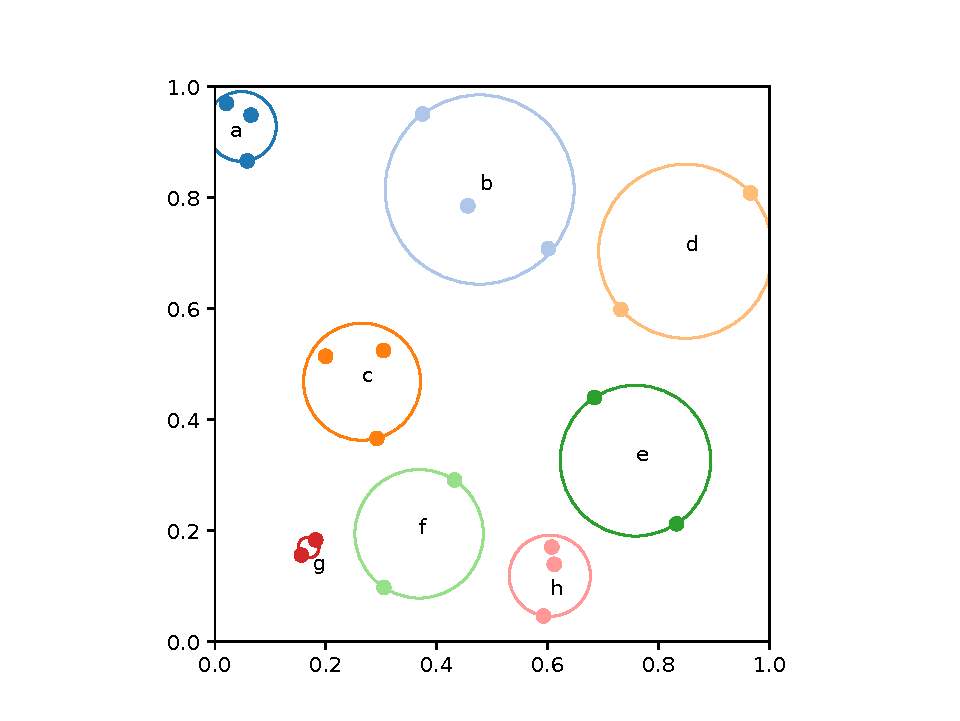
\includegraphics[width=0.4\textheight]{obrazky-figures/balltree/full_balltree.pdf}
    \caption{Grafické znázornění listových uzlů vybudovaného stromu pro $m = 3$.}
\end{subfigure}
\hfill
\begin{subfigure}[t]{0.45\columnwidth}
    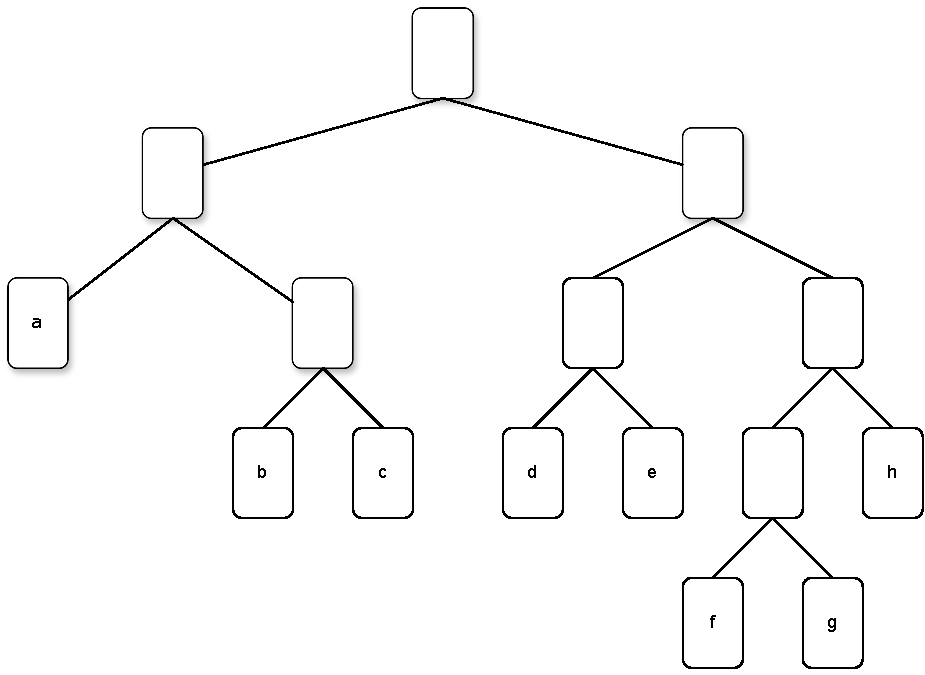
\includegraphics[width=0.3\textheight]{obrazky-figures/balltree/diagram_balltree.drawio.pdf}
    \caption{Grafické znázornění stromu balltree.}
\end{subfigure}
\caption{Grafické znázornění balltree, jak v~prostorovém zobrazení (pouze listové uzly), tak ve formě stromového diagramu.}
\label{fig:balltree_done}
\end{figure}

\subsubsection{Výhody a nevýhody}
Velkou výhodou je, že struktura se nemění s~rostoucím množstvím dimenzí $p$. Pro nižší počet (např. $p=3$) dimenzí je balltree pomalejší než např. KD-tree, ale u~mnoho dimenzionálních prostor je balltree rychlejší \cite{knn-survey}. Balltree je rovněž zatížen prokletím dimensionality.



\subsection*{Další prostorové struktury}
Mimo zmíněné struktury existuje i mnoho dalších struktur, které mohou, ale i nemusejí být založeny na výše jmenovaných. Některé různými způsoby pozměňují výše jmenované, jako například přidání různých heuristik aplikovaných na výstavbu. Struktury je možné optimalizovat na paměťovou náročnost, dobu potřebnou k~výstavbě struktury, dobu potřebnou pro vyhledání prvního, ale obecně jakéhokoliv souseda. Dále pak může být struktura zaměřena na mnoho dimenzionálních prostor, kde se řeší efektivita výstavby, ale i vyhledávání v~ní \cite{reviewNN}.

\section{Optimalizace na strojové úrovni}
V~prezentovaných strukturách je často potřeba vypočítávat hodnotu podle nějakého konkrétního vztahu hned pro několik hodnot. V~těchto případech se jedná o~smyčku, která se postupně vykonává nad všemi daty, u~kterých to je potřeba. Moderní procesory však umožňují používat instrukce typu \emph{Single Instruction Multiple Data} (SIMD) česky, jedna instrukce více dat, což jsou instrukce rozšiřující možnosti procesoru o~další instrukce, které umožňují některé operace vykonávat najednou paralelně nad více daty. Obvykle přidávají i další registry, aby byla práce s~více daty vůbec možná. Existuje více instrukčních sad, které umožňují různé a různě datově široké operace, jako například SSE a různé verze AVX. Například na architektuře ARM se mluví o~SVE, Helium nebo Neon \cite{ARM_helium,ARM_Neon,ARM_SVE}. Porovnání těchto architektur je v~tabulce \ref{tab:simd_comparison}.

\subsection*{Vektorizace}
Jak je uvedeno výše, tak existuje mnoho instrukčních sad, které mezi sebou nemusejí být kompatibilní. Stěžejní je velikost registrů, se kterou dokážou pracovat a operace co dokážou vykonávat.

\subsubsection{Vektorizace pomocí překladače}
Dnešní překladače jsou natolik inteligentní, že samy o~sobě provádějí vektorizaci pokud dokážou detekovat, že to má smysl a že to jde. Obvykle však překladače neprovádějí tuto optimalizaci v~základním nastavení. Je třeba si jej vynutit přepínačem jako například u~překladače \emph{GCC} (GNU Compiler Collection) pomocí:
\begin{itemize}
    \item -ftree-vectorize: tento flag povoluje vektorizaci kódu.
    \item -march=native: tento flag informuje překladač o~cílové instrukční sadě procesoru.
    \item -ffast-math: tento flag povoluje agresivnější optimalizace, které mohou zahrnovat vektorizaci.
    \item souhrný přepínač \emph{-o3}, který aktivuje další optimalizace.
\end{itemize}


Bohužel, překladače neumí vektorizovat všechno. Obecně se dá říci, že čím složitější kód, tím je menší šance, že překladač rozpozná možnost k~vektorizaci. Programátor může překladači pomoci a dát mu tzv. nápovědy přímo do kódu např. ohledně aliasingu\footnote{Označení pro situaci, kdy mají respektive nemají dva ukazatele plně nebo částečně stejné cíle \cite{intel2023autovectorization}.}, očekávaného počtu opakování smyčky, zarovnání v~paměti nebo zakázání vektorizace pro nějakou sekci \cite{gcc_tree_ssa_vectorization}.


\subsubsection{Ruční vektorizace}
Pokud je kód více komplexní nebo programátor nechce spoléhat na překladač a nebo věří, že dokáže vektorizaci udělat lépe, je možné provést vektorizaci ručně \cite{gcc_vector}, což může být docela náročná činnost. Nejnáročnější může být příprava dat. Data je potřeba správně připravit do správných registrů příslušné velikosti. Je potřeba mít na paměti, že tato příprava dat musí být co možná nejefektivnější.

Je tedy logické a vhodné, aby kód byl strukturován už s~myšlenkou na to, že bude použita optimalizace vektorizací. Bohužel často může dojít k~tomu, že je potřeba implementovat, jak SIMD verzi výpočtu tak i sériovou verzi, protože obvykle je potřeba, aby byly hodnoty se kterými se počítá násobkem osmi, čtyř podle typů hodnot a verze SIMD. U~AVX s~256 bitovými registry a počítání s~4 bytovými floaty je nutné, aby počet hodnot odpovídal násobkům osmi.

Pro příklad je možné si představit pole hodnot, kde je potřeba vynásobit konstantou každou hodnotu. V~sériovém provedení bude for cyklus procházet prvek po prvku a každou hodnotu vynásobí, což jde vidět na kódu \ref{code:c_const_mult}.

U~implementace používající AVX bude potřeba si připravit registr, kde bude mít osmkrát vedle sebe konstantu, kterou se budou násobit všechny prvky. Dále pak je nutné zkopírovat prvky, které je potřeba vynásobit. A~následně je potřeba hodnoty zkopírovat zpět do pole odkud jsou data brána. V~jeden okamžik je vypočítáno osm hodnot. Je tedy teoreticky 8x rychlejší. Násobení je znázorněno na obrázku \ref{fig:AVX_ilustration}. V~realitě tomu tak obvykle však není kvůli přípravám. Další zpomaleni může nastat pokud vstupní pole neobsahuje násobek osmi prvků. S~tím je možné se vypořádat tzv. \uv{dokročením} sériovou alternativou nebo kopírováním 8 míst z~paměti (i když už neobsahují validní data) a následně zkopírovat do výsledku pouze hodnoty, které nesou význam. Jak by mohlo takové násobení pole konstantou vypadat, je možné vidět v~kódu \ref{code:c_const_avx}.

\begin{figure}
    \centering
    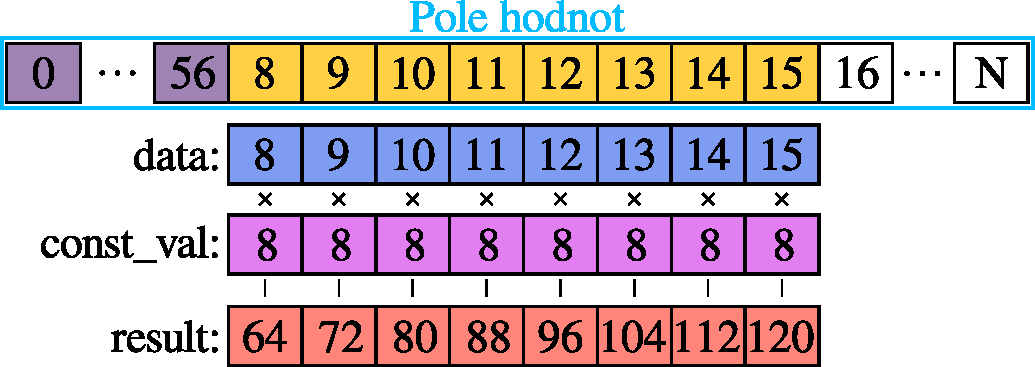
\includegraphics[scale=0.8]{obrazky-figures/avx/AVX_ilustration.pdf}
    \caption{Ilustrace fungování násobení velkého pole konstantou $8$. Na obrázku je vidět vstupní pole, které zároveň slouží jako výstupní. Pole obsahuje čísla od nuly po $N$ uspořádaná zleva doprava. Na obrázku je znázorněna situace, kdy prvních 8 prvků pole bylo již vynásobeno. Zkopírované prvky (označené žlutou barvou) se nacházejí v~registru pojmenovaném \uv{data}, který je označen modrou barvou. Další registr, \uv{const\_val} (označený růžovou barvou), obsahuje osmkrát opakovanou konstantu $8$. Ve finálním registru \uv{result} je uložen výsledek násobení (znázorněn červenou barvou). Tento výsledek by poté byl kopírován zpět do původního pole, do žlutě označené sekce pole. Proces násobení by následně pokračoval posunem o~8 prvků doprava, tedy na hodnoty od 16 do 23. }
    \label{fig:AVX_ilustration}
\end{figure}



Vhodné je, aby struktury byly uloženy jako struktury polí, nikoliv jako pole struktur. Pokud tomu tak není, může to vést k~značnému zpomalení, jenž může dosti zneefektivnit takto naimplementovaný výpočet.  

Je zjevné, že u~některých algoritmů není možné nebo není výhodné použít SIMD zpracování dat. Může to být buď způsobeno nekompatibilitou algoritmu nebo nepřipraveným návrhem uložení dat pro tento styl zpracování.

\begin{lstlisting}[language=C, label={code:c_const_mult}, caption=Ukázka funkce pro násobení pole konstantou v~jazce C.]
    void multiplyByConst(float *f, float c, int n){
        for (size_t i = 0; i < n; i++){
            f[i] = f[i]*c;
        }
    }
\end{lstlisting}

\begin{lstlisting}[language=C,label={code:c_const_avx}, caption=Ukázka funkce pro násobení pole konstantou pomocí AVX instrukcí. Ilustrace takového násobení je znázorněna na obrázku \ref{fig:AVX_ilustration}.]
    void multiplyByConstAVX(float *f, float c, int n){
        __m256 const_val = _mm256_set1_ps(c);
        size_t i;
        for (i = 0; i + 7 < n; i += 8) {
            __m256 data = _mm256_loadu_ps(&f[i]);
            __m256 result = _mm256_mul_ps(data, const_val);
            _mm256_storeu_ps(&f[i], result);
        }
        multiplyByConst(f+i, c, n-i);

    }
\end{lstlisting}


\begin{table}[h!]
\centering
\begin{tabular}{| >{\raggedright\arraybackslash}p{3.2cm} | >{\centering\arraybackslash}p{2.2cm} | >{\centering\arraybackslash}p{2.2cm} | >{\centering\arraybackslash}p{2.2cm} | >{\centering\arraybackslash}p{2.2cm}  |}
\hline
\textbf{Parametr} & \textbf{AVX/AVX2} & \textbf{ARM Helium} & \textbf{AVX-512} & \textbf{ARM Neon}  \\
\hline
Šířka vektoru & 256-bit & 128-bit & 512-bit & 64-bit až 128-bit \\
\hline
Počet registrů & 16 YMM registrů & 32 & 32 ZMM registrů & 16-32 \\
\hline
Datové typy &  Int (8,16,32,64),  Float, Double & Int, Float,  & Int (8,16,32,64),  Float(32,16),  Double & Int (8,16,32,64), Float  \\
% \hline
% Podpora instrukcí & FMA, Permute & MVE instrukce & Široký rozsah, včetně nových redukčních a konfliktních instrukcí & SIMD operace \\
\hline
Architektura & x86\_64 & ARMv8.6-A a novější & x86\_64 & ARMv7 a novější \\
\hline
\end{tabular}
\caption{Srovnání SIMD instrukcí: AVX/AVX2, ARM Helium, AVX-512 a ARM Neon.}
\label{tab:simd_comparison}
\end{table}
\newpage









\chapter{Koncept struktury řešící problém nejbližšího souseda}
\label{koncept}

Tato práce reimplementuje verzi algoritmu nejbližšího souseda, popsanou v~práci \uv{Almost constant-time 3D nearest-neighbor lookup using implicit octrees} \cite{octreehash}. Zmíněná implementace kombinuje použití struktur octree a hašovací tabulky spolu s~využitím vlastností Voronoi diagramu s~tím, že tato implementace je rozšířena pro vyhledávání orientovaných bodů.

Octree je vystavěný klasickým způsobem popsaným v~sekci \ref{octree} nad Voronoi diagramem při dodržení kriteria pro maximální množství zasahujících Voronoi buněk do jednoho oktetu. Zde přichází ta nejzajímavější část této struktury. Postupně jsou procházeny jednotlivý uzly vystavěného stromu a ty jsou umístěny do hašovací tabulky.
\section{Model struktury}
Struktura se staví ve 3 fázích, které je možné vidět na obrázku \ref{fig:struct-model}. Fáze probíhají postupně a po vybudování celé struktury se interaguje pouze s~hašovací tabulkou a skrz ní se stromem.

\begin{figure}
    \centering
    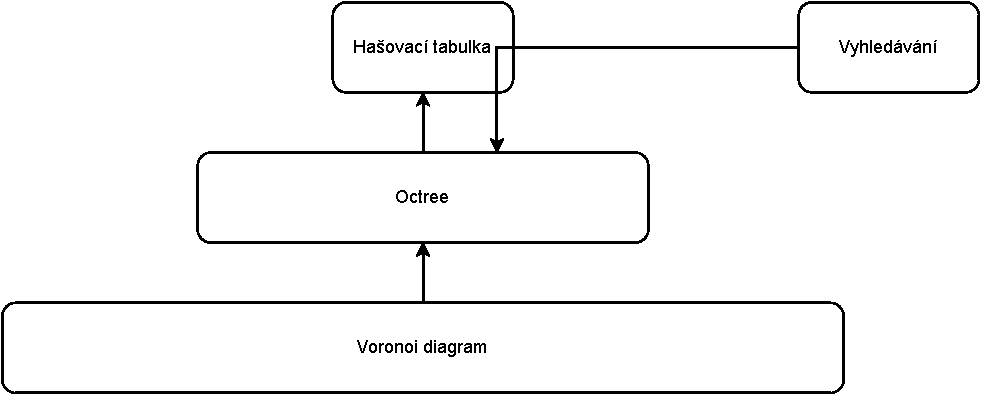
\includegraphics[scale=0.5]{obrazky-figures/octree/structu_diagram.pdf}
    \caption{Ilustrační schéma prezentované struktury. Na první úrovni je vystavěn Voronoi diagram, nad ním je vystavěn octree a nad ním je vystavěna hašovací tabulka. }
    \label{fig:struct-model}
\end{figure}

\subsection*{Index hašovací tabulky}
Index se skládá ze dvou částí. První částí je identifikace sektoru. Identifikace sektoru může být trojice\footnote{Pro $p=3$ pro $p=2$ stačí dvojice.}, kde každá složka odpovídá souřadnici v~jedné dimenzi. Druhou složkou je úroveň ve stromu. Tato dvojice jednoznačně identifikuje jakýkoliv uzel ve stromu. To jakým způsobem funguje souřadnice je zachyceno na~obrázcích \ref{fig:coordinates-octree} a \ref{fig:hashtable_octree}, na nichž je znázorněn vztah mezi hašovací tabulkou, indexy v~ní a octree.

\begin{figure}
    \centering
    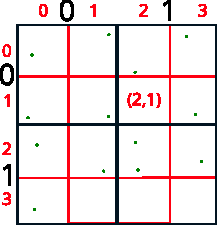
\includegraphics[scale=1.3]{obrazky-figures/hashtree/diagram_idx_prostory.pdf}
    \caption{Identifikace sektorů v~quadtree (pro octree by situace vypadala podobně, jen by indexy nebyly dvojice ale trojice.), černě jsou znázorněny indexy na vyšší úrovni. Červeně pak ty na nižší úrovni. Na obrázku lze vidět i dokonce, jak by byl indexován jeden z~červených sektorů.}
    \label{fig:coordinates-octree}
\end{figure}

\begin{figure}
    \centering
    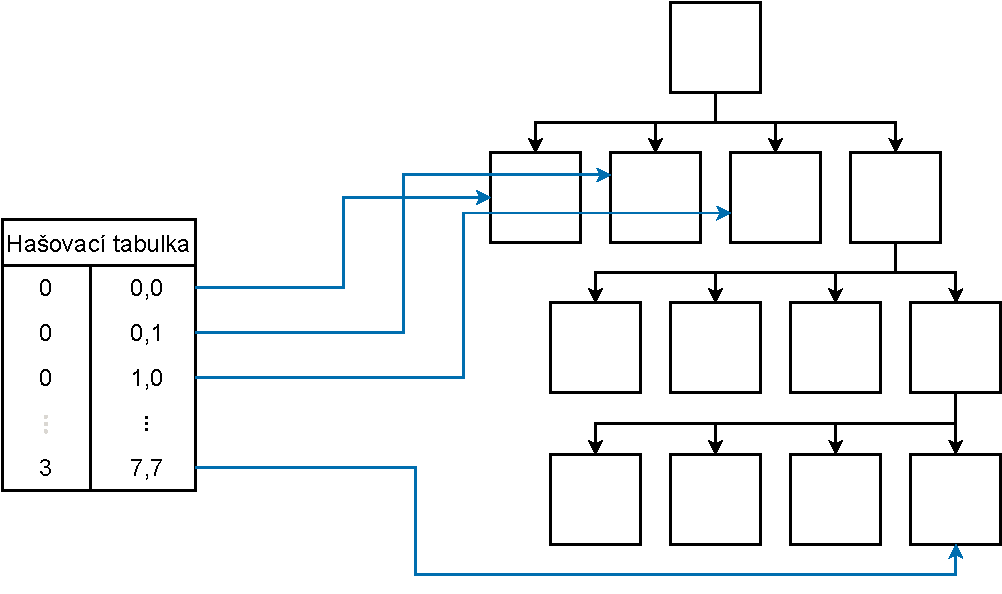
\includegraphics[scale=.8]{obrazky-figures/hashtree/hashtable_octree.pdf}
    \caption{Zobrazení souvislosti mezi hašovací tabulkou, indexy a octree (quadtree). Modrou barvou jsou znázorněny odkazy z~hašovací tabulky do quadtree. Indexy hašovací tabulky jsou ve dvou sloupcích, kde první sloupec je úroveň znázornění a druhý je identifikátor sektoru (viz obrázek \ref{fig:coordinates-octree}). V~obrázku se nachází jen část podstromu a hašovací tabulky.}
    \label{fig:hashtable_octree}
\end{figure}

Úroveň stromu určuje limity, které souřadnice mají, přesněji řečeno od nuly\footnote{Předpokládá se indexování od nuly.} po \(2^l-1\) je maximální hodnota, která se může objevit, kde \(l\) je úroveň.

\subsection*{Složitost}
Pokud by vyhledávání probíhalo jen ve stromu, byla by složitost logaritmická. Nicméně prezentovaná struktura nad tímto stromem vystaví hašovací tabulku, ve které probíhá binární vyhledávání, čímž se složitost sníží na logaritmicky logaritmickou \cite{octreehash}. 


\subsection*{Vyhledávání}
Vyhledávání využívá princip binárního vyhledávání, které má logaritmickou složitost. Proces nalezení zahrnuje binární prohledávání prostoru určeného souřadnicemi uzlu v~hašovací tabulce, což umožňuje efektivně získat přístup k~odpovídajícím uzlům. Tento přístup je  efektivní v~kombinaci s~hašovací tabulkou, která umožňuje rychlé získání dat bez nutnosti procházet celý strom.

Nechť \( p \) je vyhledávaným bodem, \( l_{\text{min}} \) je minimální úroveň ve stromu a \( l_{\text{max}} \) je maximální úroveň. Potom existuje i \( l_c \). Dále pak existuje hašovací tabulka \( H \), která pro index vrací buď \( \text{null} \) v~případě, že neexistuje prvek pod takovým indexem, nebo vrátí uzel stromu. Potom také existuje funkce \( \text{find\_idx()} \), která pro vstupní bod a úroveň ve stromu vrátí souřadnice sektoru, ve kterém se bod \( p \) nachází.
\begin{enumerate}
    \item Pokud \( l_{\text{max}} - l_{\text{min}} \) je roven 1, vyhledávání se zastaví a nejbližší soused se nachází v~\( l_{\text{max}} \). Jinak se pokračuje dále.
    \item \( l_c = \frac{l_{\text{max}} - l_{\text{min}}}{2} \), \( \text{idx} = \text{find\_idx}(l_c, p) \).
    \item Pokud \( H(l_c, \text{idx}) \) je roven \( \text{null} \), vyhledávání pokračuje s~\( l_{\text{max}} = l_c \) a \( l_{\text{min}} \) zůstane nezměněný. V~opačném případě vyhledávání pokračuje s~\( l_{\text{min}} = l_c \) a \( l_{\text{max}} \).
\end{enumerate}

Pomocí tohoto způsobu je nalezen uzel, ve kterém se nachází nejbližší soused. Nalezení nejbližšího souseda je už jen otázkou iterace skrz všechny prvky tohoto uzlu. 

\subsection*{Vyhledání $k$-nejbližších sousedů}
Algoritmus pro nalezení k-nejbližšího souseda je velmi podobný jako u~nejbližšího souseda. Po nalezení uzlu hašovací tabulkou jsou prvky seřazeny a je vrácena seřazená sekvence. Pokud je potřeba víc prvků než je v~uzlu, algoritmus provede stejný postup nad otcovským uzlem.

\subsection*{Vyhledávání podle normály}

Vyhledání je typicky omezeno vzdáleností. Po určení uzlu hašovací tabulkou je nalezen nejvzdálenější bod v~seznamu bodů. Pokud je maximální vzdálenost menší než nastavená maximální vzdálenost, a pokračuje se ve vyhledávání nejvzdálenějšího bodu v~otcovském uzlu. Je nutné pokračovat dokud není nalezen prvek, co je dál než je požadováno. V~takovém případě je v~tomto uzlu i nejvzdálenější prvek, který je potřeba vzít v~potaz. Nejvzdálenější prvek splňujícím zadání je nalezen a určí množinu prvků. Z~této množiny je vybrán ten s~nejpodobnější normálou. 

\subsubsection{Orientovaný bod}
Tato práce implementuje bod jako orientovanou strukturu. Takový bod krom své souřadnice obsahuje i další trojici, která určuje jeho směr. Tento směr je jednotkový vektor a slouží pouze k~určení směru. Pomocí goniometrie je možné porovnávat takové směry.


\section{Konkrétní příklad vyhledávání}
Nechť existuje bod \( E \), pro který je potřeba nalézt nejbližšího souseda. Předpokládá se existence vybudované struktury tak, jak je na obrázku \ref{fig:vyhledávání}, ve které se bude vyhledávat.

\begin{enumerate}
    \item \( l_{\text{min}} = 0 \) a \( l_{\text{max}} = 3 \), tím pádem \( l_c = 2 \). V~hašovací tabulce se pokusí nalézt uzel pod indexem \( (2, \text{find\_idx}(E,2)) \), což vyústí v~navrácení hodnoty \( \text{null} \), tento neexistující uzel je znázorněn ve stromu zelenou barvou.
    \item \( l_{\text{min}} = 0 \) a \( l_{\text{max}} = 2 \), tím pádem \( l_c = 1 \). V~hašovací tabulce se pokusí nalézt uzel pod indexem \( (1, \text{find\_idx}(E,1)) \), což skončí úspěchem v~podobě nalezeného uzlu (v~obrázku \ref{fig:vyhledávání} znázorněno oranžovou).
    \item \( l_{\text{max}} - l_{\text{min}} = 1 \), nejbližší soused se nachází v~tomto uzlu.
    \item Jsou postupně otestovány všechny prvky na vzdálenost k~\( E \) a tím je nalezen skutečně nejbližší soused.
\end{enumerate}

\begin{figure}
\centering
\begin{subfigure}[t]{\columnwidth}
    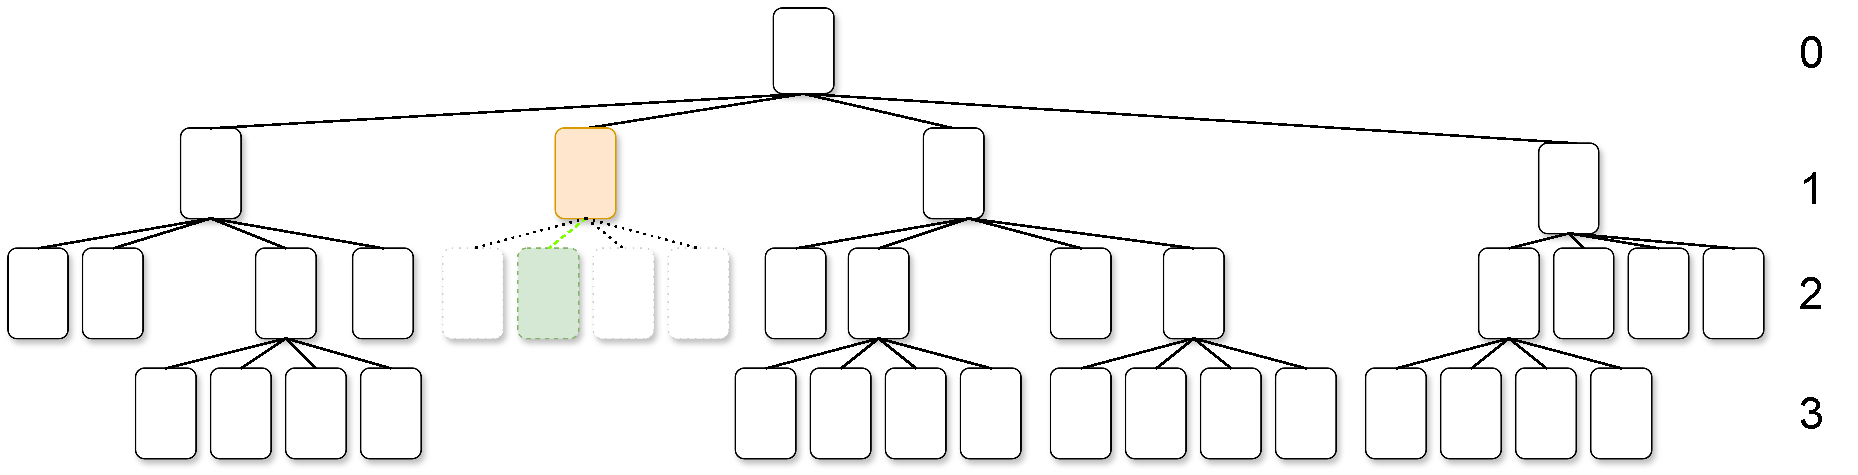
\includegraphics[width=0.67\textheight]{obrazky-figures/hashtree/octreehash_search_treeview.drawio.pdf}
    \caption{Grafické znázornění stromu. Přerušovaně jsou znázorněny neexistující uzly, jejichž neexistence ovlivňuje vyhledávání (ten hlavní je znázorněn zelenou barvou). Oranžovou barvou je znázorněn uzel, ve  kterém se nachází nejbližší soused. Po pravé straně jsou k~nalezení úrovně stromu.}
\end{subfigure}
\hfill
\begin{subfigure}[t]{\columnwidth}
\centering
    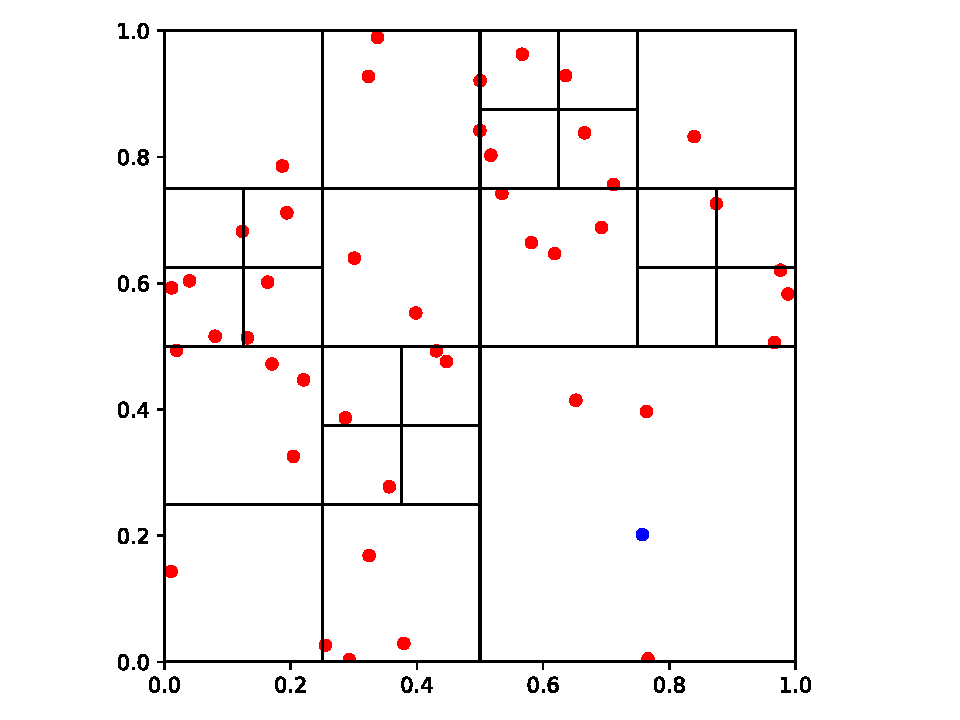
\includegraphics[width=0.4\textheight]{obrazky-figures/hashtree/hashtree-search-octview.pdf}
    \caption{Grafické znázornění stromu v~podobně diagramu. K~modrému bodu je vyhledáván nejbližší soused.}
\end{subfigure}
    \caption{Ilustrační obrázek demonstrující vyhledávání.}
    \label{fig:vyhledávání}
\end{figure}



\section{Testovací kritéria}
Pro účely ověření funkčnosti a rychlosti struktury je potřeba ji podrobit testům. V~této kapitole jsou definovány metriky, které byly při testech aplikovány a zkoumány.

\subsection*{Testování přesnosti}
Pro testování přesnosti byla vytvořena co možná nejjednodušší implementace, která využívá počítání hrubou silou. Ta dostane jako vstup množinu $R$ náhodných bodů pro množinu sousedů a $T$ náhodných bodů jako množinu testovaných bodů. Dále pak se předpokládá existence $K$, což je počet sousedů, který bude implementovaný algoritmus vyhledávat. Následně budou vypočítány seznamy pro každý z~testovaných bodů obsahující seřazené posloupnosti vzhledem ke vzdálenosti k~jednomu bodu z~$T$. Výpočet for cyklem prochází body z~testovací množiny a pomocí \emph{std::sort()} ze standardní knihovny C++ je seřazen podle vzdálenosti k~testovanému bodu a seznam je uložen do souboru tak, aby nebylo potřeba jej počítat pro každý test. Tímto způsobem budou spočítány seřazené posloupnosti pro všechny body z~$T$.

V~další fázi se jen porovnají prvky vygenerované z~naprogramované implementace a implementace hrubou silou. Je potřeba mít na paměti, že všechny body včetně vzdáleností jsou počítány na přesnosti datového typu float. V~případě, že prvky z~množin jsou rozdílné, tak jsou ještě porovnány vzdálenosti k~testovanému bodu (na přesnosti float). Pokud jsou stejné, předpokládá se, že algoritmus pracuje správně.

\subsubsection*{První nejbližší soused}
Pro kontrolu fungování nejbližšího souseda bude využita vypočtená množina tak, jak je popsaná výše s~tím, že se porovnává jen první prvek.

\subsubsection*{$K$-tý nejbližší soused}
Ačkoliv autoři původního článku vůbec tuto strukturu netestují pro k-NN, tak by struktura měla fungovat i pro tento případ. Pro ověření bude využita množina tak, jak je popsána výše.

\subsubsection*{První nejbližší soused s~nejpodobnější normálou}
Pro vyhledávání podle normály bude použit podobný přístup. S~tím rozdílem, že bude vypočítáno jen nejlepších 10 bodů. Těchto 10 bodů se spočítá hrubou silou. Jedná se o~10 nejlépe orientovaných z~množiny bodů s~fixní vzdáleností. 


\subsubsection*{Výstupy testů}
Ve všech testech se bude sledovat množství úspěšných vyhledání (nalezen stejný prvek jako v~kontrolní implementaci) a v~případě, že vyhledání nalezne jiný bod než ten správný podle kontrolní implementace, tak je spočten rozdíl vzdáleností od hledaného bodu a ten je zprůměrován pro získání průměrné odchylky, kterou struktura vytváří.



\subsection*{Testování výkonu}
Při testování struktury určené k~vyhledávání nejbližšího souseda je potřeba sledovat následující metriky:
\begin{enumerate}
    \item Doba výstavby stromu.
    \item Množství potřebných uzlů stromu.
    \item Doba potřebná pro vyhledání prvního souseda a vyhledání $n$-tého souseda.
    \item Kriterium $M_{max}$, tedy kolik Voronoi buněk maximálně zasahuje do uzlu.
\end{enumerate}

Následující metriky bude potřeba sledovat v~několika různých podmínkách, především pak vstupní rozdělení bodů. Výkon algoritmů nejbližšího souseda může značně ovlivnit právě rozdělení bodů. Jmenovitě: rovnoměrné náhodné rozdělení a body tvořící plochy.


\begin{figure}
\begin{subfigure}[t]{0.49\columnwidth}
\centering
    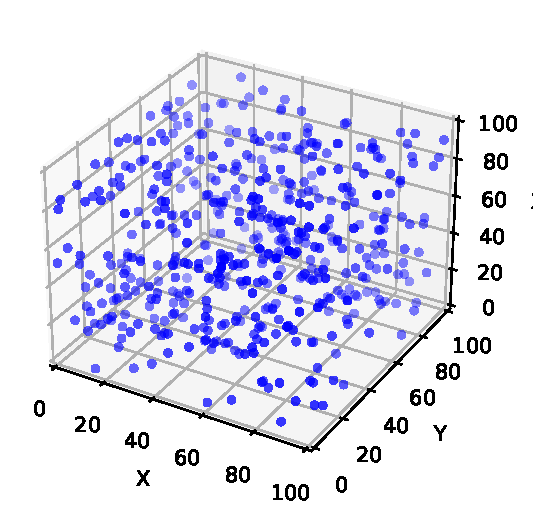
\includegraphics[scale=0.5]{obrazky-figures/testing/randompoints.pdf}
    \caption{Náhodné rozdělení bodů.}
\end{subfigure}
\hfill
\begin{subfigure}[t]{0.49\columnwidth}
\centering
    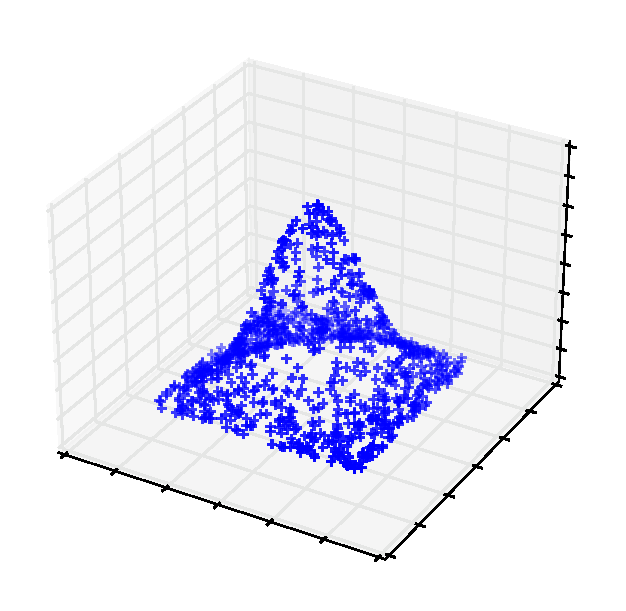
\includegraphics[scale=0.45]{obrazky-figures/knn_norm/points_3d normal_plane_1000.pdf}
    \caption{Plocha tvořena body.}
\end{subfigure}


\caption{Ukázka náhodného rozdělení bodů použitých v~testech. Charakteristiky jsou převzaty ze \cite{octreehash}.}
\end{figure}



\subsection*{Degenerativní případy}
Autoři studie zmiňují, že struktura může mít problémy se zpracováním oblastí, které vytvářejí Voronoi buňky tak nešťastně, že spolu sousedí hned několik v~jednom místě. Jak to může vypadat lze vidět na obrázku \ref{fig:degenerative_case}. Tyto případy nebudou testovány, protože nejsou pro tuto strukturu vhodné.




\begin{figure}
\centering
\begin{subfigure}[t]{0.4\columnwidth}
    \centering
    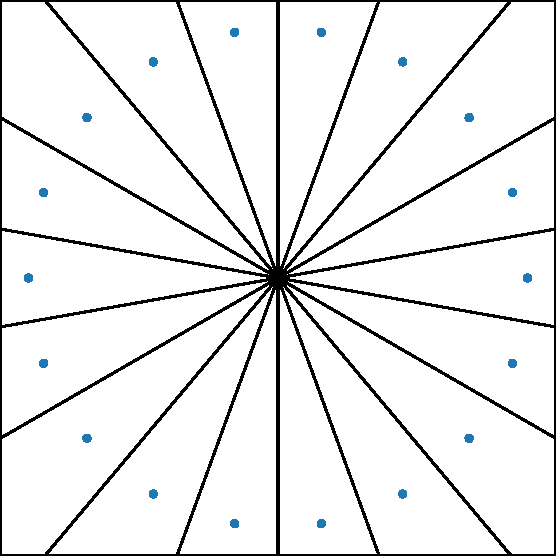
\includegraphics[scale=0.45]{obrazky-figures/testing/circletest.pdf}
    \caption{Body uspořádané do kruhu a Voronoi diagram nad nimi.}
\end{subfigure}
\hfill
\begin{subfigure}[t]{0.45\columnwidth}
    \centering
    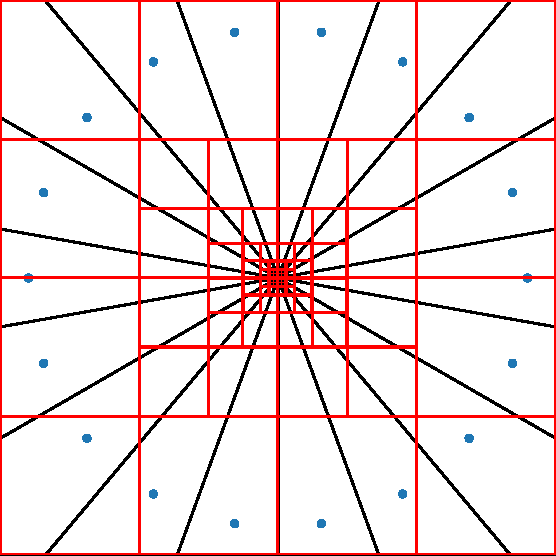
\includegraphics[scale=0.45]{obrazky-figures/testing/circletest_part2.pdf}
    \caption{Rekurzivní dělení se nikdy nezastaví protože, podmínka je množství zasahujících Voronoi buněk do čtverce, což u~čtverců v~blízkosti středu nemusí nikdy nastanou.}
\end{subfigure}
    \caption{Ukázka nevýhodného rozdělení bodů v~$p=2$ prostoru. Všechny Voronoi buňky mají jedno místo, kde se dotýkají.  }
    \label{fig:degenerative_case}
\end{figure}


















\chapter{Implementace rychlé varianty algoritmu nejbližšího souseda}


\begin{figure}
    \centering
    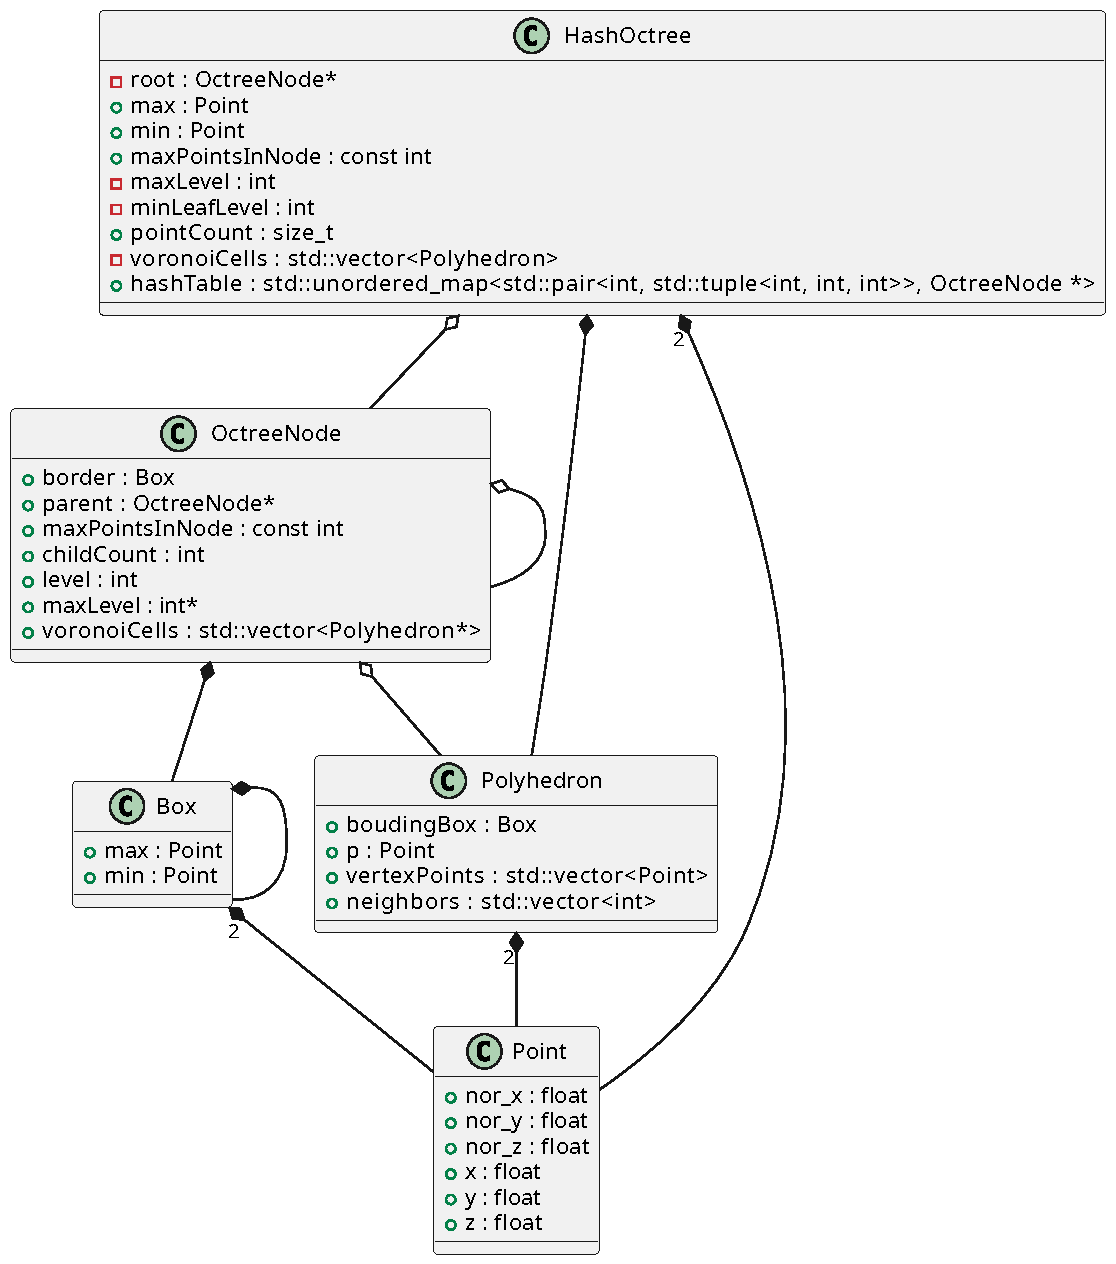
\includegraphics[scale=0.8]{obrazky-figures/hashtree/uml.pdf}
    \caption{UML diagram klíčových členů, klíčových struktur.}
    \label{fig:uml}
\end{figure}

Výstavba struktury je rozdělena do několika fází, které na sobě závisí. Výsledkem je struktura skládající se z~octree a hašovací tabulky, která se odkazuje na uzly této tabulky.

\section{Struktury použité v~implementaci}
Přehled vybraných klíčových použitých struktur při implementaci je možné vidět na obrázku~\ref{fig:uml}.

\subsection*{OctreeNode}
Tato struktura slouží k~skladování informací a potomků uzlů stromu. Každý uzel může mít až osm poduzlů, které jsou skladovány v~poli ukazatelů, kde $null$ indikuje neexistenci syna. Každý uzel má odkaz na svého otce, což usnadňuje navigaci ve stromu od listových uzlů. Důležité je také pole skladující všechny Voronoi buňky zasahující do prostoru vymezujícího tento uzel. V~neposlední řadě jsou zde čísla ukládající informace používané při výstavbě stromu, hašovací tabulky nebo při vyhledávání. Vše je shrnuto v~obrázku \ref{fig:uml} včetně závislosti na jiných třídách.

\subsection*{Hashtree}
Třída Hashtree obaluje celou strukturu. Obsahuje všechny Voronoi buňky, na které se odkazují všechny uzly stromu. Dále obsahuje kořenový uzel struktury, hašovací tabulku a další.

\subsection*{Polyhedron}
Třída reprezentuje mnohostěn a protože Voronoi buňky jsou mnohostěny, jsou použity pro jejich reprezentaci. Obsahuje seznam vrcholů a středový bod, který určuje tento mnohostěn (Voronoi buňku). Údaje pro konstrukci jsou získány ze struktury vypočítané pomocí knihovny voro++ (viz sekce zabývající se Voronoi diagramem \ref{Voroni_imp}), protože struktura z~voro++ nese zbytečně mnoho dalších informací, které jsou irelevantní pro použití v~této aplikaci.

\subsection*{Box}
Box je jednoduchá struktura pro ukládání krychlí. Je definována dvěma souřadnicemi. Klíčové u~této třídy jsou především metody zpřehledňující implementaci.

\subsection*{Point}
Struktura pro skladování bodu společně s~normálou. Je implementována pro zpřehlednění zápisu.

\section{Implementace výstavby stromu}
Veškerá implementace je skryta pod třídou \emph{Hashtree}. Hashtree reprezentuje kompletní strukturu jako celek a nabízí metody pro vyhledávání. Všechny body jsou nahrány najednou jako vstupní pole hodnot, třída mimo to očekává hranice, kde se body nacházejí, tedy vlastně krychli ohraničující všechny body. Další parametr konstruktoru je počet jader, který má být použit pro výstavbu a v~neposlední řadě i cílové kritérium, které určuje maximální množství Voronoi buněk, zasahujících do listového uzlu.

Konstruktor potom přistoupí k~první fázi a to je výpočet Voronoi diagramu. Druhou fází je stavba octree nad Voronoi diagramem. Poslední fází je umístění prvků do hašovací tabulky.

\subsection*{Voronoi diagram}
\label{Voroni_imp}
Pro výstavbu octree je nezbytné vypočítat Voronoi diagram. Pro výpočet Voronoi diagramu je využitá knihovna voro++ \cite{voro,voro_para}, která umožňuje počítat Voronoi rozdělení paralelně na CPU. Knihovna nejdříve vyžaduje inicializaci prostoru podle krychle ohraničující prostor a dále vyžaduje body na kterých vytváří diagram. Následně jsou ve smyčce vypočítány všechny Voronoi buňky, ze kterých jsou extrahovány jen ty důležité informace do struktury \emph{Polyhedron}.

 Autoři původní implementace nezmiňují, jakým způsobem počítají Voronoi buňky. Vzhledem k~časů uvedených ve studii potřebných pro stavbu struktury, ale pravděpodobně používají nějakou přesnější metodu výpočtu. Knihovna voro++, počítá voronoi buňky na datovém typu double, ten je však přetypován při vkládání do struktury \emph{Polyhedron} na float kvůli rychlejším výpočtům později.

\subsection*{Výstavba stromu}

Pro výstavbu stromu je implementovaná speciální struktura \emph{OctreeNode}, která reprezentuje jeden uzel stromu. Po dokončení výpočtu Voronoi buněk je vytvořen kořenový uzel, jenž dostane na vstupu všechny mnohostěny a meze celého zadaného prostoru. Rekurzivním přístupem je vybudován strom, který o~každém z~mnohostěnů rozhodne, zda se nachází v~právě prozkoumávané krychli\footnote{Zkoumají se jen ty mnohostěny, co patřily do nadřazeného uzlu.}. Při rozdělení prostoru na osminy jsou zkontrolovány všechny Voronoi buňky, které náležely otci. Rekurzivní výstavba stromu bude pokračovat až do okamžiku, kdy počet Voronoi buněk zasahujících do sledované krychle nebude menší nebo roven jako stanovené maximum.

Nejnáročnější část výstavby stromu je kontrola náležitostí mnohostěnu do uzlu stromu. V~implementaci se kombinuje několik přístupů. Využívá se toho, že detekovat, zda je nějaký bod konvexního tvaru uvnitř krychle, je snadné. Je zjevné, že pokud alespoň jeden bod konvexního tvaru je uvnitř krychle, musí to nutně znamenat, že ona krychle a mnohostěn jsou v~kolizi (obrázek \ref{fig:colision_approx_vertex}). Poslední detekční mechanismus je algoritmus GJK, který se však používá pouze, pokud bounding box zkoumané Voronoi buňky je v~kolizi se zkoumanou krychlí. Postup je znázorněn algoritmem \ref{algo:detection-polyhedron} a taktéž je možné jednotlivé přístupy vidět na obrázku \ref{fig:colision_approx}.

Nechť existuje funkce \emph{isInside()}, která má na vstupu krychli a dále pak množinu nebo jeden bod a vrátí $true$, pokud alespoň jeden z~bodů nebo samotný bod je uvnitř dané krychle. Algoritmus použitý v~implementaci vypadá takto:

\begin{figure}
\begin{subfigure}[t]{0.29\columnwidth}
    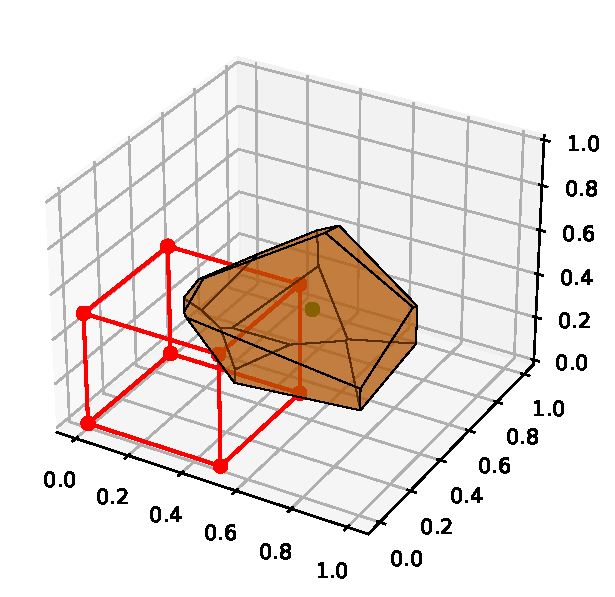
\includegraphics[scale=0.5]{obrazky-figures/hashtree/center_point.pdf}
    \caption{Kontrola středového bodu Voronoi buňky zda se nachází uvnitř krychle.}
    \label{fig:colision_approx_center}
\end{subfigure}
\hfill
\begin{subfigure}[t]{0.29\columnwidth}
    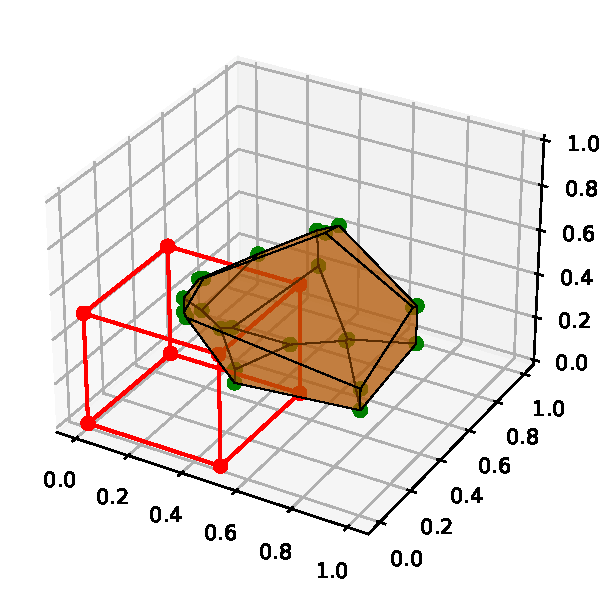
\includegraphics[scale=0.5]{obrazky-figures/hashtree/vertex_box.pdf}
    \caption{Kontrola zda jeden z~vrcholů Voronoi buňky je uvnitř krychle. Vrcholy Voronoi buňky jsou znázorněny zelenou barvou.}
    \label{fig:colision_approx_vertex}
\end{subfigure}
\hfill
\begin{subfigure}[t]{0.29\columnwidth}
    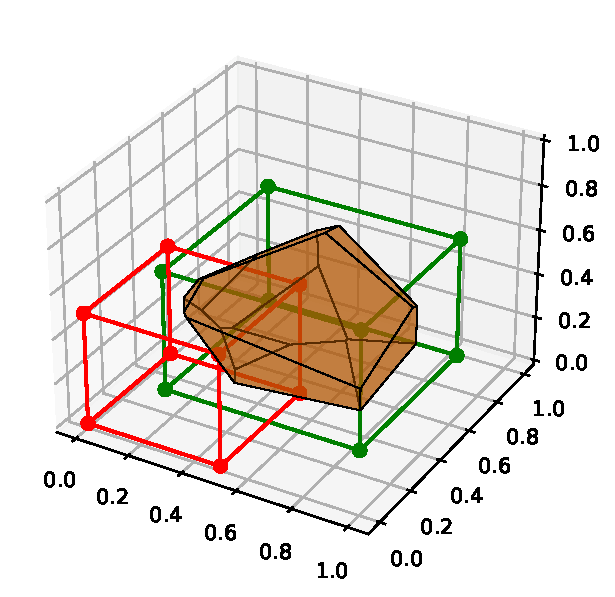
\includegraphics[scale=0.5]{obrazky-figures/hashtree/bouding_box.pdf}
    \caption{Kontrola zda jeden z~vrcholů blending boxu Voronoi buňky je uvnitř krychle. Bounding box je znázorněn zeleně.}
    \label{fig:colision_approx_bb}
    
\end{subfigure}

    \caption{Grafické znázornění různých přístupů při zjišťovaní kolizí. Červenou barvou je znázorněna právě kontrolovaná krychle.}
    \label{fig:colision_approx}

\end{figure}


\begin{algorithm}
    \SetAlgoLined
    \KwIn{Množina vrcholů mnohostěnu $M$, středový bod mnohostěnu $S$, vrcholy krychle $K$}
    \KwOut{True, pokud je detekována kolize, jinak False}
    
    \If{isInside($K$, $S$)}{    
        \Return True\;
    }
    

    \If{isInside($K$, $M$)}{
        \Return True\;

    }

    \If{isInside($K$, boundingBox($M$)) }{
        \Return GJK($M$, $K$)\;
    }
        \Return False\;

    
    \caption{Detekce kolize mezi krychlí a mnohostěnem}
    \label{algo:detection-polyhedron}
\end{algorithm}


Tímto způsobem je vystavěn celý octree. Sledovanou vlastností je množství Voronoi buněk zasahujících do právě řešené krychle. Výstavba je paralelizována maximálně na osmi vláknech, kdy se 8 podstromů kořenového uzlu staví současně. 

\subsection*{GJK algoritmus}
Implementace GJK algoritmu je převzata z~webové stránky\footnote{\url{https://winter.dev/articles/gjk-algorithm}}. Implementace je optimalizována pro odpověď ano/ne a upravena tak, aby co nejlépe odpovídala strukturám použitým v~této práci.

\subsection*{Hašovací tabulka}
Pro implementaci hašovací tabulky je využita implementace \emph{std::unordered\_map} ze standardní knihovny C++. Této implementaci stačí poskytnout hašovací funkci, která umožní zahašovat typ použitý pro indexování. V~prezentované implementaci se používá dvojice tvořená celým číslem a trojicí. Po dokončení výstavby stromu jsou do hašovací tabulky umístěny všechny uzly stromu.

Výstavba stromu je paralelizována a probíhá paralelně, kdy každé vlákno má svou hašovací tabulku a zabezpečuje vkládání prvků z~určené části stromu. Následně je použita metoda umožnující spojování hašovacích tabulek \emph{merge}. 

\subsubsection*{Implementace rychlého výpočtu souřadnice}
Nechť existuje 3D prostor ohraničený ve všech směrech od 0 do 1\footnote{Body jsou v~implementaci normalizovány do tohoto intervalu.}. Úkolem je nalezení diskrétní souřadnice\footnote{Jedná se o~souřadnici v~octree zobrazenou např na obrázku \ref{fig:coordinates-octree}.} zadané od 0 do $2^l$, kde $l$ je parametr. Dále existuje bod $p$, náležící do mezí prostoru (definovaný nad datovým typem \emph{float}).

Každá složka bodu je vynásobena hodnotou $(2^l)$ a následně je každá ze složek zaokrouhlena dolů na celé číslo\footnote{V implementaci je použita konverze na datový typ \emph{int}.}. Výsledkem jsou tři čísla dávající souřadnici v~každé z~dimenzí. Výpočet je demonstrován na konkrétním příkladu pro vstupní bod $p$ a parametr 3:

\[
round((0.23,0.45,0.99) \times (2^3)) = round((1.84, 3.6, 7.92)) = (1,3,7)
\]

V~implementaci jsou body normalizovány na interval 0 až 1. Tato normalizace je vektorizována společně s~výše popsaným postupem pro získání souřadnice. 

\section{Implementace vyhledávání}
Vyhledávání probíhá v~octree přes hašovací tabulku. Využívá rozhraní nabízející implementace hašovací tabulky.

\subsection*{Nejbližší soused}
Vyhledávání probíhá ve dvou fázích. První fází je vyhledávání v~hašovací tabulce a druhou fází je určení skutečně nejbližšího souseda z~bodů ve vyhledaném uzlu.

První fázi lze vidět v~algoritmu \ref{algo:node_search}. Souhrnně by se tato fáze dala popsat jako binární vyhledávání v~hašovací tabulce. Algoritmus rozdělí prohledávaný prostor na dvě části: spodní a vrchní, rozdělené hranicí $l_c$. Pokud neexistuje ve stromu uzel na úrovni $l_c$, je jisté, že nemůže existovat ani na úrovni $l_c$ až $l_{max}$. Je tedy zřejmé, že vyhledávání se může dále soustředit pouze na interval od $l_{min}$ do $l_c$. V~případě, že takový uzel existuje, je jisté, že bude existovat přinejmenším na úrovni $l_c$ a vyhledávání pokračuje v~intervalu od $l_c$ do $l_{max}$.

\begin{algorithm}
    \SetAlgoLined
    \KwIn{Vstupní bod $p$}
    \KwOut{Uzel obsahující nejbližší bod k~$p$}


    $l_{min}$ = 0,
    $l_{max}$ = tree.maxDepth(),

    \While{$l_{max} - l_{min} <= 1$}{
        $l_c$ =  ($l_{max}$ - $l_{min}) / 2 $
    
        \uIf{hashtable[$l_c$, find\_idx($p$,$l_c$)] == null}{
            $l_{max}$ = $l_{c}$
        }
        \Else{
            $l_{min}$ = $l_{c}$
        }
    }

    \Return {hashtable[$l_c$, find\_idx($p$,$l_c$)]}
    \caption{Algoritmus pro nalezení nejbližšího uzlu stromu.}
    \label{algo:node_search}
\end{algorithm}


Druhou fází je nalezení nejbližšího souseda ve vyhledaném uzlu. Algoritmus \ref{algo:node_search} vždy vrátí listový uzel, který bude obsahovat jeden až $M_{max}$ bodů. Iterací přes všechny body je nalezen ten s~nejmenší vzdáleností k~vstupnímu bodu. Na obrázku \ref{fig:distance_ilustration} je vidět ilustrace takového porovnání.

V~implementaci je výpočet vzdáleností vektorizován a počítá vzdálenosti po osmi. 




\begin{figure}
    \centering
    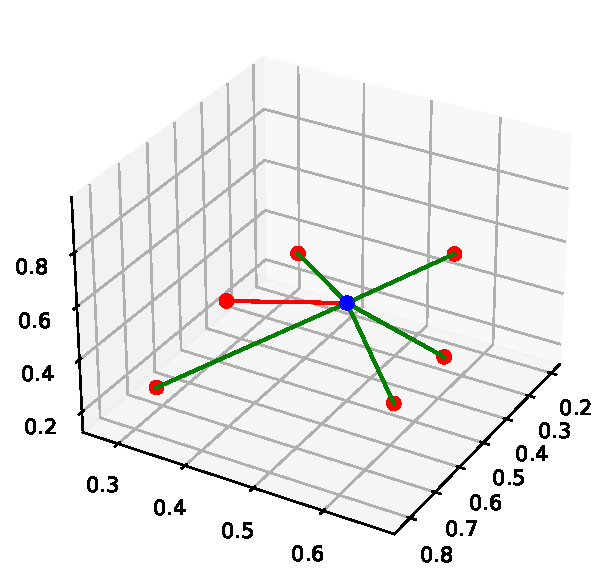
\includegraphics[scale=0.6]{obrazky-figures/hashtree/distance.pdf}
    \caption{Ilustrace vyhledávání nejbližšího souseda z~vybraného uzlu stromu. Modrý bod je vstupním bodem. Červené body jsou body uzlu získaného v~první fázi. Vzdálenosti jsou porovnány a je vybrána ta nejmenší (znázorněna červeně).}
    \label{fig:distance_ilustration}
\end{figure}


\subsection*{K-nejbližší soused}
Vyhledávání $k$-nejbližších sousedů probíhá velmi podobně, jako při hledání prvního souseda. Tentokrát by se hledání dalo rozdělit na tři fáze. První fáze nalezení nejbližšího listového uzlu je stejná jako u~hledání nejbližšího souseda (algoritmus \ref{algo:node_search}). V~druhé fázi je potřeba ve stromu vystoupat od listových uzlů výše do takového uzlu, který obsahuje alespoň $k$ prvků. Následně stačí prvky seřadit podle vzdálenosti k~bodu $p$.

Řazení prvků je realizováno pomocí \emph{std::sort} ze standardní knihovny C++. Této implementaci je dodána funkce pro porovnání prvků, což je vlastně jen operátor větší než, který porovná vzdálenost k~bodu $p$ od dvou vstupních hodnot. Není tedy porovnána hodnota bodů, ale jejich vzdálenost od bodu $p$. Ilustrace je na obrázku \ref{fig:distance_operator_ilustration}.

Po seřazení je navrácen seznam bodů. Implementace ignoruje, zda se v~uzlu nachází více, než požadované množství bodů a vrátí seznam všech, které nalezl ve vybraném uzlu.

\begin{figure}
    \centering
    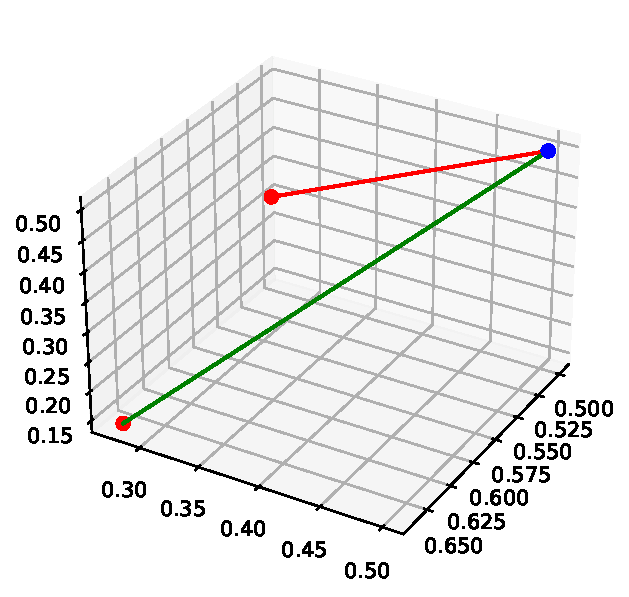
\includegraphics[scale=0.6]{obrazky-figures/hashtree/distance_operator.pdf}
    \caption{Ilustrace operátoru porovnání vzdálenosti k~bod $p$ (znázorněného modře), a dvou porovnávaných bodů (znázorněno červeně) a jejich vzdáleností (červená a zelená). 
    } 
    \label{fig:distance_operator_ilustration}
\end{figure}





\subsection*{Nejbližší soused orientovaný zadaným směrem}
Pro maximální výkon se předpokládají následující možnosti použití:
\begin{enumerate}
    \item První splňující zadaná kriteria.
    \item Nejbližší s~nejpodobnější normálou.
    % \item Iterátor vracejí postupně ty nejvíc podobné body až po ty méně podobné. 
    \item Iterátor se zadanou maximální vzdáleností a vracející postupně ty nejvíc podobné body až po ty méně podobné.
\end{enumerate}

Všechny tyto přístupy budou mít na vstupu jeden bod s~normálou. Podle potřeby mohou obsahovat tyto další parametry:
\begin{itemize}
    \item Míra snažení

    % tady to je chujovo.
    
    Zadává metodě míru snahy, kterou má při vyhledávání projevit. Tímto parametrem se dá nastavit zda-li má vyhledávání probíhat pouze v~listovém uzlu (nastavení $0$), nebo v~úrovni o~jedno větší jak listové případně o~dvě a tak dále.
    \item Tolerance
    
    Jedná se o~číslo na intervalu od $-1$ do $1$. Určuje o~jak moc se může lišit normála bodu. Jedná se o~cosinus úhlu udávající rozdíl normál. 
    \item Maximální vzdálenost
    
    Udává maximální vzdálenost pro vyhledávání.
\end{itemize}

\subsubsection{První splňující zadaná kriteria}
Implementace tohoto vyhledávání je nejjednodušší, ale zároveň by mělo být nejrychlejší. Předpokládá se však značná nepřesnost. Začátek vyhledávání bude jako u~všech popsaných hledání vyhledáním listového uzlu v~hašovací tabulce. Poté budou všechny tyto prvky seřazeny podle vzdálenosti k~zadanému bodu. Takto seřazené pole je potřeba projít prvek po prvku a v~okamžiku, kdy první bod splňuje kriterium, tak je navrácen jako správné řešení. V~případě, že žádný z~prvků nedosahuje kvalit požadovaných vstupem, je vrácena ta nejlepší možnost. Celý postup jde vidět v~algoritmu \ref{algo:firt_knn_normal}.

Tato varianta potřebuje na vstupu parametr zadávající maximální chybu a případně volitelný parametr udávající očekávanou snahu.

Algoritmus využívá metodu popsanou v algoritmu~\ref{algo:node_search}, pojmenovanou jako \empty{find\_node}. Dále pak existuje metoda \emph{tree\_climbing}, která postoupí o~zadaný počet úrovni výše ve stromu a vrátí tento uzel. Funkce \emph{sort} řadí prvky podle vzdálenosti k~bodu $p$. Funkce \emph{dotN} počítá skalární součin normál dvou bodů.

\begin{algorithm}
    \SetAlgoLined
    \KwIn{Vstupní bod $p$, $effort$, $tollerance$}
    \KwOut{Aproximace bodu s~nejpodobnější normálou}

    node = find\_node(p)\;
    
    node = tree\_climbing(node, effort) \;

    sort(node.points, p)



    $Lsimilarity = -1,  Lpoint = \emptyset$ \;
    
    \For{$u \in node.points$} {
        similarity = dotN(u,p)
        
        \If{Lsimilarity < similarity}{
        \If{similarity >= (1 - tollerance)}{
            \Return{u}
        }
        $Lsimilarity = similarity$ \;
        
        $Lpoint = u$ \;
        }

    }
    \Return {Lpoint}
    
    \caption{Algoritmus pro nalezení prvního bodu splňující zadané kriteria.}
    \label{algo:firt_knn_normal}
\end{algorithm}

\subsubsection{Nejbližší soused s~nejpodobnější normálou}
Tento způsob vyhledávání je velmi podobný jako ten předešlý. Rozdíl je v~tom, že vždy projde všechny prvky v~zadaném uzlu a najde tu nejlepší možnost. Celý postup je znázorněn v~algoritmu \ref{algo:knn_normal_leaf}.

\begin{algorithm}
    \SetAlgoLined
    \KwIn{Vstupní bod $p$, $effort$, }
    \KwOut{Aproximovaný bod s~nejpodobnější normálou}

    node = find\_node(p)\;
    
    node = tree\_climbing(node, effort) \;

    sort(node.points, p)



    $Lsimilarity = -1,  Lpoint = \emptyset$ \;
    
    \For{$u \in node.points$} {
        similarity = dotN(u,p)
        
        \If{Lsimilarity < similarity}{
        $Lsimilarity = similarity$ \;
        
        $Lpoint = u$ \;
        }

    }
    \Return {Lpoint}
    
    \caption{Algoritmus pro nalezení nejbližší bodu s~nejpodobnější normálou.}
    \label{algo:knn_normal_leaf}
\end{algorithm}

\subsubsection{Iterátor se zadanou maximální vzdáleností}
V~tomto případě je vyhledávání zahájeno metodou, která vytvoří nový objekt speciálního typu. Tento objekt obsahuje informace potřebné k~vyhledávání podle normály: potencionálně zajímavé body, bod, ke kterému jsou vyhledáváni sousedé a maximální vzdálenost od bodu. Bod a maximální vzdálenost jsou brány z~uživatelského vstupu.

Vyhledávání začíná nalezením listového uzlu. Následně je potřeba procházet strom od listů ke kořenu, dokud nebudou vyfiltrovány všechny body v~požadované vzdálenosti. Tento proces je však aproximován. Aproximace využívá toho, že prostor je rozdělen na krychle o~jednoduše vypočitatelné velikosti z~octree. Velikost se odvíjí od celkové velikosti prostoru $S$ a úrovně zanoření. Pokud je jako listový uzel určen uzel na úrovni $l$, celý prostor je rozdělen celkem na $8^l$ kostek. Hrana každé kostky je rozdělena na $2^l$ dílů. Pokud požadovaná vzdálenost je $D$, pak $\frac{S}{2^l}$ udává počet dílků, který je potřeba. Z~toho plyne, že úroveň lze získat jako $\log_2\left(\frac{S}{D}\right)$, což informuje o~tom, jak vysoko je potřeba vystoupat.

Tento postup nevyžaduje iterování skrz body. Do struktury jsou nahrány body a již zmíněné údaje.

Poté je možné nad vytvořeným objektem volat metodu \emph{next}, která s~každým zavoláním vrátí další bod s~nejpodobnější normálou. Pokud zbývá už jen jeden bod, vrací pořád dokola tentýž. O~prázdnosti iterátoru se lze dotázat metodou \emph{isEmpty}.


\section{Testování přesnosti}
\label{presnost}

Při testování přesnosti bylo pomocí kontrolní implementace vygenerováno 50 různých množin náhodných bodů o~mohutnosti $100$ až $10^6$. Celkem tedy 250 různých množin bodů, dále pak bylo vygenerováno 1000 náhodných bodů jako vstupy pro algoritmus nejbližšího souseda. Kontrolní implementace seřadí tyto body podle vzdálenosti k~vstupnímu bodu. Poté je spuštěna testovaná implementace a porovnají se výsledky.

\subsection*{Nejbližší soused}
Implementovaná struktura není 100 procentně přesná, jak je možné vidět na grafech \ref{fig:accurucybench}, tak je přesná a nepřesnost  nikdy nepřekročila 5 procent. Z~naměřených výsledků lze vyčíst, že kriterium $M_{max}$ má minimální vliv na přesnost. Daleko větší vliv má mohutnost vstupní množiny bodů, což jde vidět na grafu \ref{fig:accurucybench_err_points}.

Na grafu \ref{fig:accurucybench_err_mmax} jde vidět, jak s~rostoucím počtem bodů roste přesnost, která se u~větších sad bodů blíží ke 100 procentům. Určitě bude platit, že s~rostoucím počtem $M_{max}$ bude růst přesnost, neboť je strom čím dál tím méně hluboký a výpočet se přibližuje výpočtu hrubou silou. 


\begin{figure}
 
\begin{subfigure}[t]{0.49\columnwidth}
    \centering  
    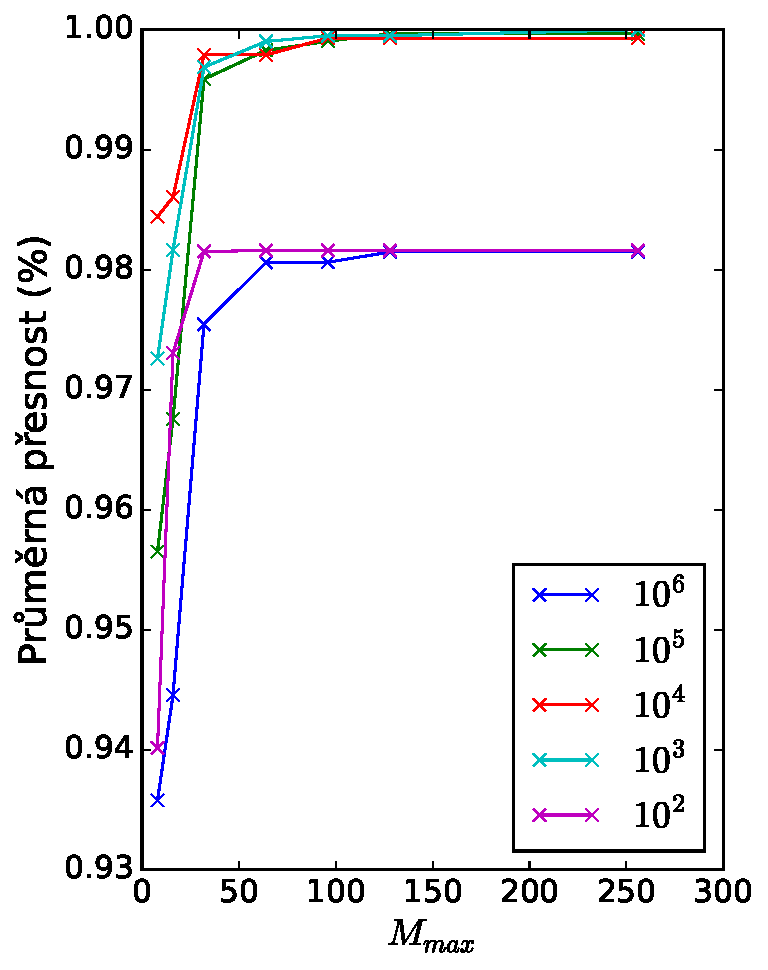
\includegraphics[scale=0.6]{obrazky-figures/benchmark/accuracy/benchmark_accuracy_by_mmax.pdf}
    \caption{Porovnání průměrné úspěšnosti nalezení nejbližšího správného souseda vzhledem ke kriteriu $M_{max}$.}
\label{fig:accurucybench_acc_mmax}
\end{subfigure}
\hfill
\begin{subfigure}[t]{0.49\columnwidth}
    \centering  
    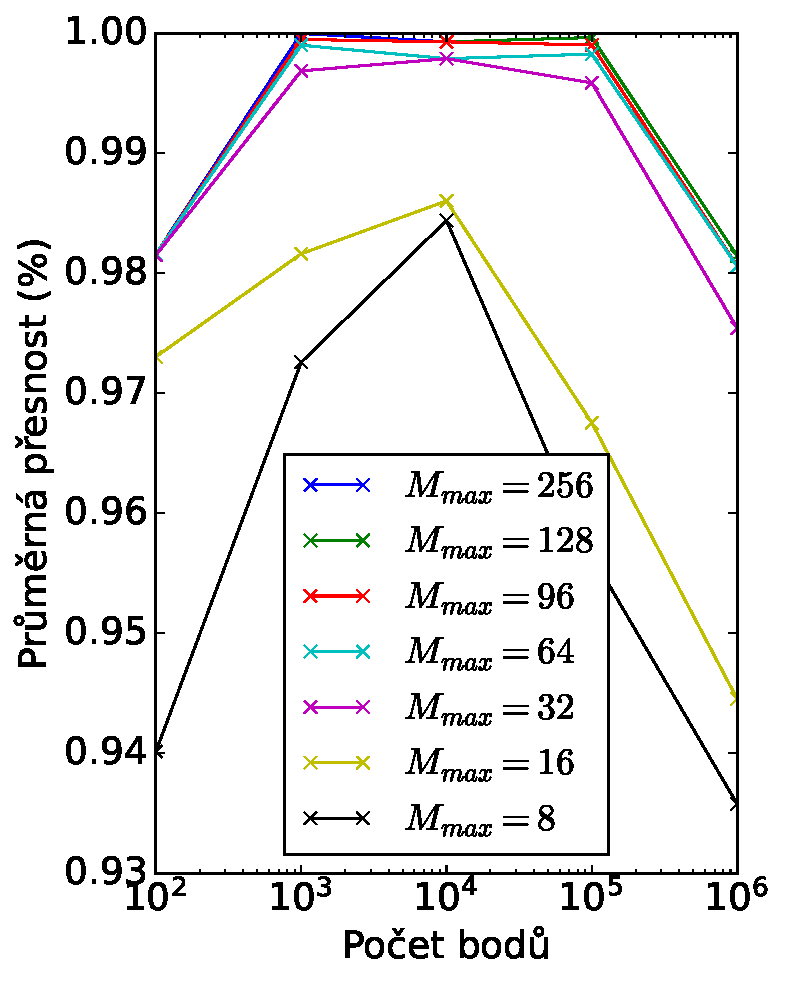
\includegraphics[scale=0.6]{obrazky-figures/benchmark/accuracy/benchmark_accuracy_by_points.pdf}
    \caption{Porovnání průměrné úspěšnosti nalezení nejbližšího správného souseda vzhledem k~počtu bodů.}
    \label{fig:accurucybench_acc_points}
\end{subfigure}
\hfill
\begin{subfigure}[t]{0.49\columnwidth}
    \centering  
    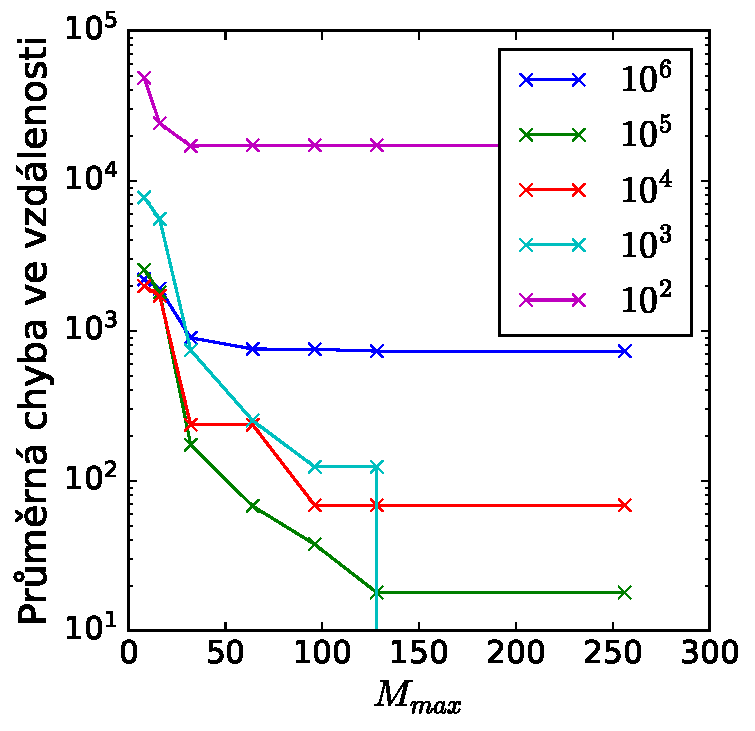
\includegraphics[scale=0.6]{obrazky-figures/benchmark/accuracy/benchmark_avgerr_by_mmax.pdf}
    \caption{Porovnání průměrné úspěšnosti nalezení nejbližšího správného souseda vzhledem ke kriteriu $M_{max}$.}
    \label{fig:accurucybench_err_mmax}


\end{subfigure}
\hfill
\begin{subfigure}[t]{0.49\columnwidth}
    \centering  
    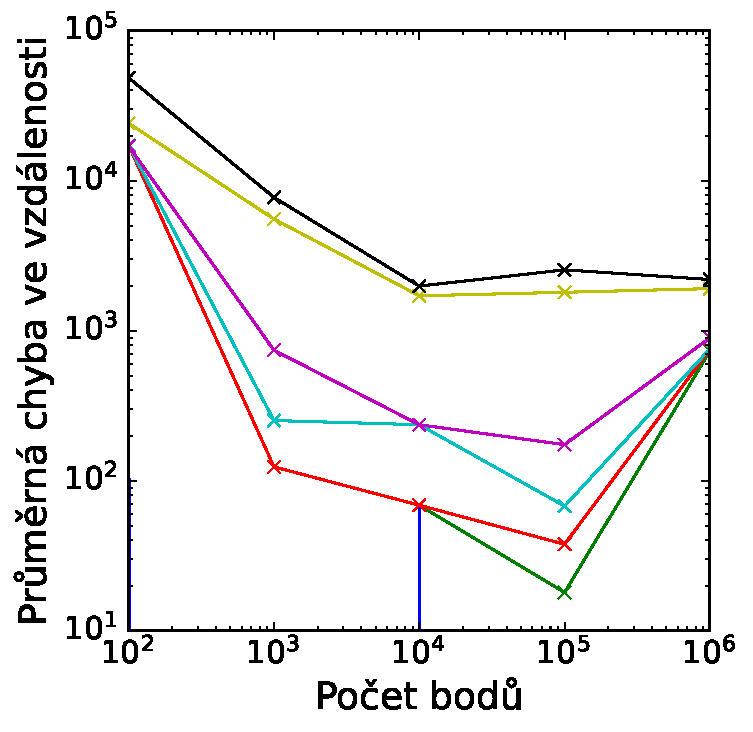
\includegraphics[scale=0.6]{obrazky-figures/benchmark/accuracy/benchmark_avgerr_by_points.pdf}
    \caption{Porovnání průměrné odchylky vzdálenosti od správného nejbližšího souseda vzhledem k~počtu bodů\footnote{Legenda pro tento graf se nachází na na \ref{fig:accurucybench_acc_points}}.}
\label{fig:accurucybench_err_points}

\end{subfigure}



\caption{Grafy ukazující přesnost pro náhodné body na intervalu $-(10^6)$ až $10^6$ }
\label{fig:accurucybench}
\end{figure}



\subsection*{K-nejbližší soused}
Testování probíhalo výše popsaným způsobem pro body na intervalu $-(10^6)$ až $10^6$. Po algoritmu bylo požadováno, aby navracel nejbližší sousedy pro $k \in \{8,16,32,64,128,256,512, \\ 1000\}$. Všechny tyto množiny byly vyhledávány ve stromech s~$M_{max} \in \{8,16,32,64,96,128,256\}$. Hodnoty byly zvoleny tak, aby každý strom vybudovaný s~jakýmkoliv parametrem byl nucen vyhledávat i jinde než v~listovém uzlu.

Jako přesnost je uváděna hodnota, kde je podělen celkový počet možnosti k~výskytu chyby (tzn. například u~$k=16$ to je 16) a uskutečněných chyb. Například pokud by v~seznamu 16 prvků bylo 8 špatně, tak by přesnost byla stanovena jako 0.5.

Z~grafů \ref{fig:knn_accuracy} je patrné, že přesnost značně klesá s~počtem bodů. Nicméně průměrná chyba paradoxně klesá. Struktura tedy s~přibývajícím počtem bodů nedává absolutně nejbližší prvky, ale vypočítává přibližně správné sousedy.

\begin{figure}
 
\begin{subfigure}[t]{.5\columnwidth}
    \centering  
    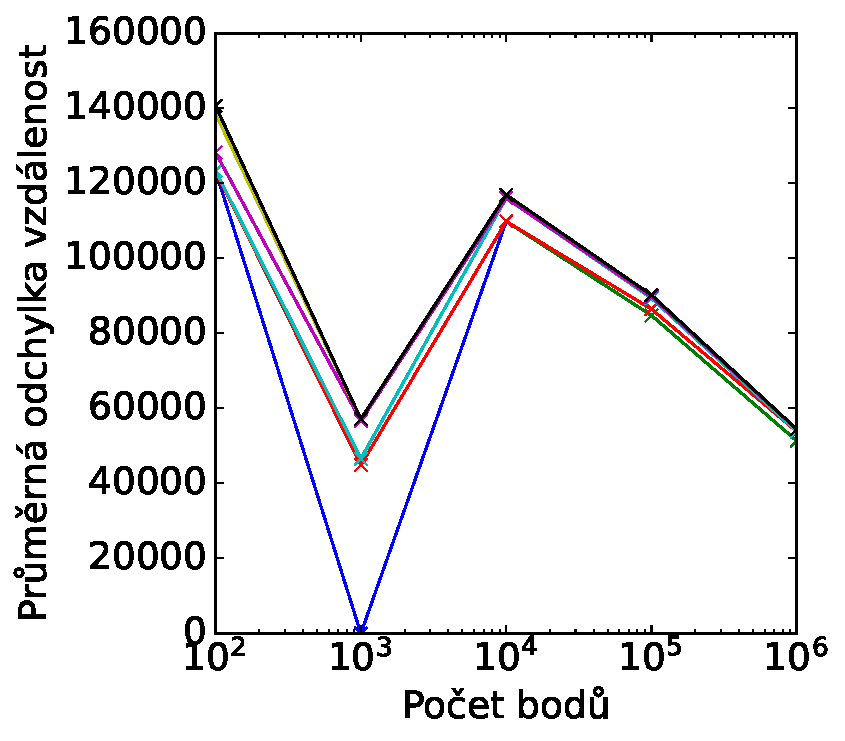
\includegraphics[scale=0.55]{obrazky-figures/benchmark/knn/benchmark_knn_acc_err.pdf}

\end{subfigure}
\hfill
\begin{subfigure}[t]{.5\columnwidth}
    \centering  
    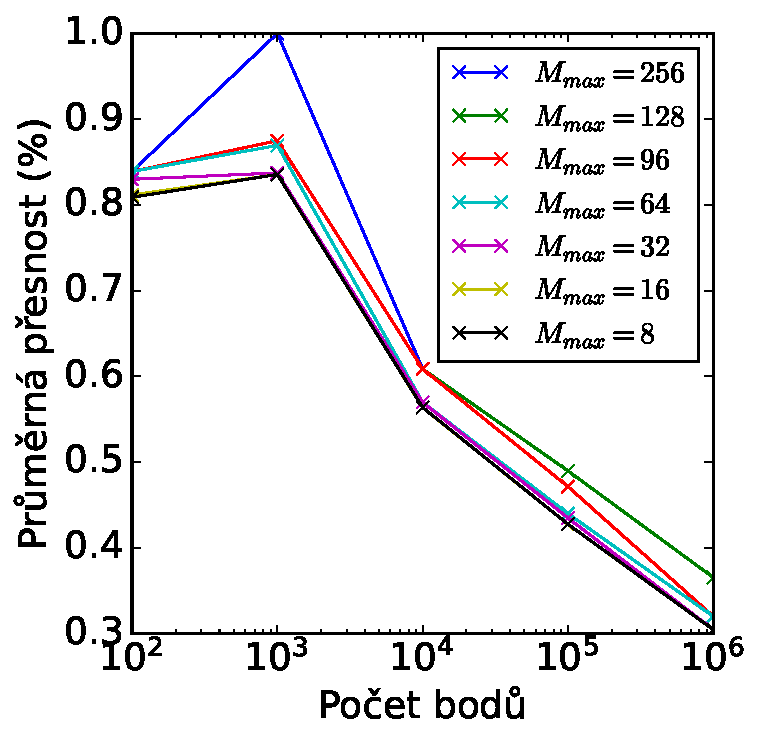
\includegraphics[scale=0.55]{obrazky-figures/benchmark/knn/benchmark_knn_acc.pdf}

\end{subfigure}
    \caption{Přesnost algoritmu k-NN nad náhodnými body na intervalu $-(10^6)$ až $10^6$. }
\label{fig:knn_accuracy}


\end{figure}

\subsection*{Nejbližší soused orientovaný zadaným směrem}
Pro testování této funkcionality byly použity jiné množiny než u~testování předešlých dvou funkcionalit. Na obrázcích \ref{fig:nn-fig-normal-examples} jsou zobrazeny množiny bodů, které budou testovány. Kompletní plocha, ze které byly body spočteny se nachází na obrázku \ref{fig:nn-fig-normal-examples-plane}. Tato plocha je vlastně normální rozdělení pro 2D prostor. 

Mimo souřadnice je potřeba vygenerovat i normály. Normály jsou generovány jako směrový vektor ke středu normálního rozdělení. Tyto vektory jsou normalizovány. 

\subsubsection{Kontrolní implementace}
Kontrolní implementace pracuje se dvěma množinami bodů. První množinou je množina $P$. Tato množina je určená vstupem a vyhledávají se v ní sousedé. Druhou množinou je množina $T$, obsahující množiny množin bodů. Každá z těchto množina reprezentuje vstupy pro test. Aby byly testy směrodatné, bylo vygenerováno 30 takových množin. Tyto množiny obsahují body, které rovněž leží na této ploše, každá s~počtem 100 bodů. Pro účely testování přesnosti se tedy uskuteční $3000$ různých vyhledání nad všemi vstupními množinami. Všechny tyto body jsou na intervalu -($10^6$) až $10^6$. 

Implementace shromažďuje všechny body se vzdáleností menší jak sto tisíc. Potom jsou tyto body seřazeny podle normály a 10 nejlepších je uloženo pro porovnání. 

\subsubsection{Přesnost}
Přesností u~algoritmů vracející pouze jeden bod (hrubé aproximace) je myšleno procento případů, které vrátily stejný bod jako kontrolní implementace. Pokud nevrátily stejný bod, tak implementace počítá průměrnou odchylku normály a vzdálenosti. Pokud jde o~přesnost u~implementace s~iterátorem, rozumí se tím kolik z~10 bodů vrátil iterátor správně včetně pořadí. 

Na obrazcích \ref{fig:accurucybench_normal_acc} jde vidět, že u~hrubých aproximací klesá přesnost s~rostoucím počtem bodů. Stejně, tak to je i s~chybou, která roste, ale postupně se růst zpomaluje. Iterátor nevrací exaktně přesné sousedy. Vzhledem k tomu, jak aproximuje iterátor vzdálenost nedává příliš smysl měřit exaktní přesnost. Mnohem lepší představu o kvalitě výsledků lze vyčíst z průměru odchylek vzdáleností a normály. Vývoj těchto údajů si lze prohlédnout na obrázku \ref{fig:accurucybench_normal_distance} a \ref{fig:accurucybench_normal_normal}. Při pohledu na obrázek \ref{fig:accurucybench_normal_distance}, lze vidět, že chyby ve vzdálenosti s rostoucí množinou vstupních bodů sice rostou, ale růst se postupně zpomaluje. 

Přesnost u~podobnosti normály je velmi dobrá u~všech algoritmů. U~malých množin je nepřesnost větší kvůli aproximacím týkající se vzdáleností. Vývoj přesností u~všech hrubých akceleracích je stejný, jak ukazuje graf \ref{fig:accurucybench_normal_normal}. U~poslední implementace se přesnost normály blíží ke sto procentům už u~malých množin.

Z~výsledků je patrné, že největší problém pro tyto aproximace je správné určení zkoumaných bodů pro vyhledání podobné orientace. I~přesto však všechny implementace přinášejí výsledky, které jsou uvažovatelné pro nasazení u~některých aplikací. Kriterium $M_{max}$, tentokrát významně neovlivňuje téměř nic. Z~testů je taky patrné, že nastavit \emph{effort} na hodnotu 1, minimálně na testovaných datech nemá žádný smysl z~pohledu přesnosti. 



\begin{figure}
 
\begin{subfigure}[t]{0.49\columnwidth}
    \centering  
    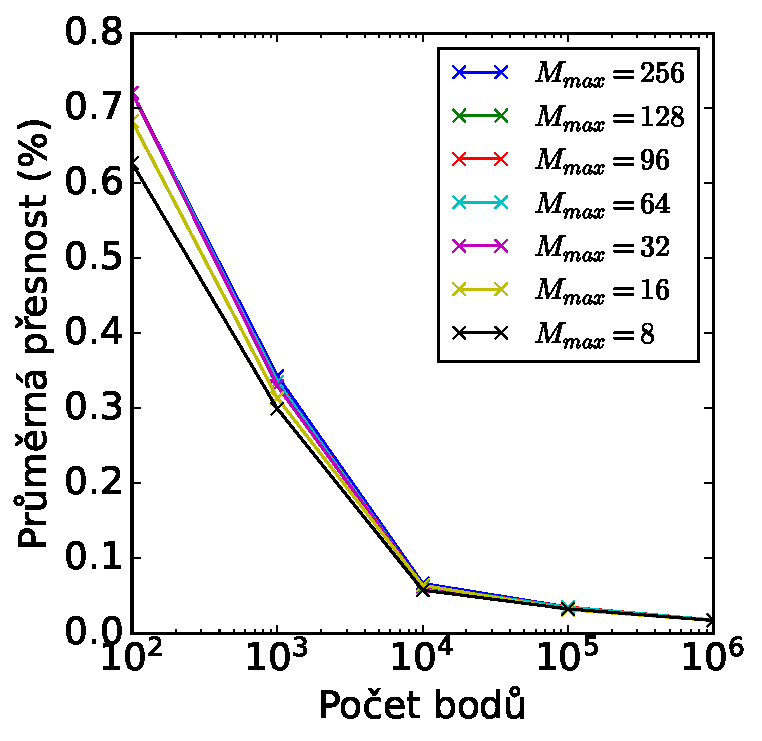
\includegraphics[scale=0.6]{obrazky-figures/benchmark/accuracy/normal/acccurucy_first_err_cases.pdf}
    \caption{Přesnost algoritmu \uv{První splňujícími zadané kriteria}.}

\end{subfigure}
\hfill
\begin{subfigure}[t]{0.49\columnwidth}
    \centering  
    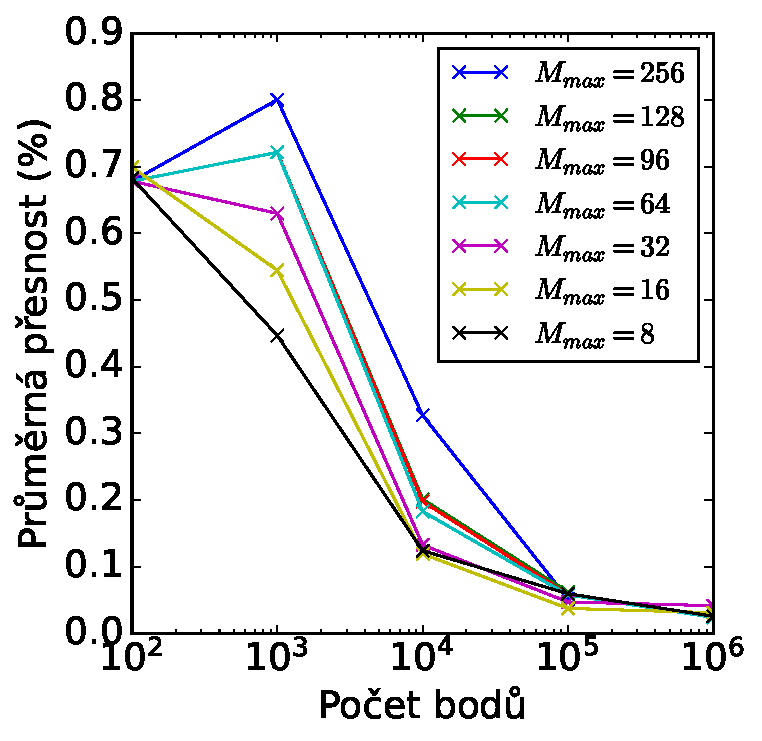
\includegraphics[scale=0.6]{obrazky-figures/benchmark/accuracy/normal/acccurucy_leaf_err_cases.pdf}
    \caption{Přesnost algoritmu \uv{Nejbližší s~nejpodobnější normálou}.}

\end{subfigure}
\hfill
\begin{subfigure}[t]{0.49\columnwidth}
    \centering  
    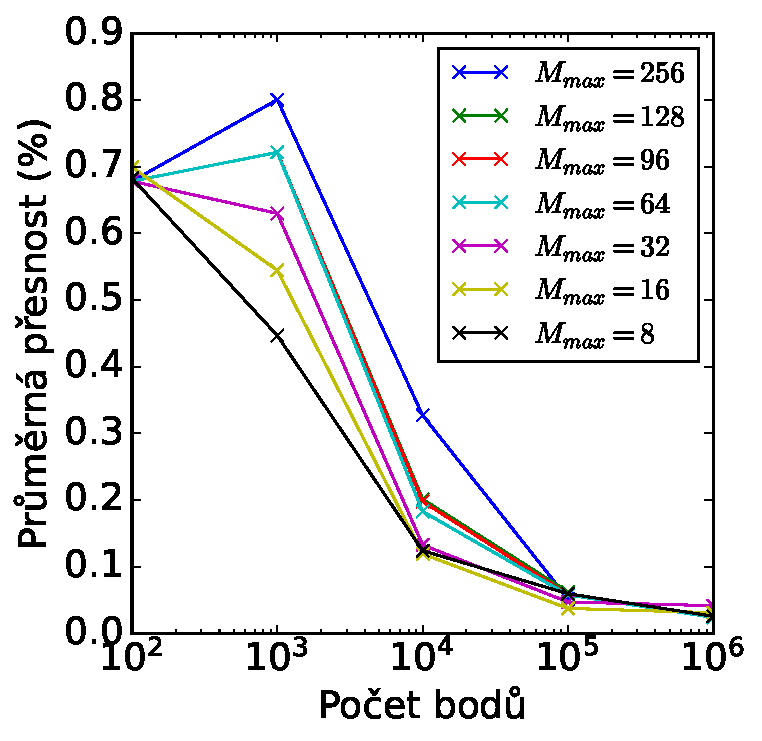
\includegraphics[scale=0.6]{obrazky-figures/benchmark/accuracy/normal/acccurucy_leaf1_err_cases.pdf}
    \caption{Přesnost algoritmu \uv{Nejbližší s~nejpodobnější normálou} s~nastaveným parametrem \emph{effort} na $1$.}
\end{subfigure}
\hfill
\begin{subfigure}[t]{0.49\columnwidth}
    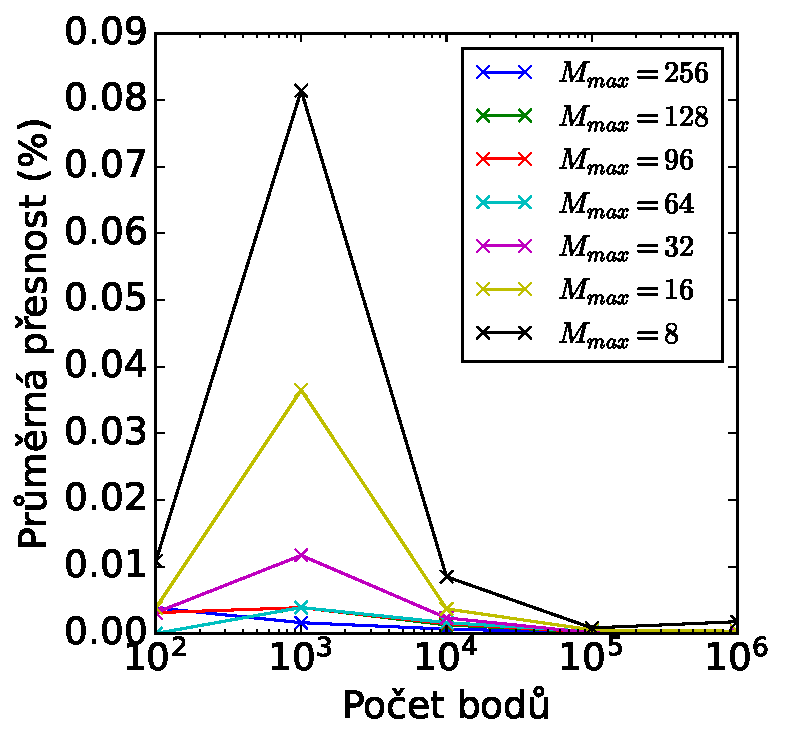
\includegraphics[scale=0.6]{obrazky-figures/benchmark/accuracy/normal/acccurucy_it_err_cases.pdf}
    \centering  
    \caption{Přesnost vypočtu pomocí iterátoru s~aproximací vzdálenosti. Přesnost v~úspěšnosti uhodnuti deseti nejpodobnějších bodů. }

\end{subfigure}
\caption{Přesnost ve výpočtech nejbližších sousedů s~nejpodobnější normálou.}
\label{fig:accurucybench_normal_acc}

\end{figure}


\begin{figure}
 
\begin{subfigure}[t]{0.49\columnwidth}
    \centering  
    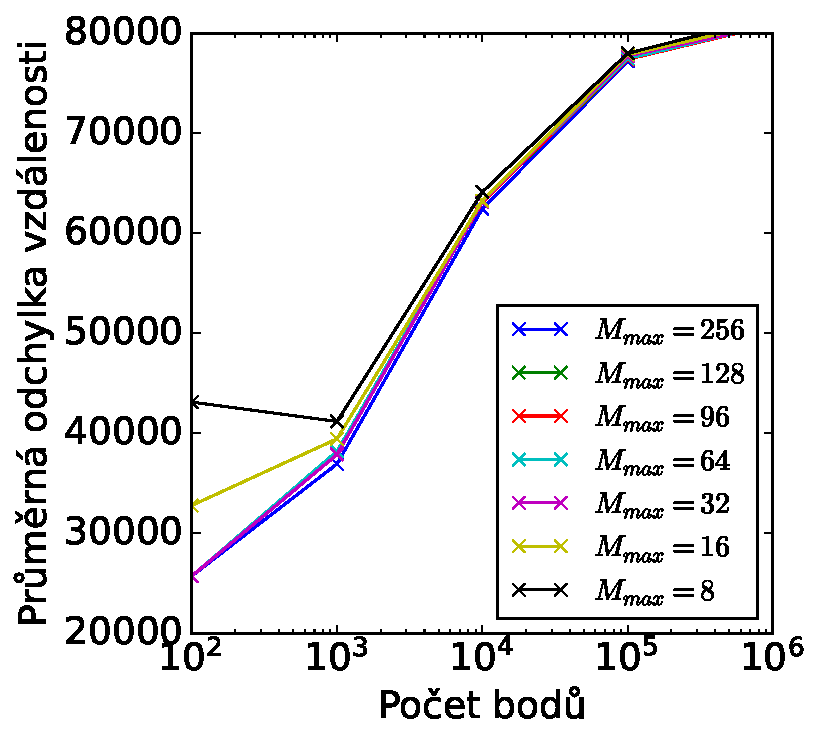
\includegraphics[scale=0.6]{obrazky-figures/benchmark/accuracy/normal/acccurucy_first_err_distance.pdf}
    \caption{Odchylka vzdálenosti při výpočtu pomocí \uv{První splňujícími zadané kriteria v~uzlu}.}

\end{subfigure}
\hfill
\begin{subfigure}[t]{0.49\columnwidth}
    \centering  
    \includegraphics[scale=0.6]{obrazky-figures/benchmark/accuracy/normal/acccurucy_leaf_err_distance.pdf}
    \caption{Odchylka vzdálenosti při výpočtu pomocí \uv{Nejbližší s~nejpodobnější normálou}.}

\end{subfigure}
\hfill
\begin{subfigure}[t]{0.49\columnwidth}
    \centering  
    \includegraphics[scale=0.6]{obrazky-figures/benchmark/accuracy/normal/acccurucy_leaf1_err_distance.pdf}
    \caption{Odchylka vzdálenosti při výpočtu pomocí  algoritmu \uv{Nejbližší s~nejpodobnější normálou} s~nastaveným parametrem \emph{effort} na $1$.}
\end{subfigure}
\hfill
\begin{subfigure}[t]{0.49\columnwidth}
    \includegraphics[scale=0.6]{obrazky-figures/benchmark/accuracy/normal/acccurucy_it_err_distance.pdf}
    \centering  
    \caption{Odchylka vzdálenosti při výpočtu pomocí iterátoru s~aproximací vzdálenosti. Přesnost v~úspěšnosti uhodnuti deseti nejpodobnějších bodů. }

\end{subfigure}
\caption{Chyby vzdálenosti ve výpočtech nejbližších sousedů s~nejpodobnější normálou.}
\label{fig:accurucybench_normal_distance}

\end{figure}


\begin{figure}
 
\begin{subfigure}[t]{0.49\columnwidth}
    \centering  
    \includegraphics[scale=0.6]{obrazky-figures/benchmark/accuracy/normal/acccurucy_first_err_normal.pdf}
    \caption{Odchylka normály při výpočtu pomocí \uv{První splňujícími zadané kriteria v~uzlu}.}

\end{subfigure}
\hfill
\begin{subfigure}[t]{0.49\columnwidth}
    \centering  
    \includegraphics[scale=0.6]{obrazky-figures/benchmark/accuracy/normal/acccurucy_leaf_err_normal.pdf}
    \caption{Odchylka normály při výpočtu pomocí \uv{Nejbližší s~nejpodobnější normálou}.}

\end{subfigure}
\hfill
\begin{subfigure}[t]{0.49\columnwidth}
    \centering  
    \includegraphics[scale=0.6]{obrazky-figures/benchmark/accuracy/normal/acccurucy_leaf1_err_normal.pdf}
    \caption{Odchylka normály při výpočtu pomocí  algoritmu \uv{Nejbližší s~nejpodobnější normálou} s~nastaveným parametrem \emph{effort} na $1$.}
\end{subfigure}
\hfill
\begin{subfigure}[t]{0.49\columnwidth}
    \includegraphics[scale=0.6]{obrazky-figures/benchmark/accuracy/normal/acccurucy_it_err_normal.pdf}
    \centering  
    \caption{Odchylka normály při výpočtu pomocí iterátoru s~aproximací vzdálenosti.}

\end{subfigure}
\caption{Chyby v~normále ve výpočtech nejbližších sousedů s~nejpodobnější normálou.}
\label{fig:accurucybench_normal_normal}

\end{figure}



\begin{figure}
   \centering
\begin{subfigure}[t]{0.45\columnwidth}
    \centering
    \includegraphics[scale=0.5]{obrazky-figures/knn_norm/points_3d normal_plane_100.pdf}
    \caption{$10^2$ bodů}
\end{subfigure}
\hfill
\begin{subfigure}[t]{0.45\columnwidth}
    \centering
    \includegraphics[scale=0.5]{obrazky-figures/knn_norm/points_3d normal_plane_1000.pdf}
    \caption{$10^3$ bodů}
\end{subfigure}
\hfill
\begin{subfigure}[t]{0.45\columnwidth}
    \centering
    \includegraphics[scale=0.5]{obrazky-figures/knn_norm/points_3d normal_plane_10000.png}
    \caption{$10^4$ bodů}
    \end{subfigure}
\hfill
\begin{subfigure}[t]{0.45\columnwidth}
\centering
\includegraphics[scale=0.45]{obrazky-figures/knn_norm/points_3d normal_plane_100000.png}
    \caption{$10^6$ bodů}
\end{subfigure}
\hfill

    \caption{Grafické znázornění rozložení bodů, na kterých byl testován algoritmus nejbližšího souseda s~porovnáním normály. Množství bodu na obrázcích je od $10^2$ až $10^6$. }
    \label{fig:nn-fig-normal-examples}
\end{figure}

\begin{figure}

\begin{subfigure}[t]{0.5\columnwidth}
\centering
\includegraphics[scale=0.47]{obrazky-figures/knn_norm/points_3d normal_plane_continuouse.pdf}
    \caption{Grafické znázornění plochy jenž byla použita pro generování bodů pro testování algoritmu nejbližšího souseda a s~porovnáním normály. }
        \label{fig:nn-fig-normal-examples-plane}
\end{subfigure}
\hfill
\begin{subfigure}[t]{0.5\columnwidth}
\centering
\includegraphics[scale=0.49]{obrazky-figures/knn_norm/points_2d_normals_ilustration.pdf}
    \caption{Grafické ilustrace průřezu plochy a bodů procházející, spolu s~jejich normálou směřující k~bodu (0,0).}
\end{subfigure}

\end{figure}

\subsubsection{}



\section{Testování výkonu a paměťové náročnosti}
\label{vykon}


Testování probíhalo na procesoru \emph{AMD Ryzen 9 7950X3D} s~32 vlákny, spolu s~64\,GB paměti RAM. Jako operační systém bylo použito \emph{Ubuntu 22.04.4 LTS} s~\emph{5.15.0-102-generic} verzí kernelu. Pro překlad bylo použito \emph{gcc 13.1.0} (Ubuntu 13.1.0-8ubuntu1\textasciitilde{}22.04). Překlad probíhal s~překladovými flagy:

\begin{itemize}
    \item \texttt{-Ofast -DNDEBUG -std=c++20 -march=native -fpic -ftree-vectorize \\ 
    -ffast-math -flto -o3},
\end{itemize}
pokud není uvedeno jinak. Každý test byl spuštěn padesátkrát a všechny uváděné hodnoty jsou průměry z~50 běhů. Implementace měla k~dispozici všech 32 vláken procesoru. Pro výkonnostní benchmarky byl použit framework \emph{Google Benchmark}\footnote{\url{https://github.com/google/benchmark}}.


Pseudonáhodné body byly generovány pomocí \emph{default\_random\_engine} ze standardní knihovny C++.

\subsection*{Výstavba struktury}
Struktura se staví umístěním všech bodů najednou a není vhodné v~průběhu přidávat další body, neboť to vyžaduje kompletní přepočítání. Předpokládá se užití struktury v~režimu, kdy je předem počítána a následně používána v~komplexnějším nasazení, kde se s~ní bude intenzivně pracovat po dlouhou dobu.


\subsubsection{Vliv kriteria $M_{max}$ na výstavbu stromu}

Jak je možné vidět na grafech \ref{fig:benchmark_builtime_points_Mmax}, $M_{max}$ je velmi znatelný parametr, který ovlivňuje čas potřebný k~výstavbě struktury. Na grafu lze vidět, jak pro malé množiny trvá budování stromu téměř stejný čas, ale s~rostoucí množinou se ukazuje, kdy je vhodné zvolit jaké kriterium $M_{max}$. Například u~velikosti $10^6$ je nejrychlejší výstavba stromu pro kriterium $M_{max}=128$. Jak je vidět na obrázcích \ref{fig:benchmark_builtime_points_Mmax_25} a \ref{fig:benchmark_builtime_points_Mmax_5}, růst má velmi rozdílnou charakteristiku pro různě velké vstupní množiny.

\begin{figure}
 
\begin{subfigure}[t]{0.29\columnwidth}
    \centering  
    \includegraphics[scale=0.4]{obrazky-figures/benchmark/benchmark_builtime_points_Mmax.pdf}

    \caption{Růst časové složitosti vzhledem k~počtu bodů pro zvolená kriteria $M_{max}$. }
            \label{fig:benchmark_builtime_points_Mmax_all}
\end{subfigure}
\hfill
\begin{subfigure}[t]{0.29\columnwidth}
    \centering  
    \includegraphics[scale=0.4]{obrazky-figures/benchmark/benchmark_builtime_points_lowest.pdf}

    \caption{Růst časové složitosti vzhledem k~počtu bodů pro vstupní počet bodů $10^3$.}
        \label{fig:benchmark_builtime_points_Mmax_25}
\end{subfigure}
\hfill
\begin{subfigure}[t]{0.29\columnwidth}
    \centering  
    \includegraphics[scale=0.4]{obrazky-figures/benchmark/benchmark_builtime_points_highest.pdf}

    \caption{Růst časové složitosti vzhledem k~počtu bodů pro vstupní počet bodů $10^6$. }
        \label{fig:benchmark_builtime_points_Mmax_5}
    
\end{subfigure}
\hfill
\begin{subfigure}[t]{1\columnwidth}
    \includegraphics[scale=0.4]{obrazky-figures/benchmark/benchmark_builtime_points_Mmax_bar.pdf}

    \caption{Růst časové složitosti vzhledem k~počtu bodů pro kriterium $M_{max}=5$. }
        \label{fig:benchmark_builtime_points_Mmax_bar}
\end{subfigure}

    \caption{Grafy zachycující závislost mezi počtem bodů $M_{max}$ a dobou výstavby struktury.}
    \label{fig:benchmark_builtime_points_Mmax}

\end{figure}


Růst počtu uzlů je možné vidět na grafu \ref{fig:benchmark_nodes_points_Mmax}. Je potřeba si uvědomit, že mimo samotného stromu je potřeba mít v~paměti i hašovací tabulku, jenž obsahuje všechny uzly stromu, čímž roste celkové využití paměti o~to rychleji. Na grafu jde vidět, že používat nízká kriteria $M_{max}$ se pro větší množství bodů absolutně nevyplatí. Na druhou stranu u~k-nejbližšího souseda zase algoritmus benefitu-je z~nižšího $M_{max}$, ale u~nejbližšího souseda to vyhledávání spíš zpomaluje.

\begin{figure}

    \begin{subfigure}[t]{1\columnwidth}
        \centering
        \includegraphics[scale=0.4]{obrazky-figures/benchmark/benchmark_median_points_memory.pdf}


    \end{subfigure}
    \caption{Růst počtu uzlů stromu pro náhodné body vzhledem k~počtu bodů pro zvolená kriteria $M_{max}$. }
    \label{fig:benchmark_nodes_points_Mmax}

\end{figure}

\subsection*{Výkonnost algoritmu nejbližšího souseda}
Při optimalizacích vyhledávání nejbližšího souseda se ukázalo, že nejužším hrdlem je implementace hašovací tabulky ze standardní knihovny\footnote{\url{https://www.youtube.com/watch?v=M2fKMP47slQ}}. Při profilování byl zjištěno, že vyhledání prvku v~hašovací tabulce zabírá více, než 70 procent času vyhledávání. Vyhledání nejmenšího prvku je vektorizováno, a proto je vhodné kriterium $M_{max}$ zvolit jako násobky osmi, aby se maximálně využilo potenciálu AVX. 

Vzhledem k~na měřeným datům lze konstatovat, že je vhodné zvolit kriterium $M_{max}$ ze znalostí mohutnosti množiny vstupních bodů. Pak lze dosáhnout nejoptimálnějšího výsledku. Graf \ref{fig:nn_benchmark} ukazuje že, větší $M_{max}$ je vhodný pro větší vstupní množiny. Například si je možné porovnat $M_{max}=32$ u~$10^4$ a $10^5$, kde se začíná projevovat toto zrychlení.  

U~malých vstupních množin se rychlost NN téměř nemění napříč mnoha kriterii $M_{max}$. Především to platí pro $M_{max} \geq 64$. Tento fakt lze vysvětlit tím, že všechny body se vejdou přímo do kořene nebo jen do první úrovně stromu. 

Vyhledávání pro malé množiny je u~této struktury značně neefektivní a pomalé. Zbytečnému binárnímu vyhledávání nad stromem, který má jen velmi malou hloubku a tím pádem i minimální počet uzlů, způsobuje značné zpomalení. Jedná se v~podstatě o~zpomalené vyhledávání hrubou silou. 

Graf \ref{fig:nn_benchmark} ukazuje, pro jak velké vstupní množiny je vhodné zvolit které kriterium $M_{max}$.

Přímé srovnání s~původní implementaci není možné. Autoři nezveřejnili zdrojové kódy a není možné provést benchmarky na stejném stroji. Zdá se však, že tato varianta je  asi 2x až 3x pomalejší, což je velmi pravděpodobně způsobeno nevhodně zvolenou implementací hašovací tabulky. Je potřeba dodat, že obě varianty naleznou nejbližší sousedy během několika málo stovek nanosekund.

\begin{figure}
 
\begin{subfigure}[t]{1\columnwidth}
    \centering  
    \includegraphics[scale=0.45]{obrazky-figures/benchmark/nn/benchmark_nn_points_Mmax.pdf}

\end{subfigure}

\begin{subfigure}[t]{1\columnwidth}
    \centering  
    \includegraphics[scale=0.40]{obrazky-figures/benchmark/nn/benchmark_nnspeed_points_Mmax_bar.pdf}

\end{subfigure}
    \caption{Porovnání rychlosti NN pro různé nastavení $M_{max}$ a různé počty bodů. }
\label{fig:nn_benchmark}



\end{figure}

\subsection*{Výkonnost algoritmu k-nejbližšího souseda}
Obrázek \ref{fig:kn_benchmark} představuje struktura, která byla použita pro vyhledávání $k$-nejbližších sousedů z~hlediska rychlosti. Z~toho vyplývá, že se vyplatí používat co možná nejmenší kriterium $M_{max}$. Zajímavostí může být to, že u~všech testovaných $k$ bylo rychlejší vyhledávat větší $k$ než nastavené kriterium $M_{max}$. Vysvětlením tohoto úkazu je to, že vybudovaný strom obsahuje v~listových uzlech jeden až $M_{max}$ bodů. Pokud vyhledaný listový uzel obsahuje bodů méně, jak požadované množství, tak algoritmus vystoupá do otce, kde může v~nejhorším případě nalézt až osm krát tolik uzlů\footnote{$8 \cdot M_{max} -1$ je největší počet uzlů}. Tento jev vytváří znatelné zpomalení, protože je potřeba seřadit mnohem více prvků než pouze $k$ respektive $M_{max}$. Vyhledávání v~nejlepším případě v~1 milionů bodů trvá  přibližně $1550$ nanosekund.

Výkon je stejně jako u~NN limitována hašovací tabulkou. Znatelný hendikep je inicializace a vkládání hodnot do vektoru, který má být navrácen. Další drahou operací je řazení prvků podle vzdálenosti. Jak řazení tak inicializaci by se dalo vyhnout tak, že by algoritmus vracel odkaz na interní pole bodů nacházející se v~listovém uzlu. V~takovém případě by, ale body nebyly seřazeny a bylo by potřeba se smířit s~chybou.

 \begin{figure}
 \begin{subfigure}[t]{0.5\columnwidth}
    \centering  
    \includegraphics[scale=0.4]{obrazky-figures/benchmark/knn_speed/benchmark_k_mmax_1m.pdf}
\caption{Graf pro vstupní množinu bodů o~mohutnosti $10^6$}
\hfill
\end{subfigure}
\begin{subfigure}[t]{0.5\columnwidth}
    \centering  
    \includegraphics[scale=0.4]{obrazky-figures/benchmark/knn_speed/benchmark_k_mmax_1k.pdf}

\caption{Graf pro vstupní množinu bodů o~mohutnosti $10^3$}
\end{subfigure}

    \caption{Grafy pro velikosti vstupních množin $10^3$ a $10^6$ $k$-NN algoritmu. Podobné charakteristiky mají i ostatní testované mohutnosti bodů. U~$k \in \{256,512,1000\}$ se hodnoty překrývají.  }
\label{fig:kn_benchmark}



\end{figure}

\subsection*{Výkonnost algoritmu nejbližšího souseda s~porovnáním normály}
V obrázcích \ref{fig:nn_normal_benchmark}, si lze povšimnout toho, že varianta pro prohledávání všech bodů náležející do listového uzlů je rychlejší, než ta která vrací první bod splňující kritéria. Ačkoliv při návrhu se počítalo s přesně opačným výsledkem. Vzhledem k tomu, že tato varianta je i přesnější je vhodné použít tuto variantu, pro získání prvního bodu. Nečekaný výsledek je způsoben lepší vektorizací. Pro $M_{max}$ jde vidět, jak je růst složitosti s rostoucí množinou vstupních bodů velmi pozvolný. Je tedy vhodné použít malé $M_{max}$, ale je potřeba počítat s vysokou paměťovou náročností. 

Další věc, které si lze všimnou z grafů, se týká implementace vracející první vyhovující bod. Jde vidět, jak s rostoucím počtem bodů se potenciálně vyhovující bod může nacházet až na konci pole, což způsobuje čím dál tím markantnější zpomalení.

Pro iteratorovou implementací není rychlost vyhledání jediný sledovaný parametr. Je potřeba i přihlédnout k době, za kterou se vystaví tato iterační struktura, znázorněna na grafu \ref{fig:nn_normal_benchmark_it}. Tento čas je velmi variabilní. Záleží totiž na, jak vysoko je potřeba vystoupat ve stromu a taky na $M_{max}$. Pro rychlost je vhodné zvolit kriterium $M_{max}$, kvůli přesnějším aproximacím vzdáleností a taky kvůli menší mohutnosti stromových uzlů, způsobené větší hloubkou stromu. 
\begin{figure}[ht]
\begin{subfigure}[t]{0.49\columnwidth}
    \centering  
    \includegraphics[scale=0.4]{obrazky-figures/benchmark/nn_normal/benchmark_nn_normal_speed_nnNormalFirst.pdf}
\caption{Výkonost při hledání prvního vyhovujícího bodu.}
\end{subfigure}
\hfill
\begin{subfigure}[t]{0.49\columnwidth}
    \centering  
    \includegraphics[scale=0.4]{obrazky-figures/benchmark/nn_normal/benchmark_nn_normal_speed_nnNormalLeaf.pdf}
\caption{ Výkonnost při hledání nejlepšího kandidáta uzlu.}
\end{subfigure}
\hfill
\begin{subfigure}[t]{0.49\columnwidth}
    \centering  
    \includegraphics[scale=0.4]{obrazky-figures/benchmark/nn_normal/benchmark_nn_normal_speed_nnNormalIterator.pdf}
\caption{Výkonosti iterátoru pro jednu iteraci.}
\end{subfigure}
\hfill
\begin{subfigure}[t]{0.49\columnwidth}
    \centering  
    \includegraphics[scale=0.4]{obrazky-figures/benchmark/nn_normal/benchmark_nn_normal_speed_iterator.pdf}
\caption{Čas potřebný k inicializací struktury iterátoru. }
\label{fig:nn_normal_benchmark_it}
\end{subfigure}


    \caption{Výkon při výpočtech nejbližších sousedů s nejpodobnější normálou.}
\label{fig:nn_normal_benchmark}

\end{figure}

\chapter{Závěr}
Cílem tento práce bylo analyzovat možnosti vyhledávání nejbližších sousedů a k-nejbližších sousedů pro orientované body. Práce má vytvořit akcelerovanou implementaci ať už pomocí vektorizace nebo paralelizace. Akcelerace je aplikována ať už na vyhledávání, budování struktury nebo na další operace. Poslední úkolem v~rámci zadání této práce jsou měření ukazující výkonnost implementované implementace. Cíle této práce byli splněny.

Nastudování různých prostorové struktur pro algoritmus nejbližšího souseda a další teoretické poznatky dokládají znalosti v~kapitole \ref{teorie}. Z~těchto znalostí byla vybrána implementace pokročilé hybridní prostorové struktury, které je vysoce akcelerována pro NN. Tato práce znovu implementovala tuto struktur pouze z~technického popisu a obohatila tuto implementaci o~další algoritmy nad ní jako k--nejbližší soused, a vyhledávání bodů s~nejpodobnější normálou. Výstavba stromu byla akcelerována, paralelizací a v~úzkých hrdlech i vektorizací. Stejně tak byla vektorizována i vyhledávání. Tuto pokročilou strukturu vylepšuje především po stránce rychlosti sestavování struktury paralelizací, jak je popsaná v~kapitole \ref{koncept}. Algoritmy v~této struktuře byly důkladně otestovány v~sekci \ref{presnost} a \ref{vykon} jak už po výkonnostní, tak po exaktnostní stránce a bylo vyhodnoceno, jaké nastavení struktury je vhodné pro jaké použití. Je zřejmé, že všechny body zadání se podařilo splnit.

Implementovanou strukturu a původní strukturu není možné porovnat z~důvodu nedostupné implementace a nebo procesoru, který byl původními autory použit. Z~naměřených dat se však zdá, že prezentovaná varianta je pomalejší především pak z~důvodu použití nevhodné implementace hašovací tabulky. U~algoritmu k--NN, algoritmus nevrací exaktně správný seznam, ale přijatelnou aproximaci, u~které navíc s~rostoucím počtem bodů roste i přesnost. U~nově vymyšlených implementací algoritmů s~porovnáním normály není přesnost exaktní, ale obvykle dostačují. 

Tato práce mi dala hluboké povědomí o~prostorových strukturách využitelných v~různých aplikacích napříč různými obory informatiky. Na práci jsem si vyzkoušel, praktické řešení různých problémů spojených s~implementací výkonově orientovaných algoritmů, paralelizací a vektorizací. V~neposlední řadě jsem si v~práci měl možnost zkusit i různé nové funkcionality moderního C++.

Vhodným rozšířením této práce souvisí s~limitacemi nalezenými při měření výkonu. Nejvíc limitující se zdá pomalá implementace hašovací tabulky, jejíž optimalizace by mohla vést až k~zrychlení o~60 procentu u~NN a obdobnému u~ostatních algoritmů. Vhodným rozšířením by mohla být i jiná implementace výpočtu Voronoi buněk šitá na míru této aplikaci, především pak pokud by umožňovala počítat přesné sousedy každé Voronoi buňky a tím by došlo k~zrychlení budování struktury. Další návrhem by mohl být i paralelní vyhledávání u~větší kriterií $M_{max}$ pro orientované body. 

\let\clearpage\relax